\documentclass[12pt]{scrartcl}
\usepackage{amsfonts}
\usepackage[table]{xcolor}
\usepackage{colortbl}
\usepackage{array}
\usepackage{matlab-prettifier} %  matlab code listings 
\usepackage{graphicx}
\usepackage{times}  % Font type 
\usepackage{float}
\usepackage{amsmath}
\usepackage{verbatim}
\usepackage{caption}
\usepackage{subcaption}
\usepackage{tabularx}
\usepackage{hyperref}
\usepackage{pdfpages}
\usepackage[a4paper]{geometry}
\usepackage{setspace} % Add this line to use the setspace package
\usepackage{fancybox}
\usepackage{multirow}
\usepackage[utf8]{inputenc}
\usepackage{enumitem}
\usepackage{algorithm}
\usepackage{algorithmic}
\usepackage{booktabs}
\usepackage{wasysym}
\usepackage{tocloft}
\usepackage{makecell}
\usepackage{tikz}
\usetikzlibrary{calc,positioning}



\definecolor{maroon}{RGB}{128,0,0}
\definecolor{darkgreen}{RGB}{0,100,0}
\definecolor{lightblue}{RGB}{173,216,230}
\definecolor{white}{RGB}{255,255,255}
\definecolor{darkblue}{RGB}{0, 0, 139} % Define a professional dark blue color


% Set double spacing for the text
\doublespacing% Add this line to set double spacing
\geometry{
  a4paper,
  total={170mm,257mm},
  left=20mm,
  top=16mm,
}
\hypersetup{
    colorlinks=true, % Enable colored links
    linkcolor=black, % Internal links (e.g section headings and figure references)
    citecolor=black, % Bibliography links
    filecolor=magenta,      % File links 
    urlcolor=cyan, % URLs
    anchorcolor=darkblue,
    pdftitle={Assignment 3}, 
    pdfpagemode=FullScreen, 
}

% Custom command to make figure references blue
\newcommand{\figref}[1]{\hyperref[#1]{\textcolor{darkblue}{Figure~\ref*{#1}}}}



% Define subsubsubsection to appear in TOC
\newcommand{\subsubsubsection}[1]{\paragraph{#1}\hspace{0pt}}

% Set the TOC and section numbering depth to 4 to include paragraph level
\setcounter{secnumdepth}{4} % For numbering sections up to paragraph level
\setcounter{tocdepth}{4}    % For showing up to paragraph level in TOC




\urlstyle{same}
\newcommand{\figwidth}{4in}
\newcommand\tab[1][0.5cm]{\hspace*{#1}}
\renewcommand\thesubsection{\thesection.\alph{subsection}}

% Make section 1. , 1.1 and 1.1.1
\renewcommand\thesection{\arabic{section}.}
\renewcommand\thesubsection{\thesection\arabic{subsection}}
\renewcommand\thesubsubsection{\thesubsection.\arabic{subsubsection}}

\title{Research Plan}
\subtitle{Project Report}


\begin{document}

\begin{titlepage}
  \centering
  {\Large ENG40001 Final Year Research Project 1}\\[0.4cm]
  \textbf{\large Research Plan}\\[0.7cm]
  \rule{\textwidth}{0.9pt}\\[0.7cm]
  {\LARGE \textbf{Autonomous Medicine Dispensing and Distribution}}\\[0.3cm]
  {\LARGE \textbf{(Robot Navigation)}}\\[0.3cm]
  \rule{\textwidth}{0.9pt}\\[0.7cm]


  {\large Abdulswamad Rama Salim  \textbar\ 101229220}\\[0.7cm]


  \textbf{\large Bachelor of Engineering (Robotics and Mechatronics) (Honours)}\\[0.5cm]

  \textbf{\large Supervisor:\ Dr.\ Evon Lim Wan Ting}\\[0.1cm]
  \textbf{Co-Supervisor:\ Ir.\ Chai Pui Ching}\\[1.4cm]

  
\includegraphics[width=9cm]{pics/Logo_of_Swinburne_University_of.png} \\[1.4cm] % Adjust the width as needed



  {\large Swinburne University of Technology}\\[0.1cm]
  {\large Sarawak Campus}\\[1.5cm]
  {\large Semester 2 2024}
\end{titlepage}



\newpage
\setcounter{page}{1}


\tableofcontents
\listoffigures
\listoftables


\begin{comment}


MATLAB\textsuperscript{\textregistered}
\end{comment}
\newpage

\section*{Abstract}
The healthcare industry is facing challenges, notably the projected shortage of medical staff, especially nurses. This issue presents the urgent need for innovative solutions to alleviate the burden of healthcare professionals while still maintaining the standards of patient care. One critical area impacted by nursing shortages is the administration of medications. While yet time-consuming, this task occupies a substantial portion of nurses' workloads. In light of these challenges, the development of an autonomous medicine dispensing and distribution
system emerges as a compelling solution. Such a robot will be able to autonomously navigate hospital wards, delivering prescribed medications directly to patients, thus reducing the workload on healthcare professionals.  


\newpage

\section{Introduction}
\subsection{Problem Statement}
The healthcare industry is grappling with a significant shortage of medical personnel, particularly nurses. 
In Malaysia, it is projected that by 2030, the country may face a shortage of nurses by up to 60\%~\cite{dzulkefly2024nursing}.
This shortage places immense pressure on existing healthcare professionals, leading to increased workloads, fatigue, and a higher likelihood of errors in patient care tasks such as medication delivery to patients~\cite{kennedy2003nursing}. 
Delivery of medicine is very critical yet time-consuming responsibility that consume a substantial portion of nurses' time. 
Also with the recent global pandemics like COVID-19, it further intensified these challenges by causing reduced contact between healthcare workers and patients to minimize the risk of infection~\cite{fawaz2020nurses}.
This situation fits right well as automation problem since most of these tasks are done routinely and they can be automated, thereby reducing the burden on medical staff and enhancing patient safety.
Currently, hospitals lack integrated systems capable of autonomously dispensing and delivering medications within the dynamic environment of a hospital ward. Reliance on manual processes not only strains the limited workforce but also increases the risk of human error. Therefore, developing an autonomous medicine dispensing and distribution robot emerges as a pivotal step toward addressing these critical issues.


\subsection{Objectives}
\begin{enumerate}
    \item To develop a user-friendly interface that allows doctors and nurses to input destination instruction for robot navigation and to confirm that patient haas taken medication.  also for the patient to confirm that they have taken the medication if need be. 
    \item The objective is to develop an autonomous robot that can navigate to a particular patient's location within a hospital ward~\cite{helpmate}, and dispense medication. The robot should be able to dodge and not collide with any obstacle~\cite{laserbased_zheng}~\cite{kruse2013human} on the way to the patient while performing the delivery task. An important consideration of the end-user should also be factored in since the robot will be interacting with patients who might be in sleeping or sitting position so they should be able to reach the robot and grab their medicine. The robot should be effectively incorporated into a typical hospital procedure without disrupting previously established practices~\cite{ahn2019hospital}. 
\end{enumerate}


\subsection{Scope}
This research will be confined in three areas. The hardware development part involves selection
and integration of suitable sensors, actuators, and hardware components. The software development part will
utilize the ROS2 framework which is extensively used in research for implementing algorithms used robot for
localization, mapping, navigation, and control systems. The system integration is
the third area which involves combining the hardware and software parts.
Appropriate microcontroller, single board computer (SBC), communication protocols, and
network architecture will be selected and integrated to ensure the robot can perform its tasks effectively.
\begin{comment}Multiple tests and experiments will be conducted to evaluate the solution being developed. The
robot will be tested in a simulated environment to assess the suitability of the solutions implemented. \end{comment}
Since this is a university project, it may not cover large-scale
deployment logistics or long-term operational considerations. Some regulatory compliance aspects related to
medical device certifications might also be overlooked.


\subsection{Research Questions}
\begin{enumerate}[label=\alph*)]
    \item How can an autonomous robot be designed to navigate the dynamic environment of a hospital ward
    with precise localization and obstacle avoidance to deliver medications to patients?
    \item What ways can the user interface be designed to allow medical staff to input medication orders and monitor the robot's operations as it delivers medicine and interacts with the patient? 
    \item How can the robot's performance be measured and validated in terms of navigation accuracy, medicine dispensation, and user satisfaction? 
    \item What are the challenges and limitations in implementing an autonomous robot in a hospital setting, and how can it be mitigated to ensure successful deployment and operation?
\end{enumerate}



\subsection{Hypothesis}
The autonomous medicine dispensing and distribution robot will significantly reduce the workload on nursing staff by automating routinely medicine delivery tasks. The errors occuring in medication administration will be minimized as compared to current manual processes. 
\newpage

\section{Literature Review}
Various studies have explored different approaches to designing robots that can autonomously navigate
hospital environments and assist in routine medical tasks like delivering medicine. This literature review
examines the current state of research and development projects relevant to this aspect of robot navigation
and in the light of the healthcare industry. 



\subsection{Overview of Navigation in Robotics}
\noindent Navigation encompasses the ability of a robot to act based on its knowledge and sensor data so as to reach its goal
position as efficiently and reliably as possible. In~\cite{ozkil2009navigation}, robotics has conventionally been
hierarchical, in that it consists of a dynamical control loop with integration of four key components: Perception, Localization, Cognition, and Motion
Control as depicted in \figref{nav_overview} below. Perception involves gathering data from the environment using sensors like cameras, LIDAR, and ultrasonic sensors,
enabling the robot to understand its surroundings and detect obstacles. Localization is the process of determining the 
robot`s position within its environment. Cognition refers to the decision-making process, where the robot interprets data from perception
and localization to plan its path, avoid obstacles, and adapt to changes in real-time. Motion Control involves
executing the navigation plan by converting cognitive decisions into motor commands. Together, these components create
a cohesive system that allows robots to navigate autonomously and effectively in complex environments.

\vspace{1.0em}

\begin{figure}[H]
    \centering
    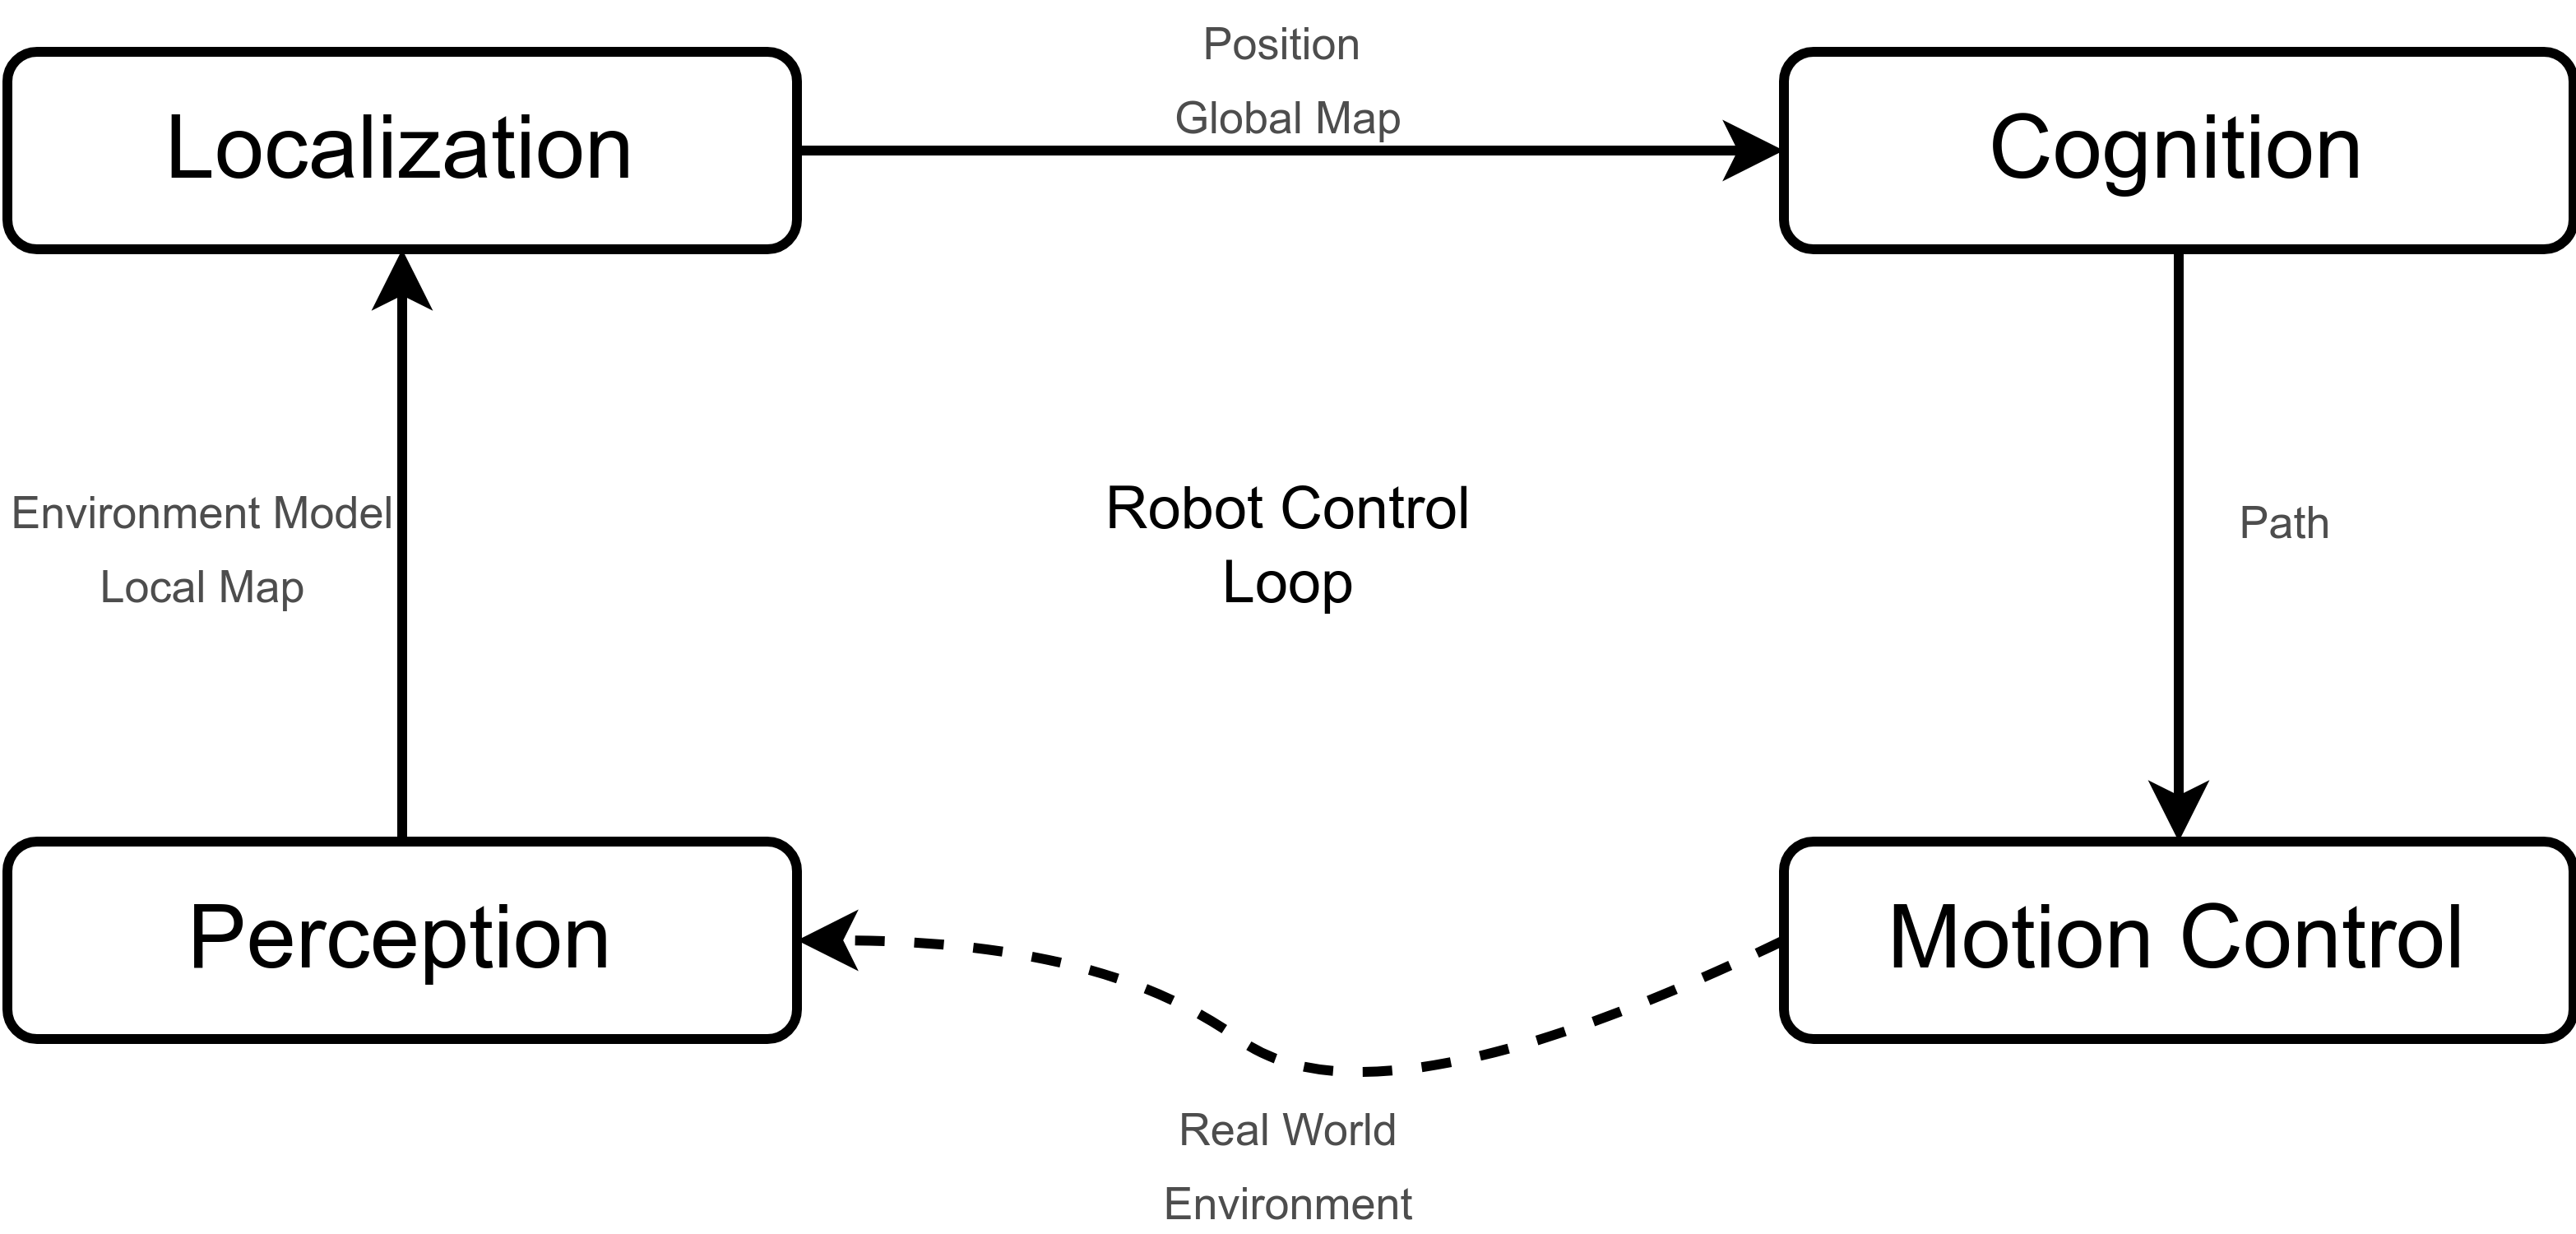
\includegraphics[width=4.6in, height=2.8in]{pics/navigation_overview.png}
    \caption[Overview of Navigation Problem]{Overview of Navigation Problem~\cite{ozkil2009navigation}}\label{nav_overview}
\end{figure}



\subsection{Localization and Mapping}
Localization is the process of determining the robot's position in the environment while mapping involves creating an internal
model of any unknown features in the environment~\cite{riisgaard2006slam}. Since both these processes are interdependent, a question arises whether it is
possible for a robot to perform self-localization when placed in an unknowned environment. This is widely referred to as
Simultaneous Localization and Mapping (SLAM) as Durrant Whyte depicts it in~\cite{durrant-whyte2006slam1} a ``holy grail'' for making the
dream of autonomous mobile robot come true. Researchers recently have proposed various algorithms to achieve SLAM in robot navigation and
as since some of these algorithms share similar steps in their design, there are many approaches to categorizing the techniques used in SLAM.\@
SLAM can be broadly categorized into two types based on the scale of localization:
\begin{enumerate}
    \item \textit{Global SLAM:} ability to determine the robot's position in an previously learned map, given no other information than
    that the robot is somewhere in the map.
    \item \textit{Local SLAM:} ability to track the robot's position over time, given that the robot's initial position is known (localized).
\end{enumerate}

\subsubsection{Dead Reckoning}
Dead reckoning is simple method that estimates the robot's current position based on its previously known position. The
position is determined using data from wheel encoders and inertial sensors like gyroscopes and accelerometers~\cite{borenstein1997mobile}.
While easy to implement and computationally efficient, dead reckoning can draw so many errors due to wheel slippage, uneven terrain, and
sensor noises or inaccuracies.This makes it unreliable for long-term navigation in unknown environments~\cite{PARK1998219}.
\subsubsection{Kalman Filters}
Kalman filters are recursive algorithms used to estimate the state of a dynamic system from a series of incomplete and noisy
measurements~\cite{thrun2005probabilistic}.\@ The foundation of KF is Bayes`s theorem, which combines prior knowledge of robot's position with new measurements to update
the estimate.
KF assumes that the system model is linear and the noise is Gaussian, which is represented by a normal distribution.
real-world scenarios. \\

\vspace{-0.2em}
\begin{itemize}
    \item \textbf{Prediction Step:}
    \begin{equation}
        \mu_{t|t-1} = A \mu_{t-1} + B u_{t-1}
    \end{equation}
    \vspace{-2.5em}
    \begin{equation}
        \Sigma_{t|t-1} = A \Sigma_{t-1} A^T + Q_t
    \end{equation}
    \vspace{-2.5em}
    
    where:
    \vspace{-0.3em}
    \begin{itemize}
        \item $\mu_{t|t-1}$ is the predicted state at time $t$.
        \item $\Sigma_{t|t-1}$ is the predicted covariance matrix.
        \item $A$ is the state transition model.
        \item $B$ is the control input model.
        \item $Q_t$ is the process noise covariance.
    \end{itemize}

    \item \textbf{Update Step:}
    \begin{equation}
        K_t = \Sigma_{t|t-1} C^T {\left(C \Sigma_{t|t-1} C^T + R_t\right)}^{-1}
    \end{equation}
    \vspace{-2.5em}
    \begin{equation}
        \mu_t = \mu_{t|t-1} + K_t (z_t - C \mu_{t|t-1})
    \end{equation}
    \vspace{-2.5em}
    \begin{equation}
        \Sigma_t = (I - K_t C) \Sigma_{t|t-1}
    \end{equation}
    \vspace{-1.5em}
    where:
    \vspace{0.5em}
    \begin{itemize}
        \item $K_t$ is the Kalman gain.
        \item $C$ is the observation model.
        \item $R_t$ is the measurement noise covariance.
        \item $z_t$ is the actual measurement update.
        \item $\delta_t \sim N(0, R_t)$ represents measurement noise.
    \end{itemize}
\end{itemize}

\begin{comment}
\textbf{Observation Model for KF:}
\begin{equation}
    z_t = C \mu_t + \delta_t
\end{equation}
where:
\begin{itemize}
    \item $\mu_t$ represents the true measurement without noise.
    \item $\delta_t$ is the noise, typically modeled as $N(0, R_t)$.
\end{itemize}
\end{comment}

\begin{algorithm}
    \caption{Kalman Filter Algorithm}\label{alg:kalman_filter}
    \begin{algorithmic}[1]
    \REQUIRE~Initial state estimate $\mu_0$, covariance $\Sigma_0$, sequence of observations $z_{1:t}$
    \ENSURE~Updated state estimate $\mu_{t}$
    \STATE\textbf{Function} \textsc{Predict} ($\mu_{t-1}, \Sigma_{t-1}, u_{t-1}$)
    \STATE\quad $\mu_{t|t-1} = A \mu_{t-1} + B u_{t-1}$
    \STATE\quad $\Sigma_{t|t-1} = A \Sigma_{t-1} A^T + Q_t$
    \STATE\quad $K_t = \Sigma_{t|t-1} C^T {\left(C \Sigma_{t|t-1} C^T + R_t\right)}^{-1}$
    \STATE\quad $\mu_{t} = \mu_{t|t-1} + K_t (z_t - C \mu_{t|t-1})$
    \STATE\quad $\Sigma_{t} = (I - K_t C) \Sigma_{t|t-1}$
    \STATE\quad \textbf{return} $\mu_{t}, \Sigma_{t}$
    \STATE\textbf{End Function}
    \end{algorithmic}
\end{algorithm}
    






\newpage
\subsubsection{Extended Kalman Filters (EKF)}
EKF uses the Extended Kalman Filter for probabilistic estimation of the robot's pose and landmark
positions~\cite{thrun2005probabilistic}. EKF can handle nonlinear systems by linearizing the observation and measurement models around the current estimate.
While KF assumes linearity, EKF addresses this limitation by approximating
the state transition and measurement models using the first-order Taylor expansion.

\begin{itemize}
    \item \textbf{Prediction Step:}
    \begin{equation}
        \mu_{t|t-1} = f(\mu_{t-1}, u_{t-1})
    \end{equation}
    \begin{equation}
        \Sigma_{t|t-1} = F_t \Sigma_{t-1} F_t^T + Q_t
    \end{equation}
    where:
    \begin{itemize}
        \item $f(\cdot)$ is the nonlinear state transition function.
        \item $F_t$ is the Jacobian matrix of the state transition function with respect to the state.
    \end{itemize}

    \item \textbf{Update Step:}
    \begin{equation}
        K_t = \Sigma_{t|t-1} H_t^T {(H_t \Sigma_{t|t-1} H_t^T + R_t)}^{-1}
    \end{equation}
    \begin{equation}
        \mu_t = \mu_{t|t-1} + K_t (z_t - h(\mu_{t|t-1}))
    \end{equation}
    \begin{equation}
        \Sigma_t = (I - K_t H_t) \Sigma_{t|t-1}
    \end{equation}
    where:
    \begin{itemize}
        \item $h(\cdot)$ is the nonlinear measurement function.
        \item $H_t$ is the Jacobian matrix of the measurement function.
    \end{itemize}
\end{itemize}


\begin{algorithm}
    \caption{Extended Kalman Filter Algorithm}\label{alg:ekf}
    \begin{algorithmic}[1]
    \REQUIRE~Initial state estimate $\mu_0$, covariance $\Sigma_0$, sequence of observations $z_{1:t}$
    \ENSURE~Updated state estimate $\mu_{t}$
    \STATE\textbf{Function} \textsc{Predict} ($\mu_{t-1}, \Sigma_{t-1}, u_{t-1}$)
    \STATE\quad $\mu_{t|t-1} = f(\mu_{t-1}, u_{t-1})$
    \STATE\quad $\Sigma_{t|t-1} = F_t \Sigma_{t-1} F_t^T + Q_t$
    \STATE\quad $K_t = \Sigma_{t|t-1} H_t^T {(H_t \Sigma_{t|t-1} H_t^T + R_t)}^{-1}$
    \STATE\quad $\mu_{t} = \mu_{t|t-1} + K_t (z_t - h(\mu_{t|t-1}))$
    \STATE\quad $\Sigma_{t} = (I - K_t H_t) \Sigma_{t|t-1}$
    \STATE\quad \textbf{return} $\mu_{t}, \Sigma_{t}$
    \STATE\textbf{End Function}
    \end{algorithmic}
\end{algorithm}

    
\newpage
\subsubsection{Particle Filters (Monte Carlo Localization (MCL))}
Particle filters represent the robot's belief of its position using a set of weighted samples (particles)~\cite{thrun2005probabilistic}.
Each particle represents a possible pose, and the weights are updated based on sensor measurements (observation model) and robot's
movement (motion model). With contrast to KF and EKF, particle filters can handle nonlinear and non-Gaussian systems, thus they have
the ability to globally (re-)~localize the robot in the case of localization failures. 
\vspace{-0.3em}
\vspace{-0.5em}
\begin{itemize}
    \item \textbf{Prediction Step:}
    \begin{equation}
        x_t^{[i]} = f(x_{t-1}^{[i]}, u_t) + \epsilon_t
    \end{equation}
    \vspace{-0.5em}
    where:
    \begin{itemize}
        \item $x_t^{[i]}$ is the state of particle $i$ at time $t$.
        \item $u_t$ is the control input.
        \item $\epsilon_t$ is the noise term.
    \end{itemize}
    \vspace{-0.7em}
    \item \textbf{Update Step:}
    \begin{equation}
        w_t^{[i]} = p(z_t | x_t^{[i]})
    \end{equation}
    \vspace{-0.5em}
    where:
    \begin{itemize}
        \item $w_t^{[i]}$ is the weight of particle $i$.
        \item $p(z_t | x_t^{[i]})$ is the likelihood of the measurement $z_t$ given the particle state.
    \end{itemize}

    \item \textbf{Resampling Step:}
    \begin{equation}
        N_{\text{eff}} = \frac{1}{\sum_{i=1}^{N} {(w_t^{[i]})}^2}
    \end{equation}
    Resample particles if $N_{\text{eff}}$ is below a threshold to avoid particle depletion.
\end{itemize}

\begin{algorithm}
    \caption{Monte Carlo Localization Algorithm}\label{alg:mcl}
    \begin{algorithmic}[1]
    \REQUIRE~Initial set of particles $\{x_0^{[i]}{\}}_{i=1}^{N}$, sequence of observations $z_{1:t}$
    \ENSURE~Updated particles $\{{x_t}^{[i]}, w_t^{[i]}{\}}_{i=1}^{N}$
    \FOR{each particle $i$}
        \STATE~Predict new state $x_t^{[i]} = f(x_{t-1}^{[i]}, u_t) + \epsilon_t$
        \STATE~Update weight $w_t^{[i]} = p(z_t | x_t^{[i]})$        
    \ENDFOR\STATE~Resample particles if necessary based on $N_{\text{eff}}$
    \STATE\textbf{return} $\{{x_t}^{[i]}, w_t^{[i]}{\}}_{i=1}^{N}$
    \end{algorithmic}
\end{algorithm}



\subsubsection{Adaptive Monte Carlo Localization (AMCL)}
AMCL extends MCL by adapting the number of particles dynamically based on the uncertainty in the robot’s pose.
This adaptive approach helps in balancing the computational cost and the localization accuracy. A more detailed
explanation of this algorithm will be explained in the methodologies section.

\begin{algorithm}
    \caption{Adaptive Monte Carlo Localization (AMCL) Algorithm}\label{alg:amcl}
    \begin{algorithmic}[1]
    \REQUIRE~Initial set of particles $\{x_0^{[i]}{\}}_{i=1}^{N}$, sequence of observations $z_{1:t}$
    \ENSURE~Updated particles $\{{x_t}^{[i]}, w_t^{[i]}{\}}_{i=1}^{N}$
    \FOR{each particle $i$}
        \STATE~Predict new state $x_t^{[i]} = f(x_{t-1}^{[i]}, u_t) + \epsilon_t$
        \STATE~Update weight $w_t^{[i]} = p(z_t | x_t^{[i]})$
    \ENDFOR\STATE~Calculate $N_{\text{eff}} = \frac{1}{\sum_{i=1}^{N} {(w_t^{[i]})}^2}$
    \IF{$N_{\text{eff}} < N_{\text{threshold}}$}
        \STATE~Resample particles
        \STATE~Adjust particle count dynamically based on pose uncertainty    
    \ENDIF\STATE~\textbf{return} $\{{x_t}^{[i]}, w_t^{[i]}{\}}_{i=1}^{N}$
    \end{algorithmic}
\end{algorithm}


\subsubsection{Hector SLAM}
Hector SLAM represents a significant advancement in 2D SLAM algorithms, particularly notable for
its ability to operate without odometry information, relying solely on high-resolution LiDAR data~\cite{nagla2020hector}. 
This characteristic makes it especially suitable for medical autonomous navigation systems where wheel odometry might be
unreliable due to smooth hospital floors or frequent starts and stops.

\noindent The algorithm employs a scan-matching approach based on the Gauss-Newton optimization method, which can be expressed mathematically as:

\begin{equation}
x_t = \arg \min \sum_{i=1}^{n} {[1 - M{(S_i{(x_t)})}]}^2
\end{equation}

\noindent where $x_t$ represents the optimal pose of the LiDAR, and $M(S_i(x_t))$ denotes the grid map value at coordinate $S_i(x_t)$.
However, Hector SLAM's performance can be limited in environments with few geometric features or in situations requiring long-term consistency over large areas. For medical applications, this suggests its optimal use would be in well-structured hospital environments where regular updates to the map can be performed.


\newpage


\subsubsection{Google Cartographer}
Google Cartographer is a 2D and 3D SLAM algorithm that uses both LiDAR and IMU 
data. Originally developed by W.Hess~\cite{hess2021real} for Google's street mapping, it has
been adapted for indoor robotics applications. For the 2D case, it features a loop-closure detection to 
create submaps known as ``ground-truth''. Optimization is done on the generated submaps to have a trajectory
relation between two trajectory nodes. A LiDAR communicates with the ROS through a topic after doing the 
environment scan~\cite{ramadhan2021design}. The data is then processed by the cartographer node, which is responsible for the 
processing of the data in real-time and outputting the trajectory and map to a visualization software like Rviz. A 
depiction is shown in the figures~\ref{cart1} and~\ref{cart2} below.


\vspace{3em}

\begin{figure}[H]
    \centering
    \begin{minipage}{0.41\textwidth}
        \centering
        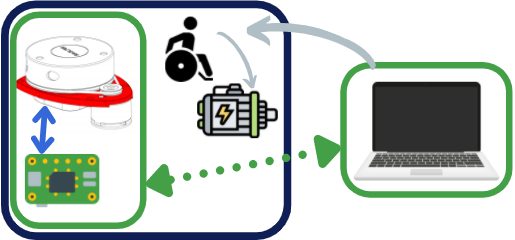
\includegraphics[width=\linewidth]{pics/cart1.png}
        \caption[System representation]{System representation~\cite{ramadhan2021design}}\label{cart1}
    \end{minipage}\hfill
    \begin{minipage}{0.48\textwidth}
        \centering
        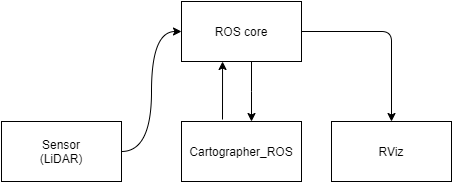
\includegraphics[width=\linewidth]{pics/cart2.png}
        \caption[System data workflow]{System data workflow~\cite{ramadhan2021design}}\label{cart2}
    \end{minipage}\hfill
\end{figure}

\vspace{0.25cm}

\subsubsection{Grid-based FastSLAM (Gmapping)}
GMapping is a highly efficient Rao-Blackwellized particle filter (RBPF) that separates the estimation of the
robot's trajectory hypothesis and the map~\cite{grisetti2007improved}. GMapping effectively builds accurate grid maps
in real-time and is well-suited for indoor environments. The key innovation of Grid-based FastSLAM lies
in its improved proposal distribution that considers both odometry data and the most recent sensor
observations when generating new particles. This approach significantly reduces the number of
particles required for accurate mapping compared to traditional methods that rely solely on odometry
motion models~\cite{1570477}. For medical environments where precise navigation is
crucial, this efficiency is particularly valuable as it enables real-time performance with limited
computational resources. However, the algorithm's performance can be affected in environments 
with limited features or highly symmetric structures, which may require additional sensing modalities or environmental modifications to ensure reliable operation in medical settings.


\newpage

\subsection{Path Planning}
Path planning enables the robot to navigate from a starting
location to a desired goal while avoiding obstacles. Effective path planning algorithms compute feasible and
optimal paths, taking into account the robot's kinematics, dynamics, and the environment's constraints. This section
reviews several key path planning algorithms: Dijkstra's Algorithm, A* Algorithm, Rapidly-exploring Random Trees (RRT),
and the Dynamic Window Approach (DWA).


\subsubsection{Dijkstra's Algorithm}
Dijkstra's algorithm, developed by E. Dijkstra in 1959, represents an approach to solving the single-source shortest path problem in weighted graphs. The algorithm determines the minimum cost path from a source vertex to all other vertices in a graph with non-negative edge weights. For a directed weighted graph \(G = (V,E)\), where \(V\) represents the set of vertices and \(E\) the set of edges, Dijkstra's algorithm maintains a set \(S\) of vertices whose final shortest-path weights from the source have been determined. The algorithm operates by iteratively selecting the vertex \(u \in V - S\) with the 
minimum shortest-path estimate, adding \(u\) to \(S\), and relaxing all edges leaving \(u\). The core evaluation function can be expressed as:

\begin{equation}
    d(v) = \min \{d(u) + w(u,v)\}
\end{equation}

\noindent where \(d(v)\) represents the shortest distance to vertex \(v\), \(d(u)\) is the distance to the current vertex \(u\), and \(w(u,v)\) is the weight of the edge connecting vertices \(u\) and \(v\).



\noindent While Dijkstra's algorithm guarantees finding the optimal path in static 
environments, experimental analysis has shown that it explores significantly more nodes
than informed search methods like A*. As demonstrated in the comparative study
by~\cite{alija2015analysis}, Dijkstra's algorithm exhibits an average search time
approximately 466ms slower than A* in grid-based environments, despite both algorithms
finding paths of identical length.

\newpage

\subsubsection{A* Algorithm}
The A* algorithm represents one of the most efficient heuristic search methods for finding optimal paths in static environments~\cite{gul2019comprehensive}. Its effectiveness stems from combining Dijkstra's algorithm's thoroughness with the added benefit of heuristic estimation. The algorithm employs an evaluation function \(F(n)\) that consists of two components:

\begin{equation}
    F(n) = G(n) + H(n)
\end{equation}

\noindent where \(G(n)\) represents the actual cost from the start node to the current node \(n\), and \(H(n)\) is the heuristic estimated cost from node \(n\) to the goal. The heuristic component \(H(n)\) can be calculated using various distance metrics, as illustrated in Figure~\ref{fig:astar_distances}.

\begin{figure}[H]
    \centering
    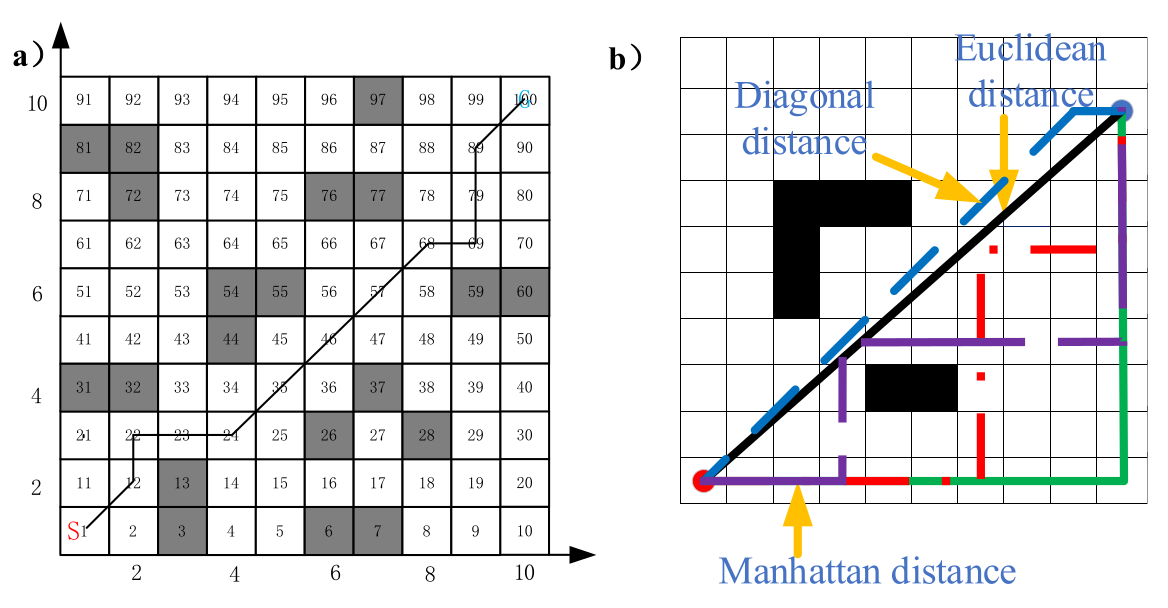
\includegraphics[width=5.5in]{pics/astar_distances.png}
    \caption[Schematic diagram of grid method and paths generated by different distance functions]{(\textbf{a}) Schematic of A* grid (\textbf{b}) Paths from different distance functions~\cite{xiang2022combined}}\label{fig:astar_distances}
\end{figure}

\noindent Recent improvements to the traditional A* algorithm have addressed several key limitations
through three primary enhancements. First, the incorporation of obstacle information into the 
evaluation function improves convergence speed and path quality, modifying the function to:

\begin{equation}
    F(n) = G(n) + H(n) + o(n)
\end{equation}

\noindent where \(o(n)\) represents the obstacle information weight. Second, adaptive directional search has been implemented to reduce unnecessary node expansions by focusing on promising directions based on the target position. Third, path smoothing optimization removes redundant waypoints while maintaining path safety, resulting in approximately 5\% reduction in total path length~\cite{xiang2022combined}.

\newpage

\subsubsection{Rapidly-exploring Random Trees (RRT)}
Rapidly-exploring Random Trees (RRT) is a sampling-based path planning algorithm designed for efficiently searching high-dimensional spaces~\cite{ganesan2024hybrid}. It incrementally builds a space-filling tree by randomly sampling points in the space and connecting them to the nearest node in the tree. The algorithm begins with the initialization step, starting with the initial position of the robot as the root node of the tree. In the sampling loop, a point \(q_{\text{rand}}\) is randomly sampled in the space. The nearest node \(q_{\text{near}}\) in the tree to \(q_{\text{rand}}\) is found, and the algorithm moves from \(q_{\text{near}}\) towards \(q_{\text{rand}}\) by a predetermined step size to get \(q_{\text{new}}\). If the path from \(q_{\text{near}}\) to \(q_{\text{new}}\) is collision-free, \(q_{\text{new}}\) is added to the tree. The process terminates when \(q_{\text{new}}\) is close enough to the goal, allowing for the reconstruction of the path.

\vspace{-0.02cm}

\begin{algorithm}[H]
    \caption{RRT* Framework}\label{alg:rrt}
    \begin{algorithmic}[1]
    \STATE $T \leftarrow (V, E)$
    \FOR{all values of i from 0 to N}
        \STATE $q_{\text{rand}} \leftarrow \text{uniformsample}(i)$
        \STATE $q_{\text{nearest}} \leftarrow \text{nearestneighbors}(T,q_{\text{rand}})$
        \STATE $(\sigma, q_{\text{new}}) \leftarrow \text{steer}(q_{\text{nearest}},q_{\text{rand}})$
        \IF{$\text{obstaclefree}(\sigma)$}
            \STATE $Q_{\text{near}} \leftarrow \text{nearnode}(q_{\text{new}},T)$
            \STATE $(q_{\text{parent}},\sigma_{\text{parent}}) \leftarrow \text{parentupdate}(Q_{\text{near}},q_{\text{nearest}},q_{\text{new}},\sigma)$
            \STATE $T \leftarrow \text{add}(T,q_{\text{parent}},q_{\text{new}},\sigma_{\text{parent}})$
            \STATE $T \leftarrow \text{Rewire}(q_{\text{new}},T,Q_{\text{near}})$
        \ENDIF
    \ENDFOR
    \RETURN $T$
    \end{algorithmic}
\end{algorithm}

\noindent The RRT* algorithm represents a significant advancement in sampling-based path planning, particularly suited for high-dimensional spaces~\cite{karaman2011sampling}. It employs an iterative tree construction process that begins with the robot's initial configuration. The algorithm generates uniform random samples ($q_{\text{rand}}$) across the configuration space and extends the tree by connecting these samples to the nearest existing nodes ($q_{\text{nearest}}$). A key feature of RRT* is its rewiring mechanism, which continuously optimizes the tree structure by checking for potentially shorter paths through new connections.

\noindent Recent improvements to RRT* have addressed its limitations through various sampling strategies. For instance, hybrid sampling approaches combine uniform and non-uniform sampling methods to balance exploration and exploitation~\cite{ganesan2024hybrid}. This hybrid approach has demonstrated superior performance in terms of convergence rate, success rate, and computational efficiency compared to traditional RRT* implementations, achieving up to 76.14\% faster average convergence rates while reducing node exploration by approximately 48.53\%.

\vspace{-0.08cm}

\begin{figure}[H]
    \centering
    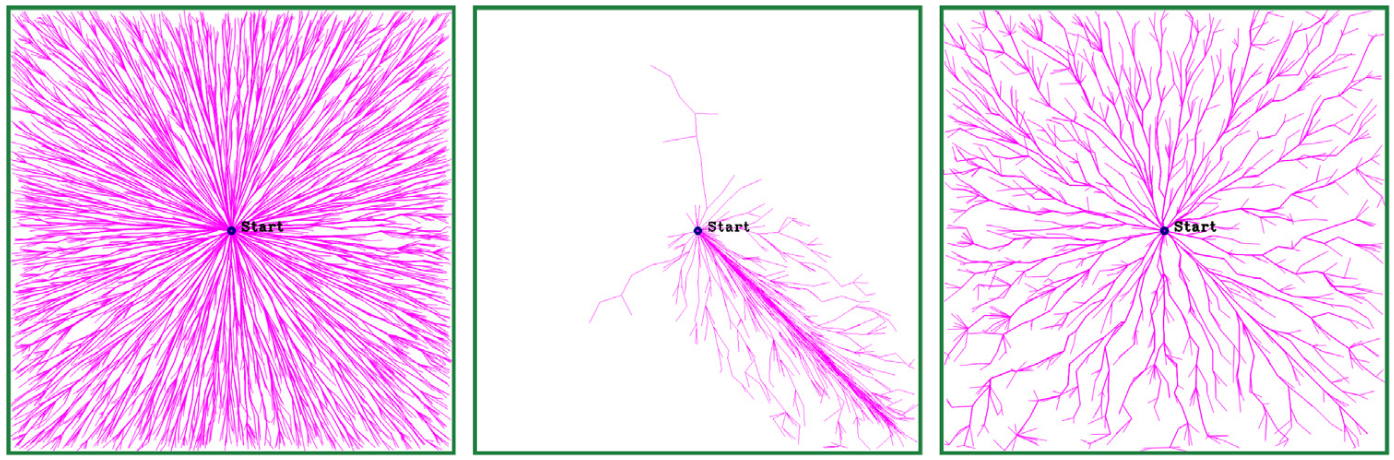
\includegraphics[width=5.2in]{pics/rrt.png}
    \caption[Tree exploration of (\textbf{a}) RRT* and (\textbf{b}) RRT* Connect]{Tree exploration of (\textbf{a}) RRT* and (\textbf{b}) Informed RRT* (\textbf{c}) RRT*-N~\cite{ganesan2024hybrid}}\label{fig:rrt}
\end{figure}

\noindent RRT is efficient in handling high-dimensional and complex spaces and exhibits probabilistic completeness, meaning it will find a solution if one exists given enough time. However, the paths generated may be non-optimal and require smoothing, and the random nature of the algorithm can lead to inconsistent performance. RRT is particularly useful in robotic manipulators and autonomous vehicles where the configuration space is high-dimensional.

\vspace{-0.02cm}

\begin{figure}[H]
    \centering
    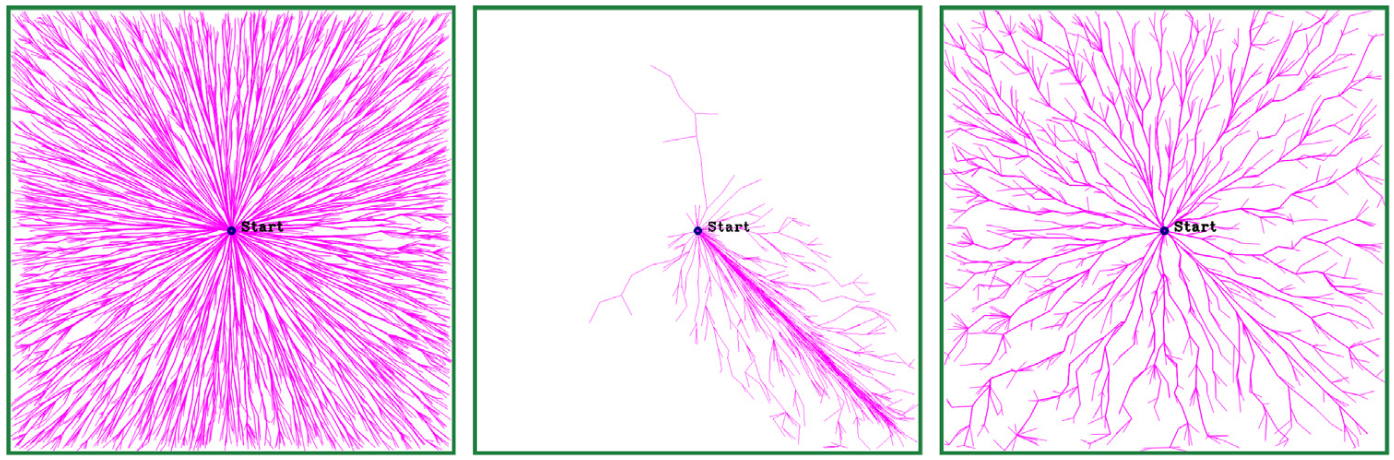
\includegraphics[width=5.2in]{pics/rrt.png}
    \caption[Tree exploration of (\textbf{a}) RRT* and (\textbf{b}) RRT* Connect]{Tree exploration of (\textbf{a}) RRT* and (\textbf{b}) Informed RRT* (\textbf{c}) RRT*-N~\cite{ganesan2024hybrid}}\label{fig:rrt}
\end{figure}


\newpage

\subsubsection{Dynamic Window Approach (DWA)}
The Dynamic Window Approach is a local trajectory planning method that considers
the robot's dynamics to generate feasible and safe motion commands. The algorithm operates by defining
the set of possible velocities considering the robot's current velocity, acceleration limits, and kinematic constraints. A dynamic window limits the velocity space to velocities achievable within a short time frame. For each velocity in the dynamic window, the algorithm simulates the trajectory and evaluates it based on heading (alignment towards the goal), clearance (distance from obstacles), and velocity (preference for higher speeds). The velocity that 
maximizes the objective function, combining the above criteria, is selected. DWA generates motion commands
that are dynamically feasible and allows for real-time obstacle avoidance. However, as a local planner, it may not find a path around large obstacles, suffering from the local minima problem. It requires a good balance between the evaluation criteria. DWA is widely used for real-time navigation in dynamic environments where obstacles may move unpredictably.






\subsection{Robot Operating System 2 (ROS2)}
Since robotic systems involve a combination of many fields in engineering, the task at hand can be complex
and challenging when it comes to integration.
The Robot Operating System 2 (ROS2), formally ROS,  although not an operating system in a traditional sense, is a an open-source framework that provides tools,
libraries, and conventions designed to simplify the task of creating robots.   

\vspace{1.0em}
\begin{figure}[H]
    \centering
    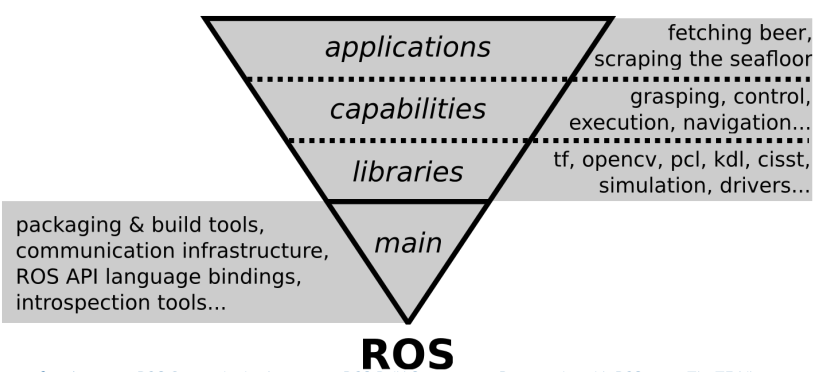
\includegraphics[width=4.8in ]{pics/ree.png}
    \caption[Levels of development with ROS]{Levels of development with ROS~\cite{mosenlechner2012ros}}\label{lt_4}
\end{figure}


\newpage

\subsection{Navigation frameworks in ROS2}
Since robotic applications have different specific requirements, such as indoor or outdoor applications, 3D navigation
with the example of a drone to 2D navigation with the example of a SCARA robot or different optimizations, there are
several frameworks used for robot navigation. Some of the frameworks which are commonly integrated within ROS2 are
explored in this section. 

\subsubsection{Navigation 2 Stacks (Nav2)}
Navigation2~\cite{thomas2014nextgenros}\cite{macenski2020marathon2} is a navigation framework specifically designed for ROS2~\cite{thomas2014nextgenros}, which was built as an improvement on
the previous ROS Navigation~\cite{quigley2009ros} for ROS~\cite{mardereppstein2010office}. It provides a flexible and modular framework for autonomous
navigation~\cite{macenski2020marathon2}. It features behavior trees~\cite{abiyev2016robot} for task execution, a plugin-based architecture
for custom planners and controllers, improved performance leveraging ROS2`s real-time capabilities, and 
costmaps for planning and obstacle avoidance. Nav2 supports various navigation algorithms, making it easier to implement 
techniques like SLAM (Simultaneous Localization and Mapping) and AMCL (Adaptive Monte Carlo Localization). Nav2 
integrates A* and Dijkstra's Algorithm in the global planner to compute optimal paths on a costmap grid, allowing
for the customization of planners as per requirements. For example,  the Dynamic Window Approach (DWA) can
be used in the local planner to compute velocity commands that are safe and feasible, considering the robot's
dynamic constraints and real-time sensor data. Nav2’s flexibility, modularity, and real-time capabilities make
it suitable for a wide range of robots.


\vspace{0.7em}
\begin{figure}[H]
    \centering
    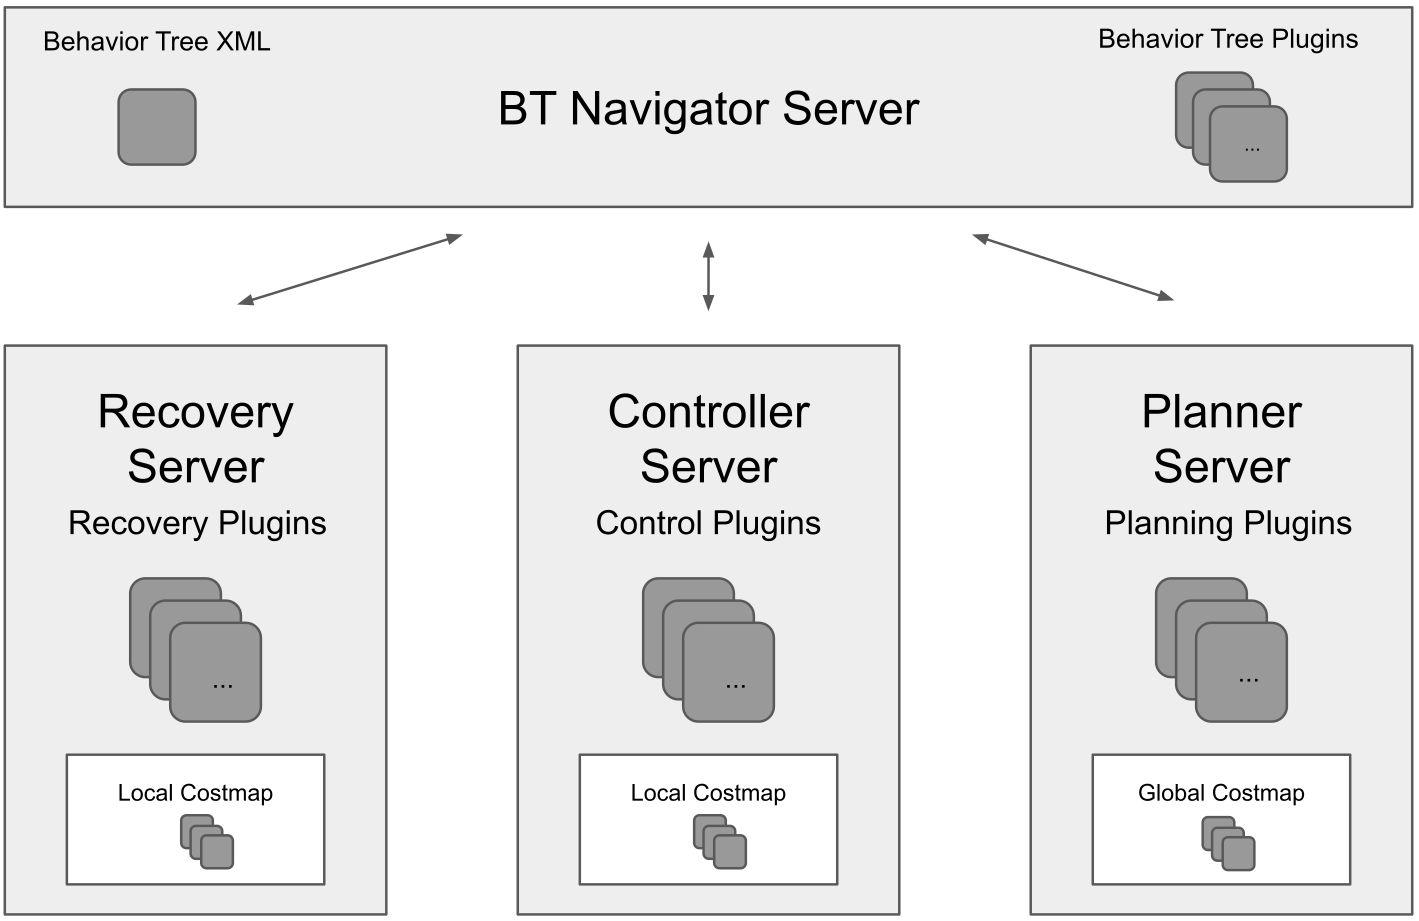
\includegraphics[width=4.5in ]{pics/nav2.png}
    \caption[Overview of Navigation2 design]{Overviewof Navigation2 design~\cite{macenski2020marathon2}}\label{nav2}
\end{figure}


\subsubsection{ARC Nav Stack}
Since most of the existing navigation stacks implemented on ROS and its successor ROS2 are primarily designed for 2D navigation
environments, the approach simplifies computations but it is only suitable for wheeled robots navigating on flat surfaces. There
are serious limitations when dealing with robots that operate in three-dimensional (3D) environments, such as aerial drones or legged
robots traversing uneven terrain. The ARC Nav Stack was introduced~\cite{vishwas2021arc} to overcome this limitation. ARC Nav
utilizes a volumetric representation of the robot's workspace, thus enabling full 3D motion planning and control. ARC Nav uses the OctoMap~\cite{hornung2013octomap}
library for mapping, that represents 3D space using an octree data structure. OctoMap allows for the probabilistic
representation of occupancy, handling sensor noise and uncertainties effectively. The use of an octree structure enables
the compression of the map by recursively combining neighboring voxels with similar information, reducing memory
consumption while maintaining essential details of the environment. ARC Nav is crucial for safe navigation and exploration tasks~\cite{vishwas2021arc}.


\vspace{0.7em}
\begin{figure}[H]
    \centering
    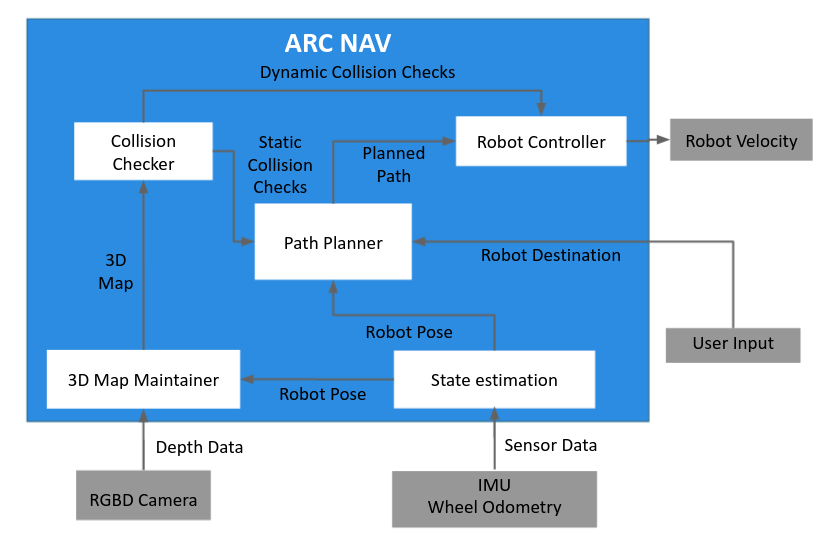
\includegraphics[width=4.0in ]{pics/arc_nav.png}
    \caption[Overview of the ARC Nav Stack Architecture]{Overview of the ARC Nav Stack Architecture~\cite{vishwas2021arc}}\label{arc4}
\end{figure}




\noindent In terms of motion planning, ARC Nav introduces a novel sampling-based algorithm called 2BIT*, which extends the Batch Informed
Trees (BIT*) algorithm~\cite{gammell2015bit} by incorporating a bidirectional search approach. Traditional BIT* combines features
from algorithms like Fast Marching Tree (FMT*) and Informed RRT*, focusing on efficiency and optimality in path planning. The 2BIT* algorithm
enhances BIT* by growing two trees simultaneously: one rooted at the start position and the other at the goal position. These trees expand towards each other, aiming to find a connection that results in a feasible path.

\noindent A key innovation in 2BIT* is the introduction of strategy switching during the connection attempts between the two trees.
Two primary strategies are employed: connecting the most recently added node of one tree to the nearest node in the other
tree, and connecting it to a randomly chosen node. By allocating probabilities to each strategy and switching between them
based on certain conditions, the algorithm adapts to the planning scenario, reducing the time taken to find an initial
path and improving convergence towards the shortest possible path. This adaptive approach addresses the 
limitations observed in algorithms like RRT-Connect~\cite{Kuffner2000RRTconnectAE}, which, while efficient in finding initial
paths, do not guarantee asymptotic optimality and lack strategy variability. 
The architecture of ARC Nav is modular, similar to Nav2, allowing for easy customization of components like state estimation,
mapping, planning, and control. 



\subsubsection{RTAB-Map}

A 2D lidar sensor mounted at a fixed height may fail to detect overhanging obstacles like tables and chairs
or low-lying objects such as trash cans, leading to incomplete maps and potential navigation failures.To address these challenges~\cite{labbe2018rtabmap} explored the use of RTAB-Map (Real-Time Appearance-Based Mapping), a graph-based SLAM approach that integrates
data from multiple sensors to generate comprehensive 3D maps. By fusing information from an RGB-D camera, a 2D lidar, an IMU, and wheel odometry, the robot can construct a more accurate representation of its environment, enhancing navigation and obstacle avoidance capabilities.



\vspace{0.7em}
\begin{figure}[H]
    \centering
    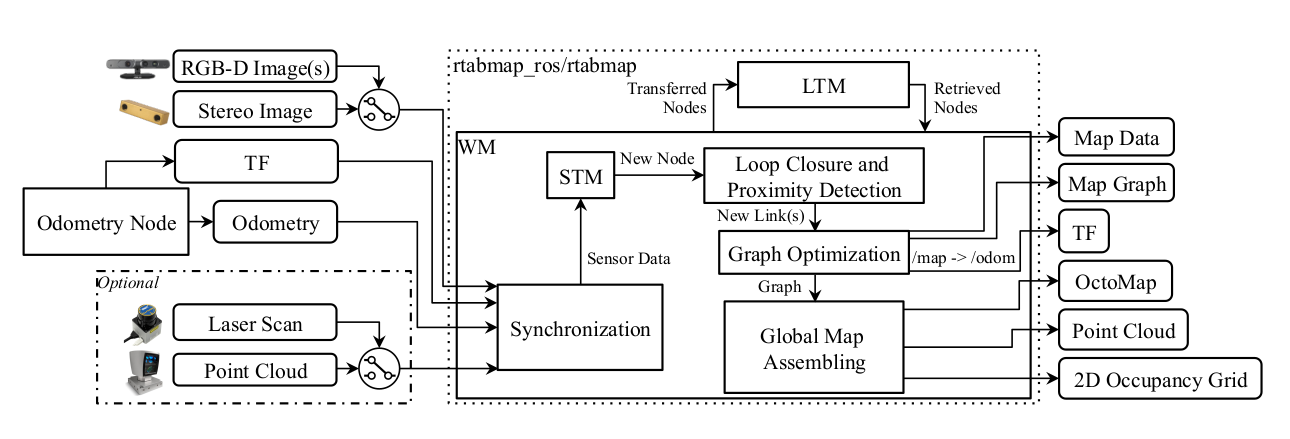
\includegraphics[width=6.3in, height=3.2in]{pics/rtab1.png}
    \caption[Schematic flowchart of RTAB-Map]{Schematic flowchart of RTAB-Map~\cite{labbe2018rtabmap}}\label{rtab_flow}
\end{figure}



\subsubsection{Micro-ROS}
Mobile robots are becoming more complex and integrating microcontrollers into their architectures is 
essential for modularity and efficient
resource management. Micro-ROS is designed for microcontrollers and embedded systems thus it can integrate 
them with ROS2. In~\cite{nguyen2022microros}, MicroROS
was evaluated on the quality of service (QoS) and communication capabilities. Micro-ROS is optimized for 
low memory usage and efficient
processing, it utilizes a lightweight communication protocol called DDS for Extremely Resource Constrained 
Environments (DDS-XRCE)~\cite{nguyen2022microros},
which allows micro-ROS clients on microcontrollers to communicate efficiently with teh micro-ROS agent. 
The micro-ROS agent, running on a more powerful processor, acts as a bridge between the micro-ROS client 
and the ROS 2 network, translating communication between DDS-XRCE and the standard DDS protocol used by 
ROS 2 nodes.


\vspace{0.7em}
\begin{figure}[H]
    \centering
    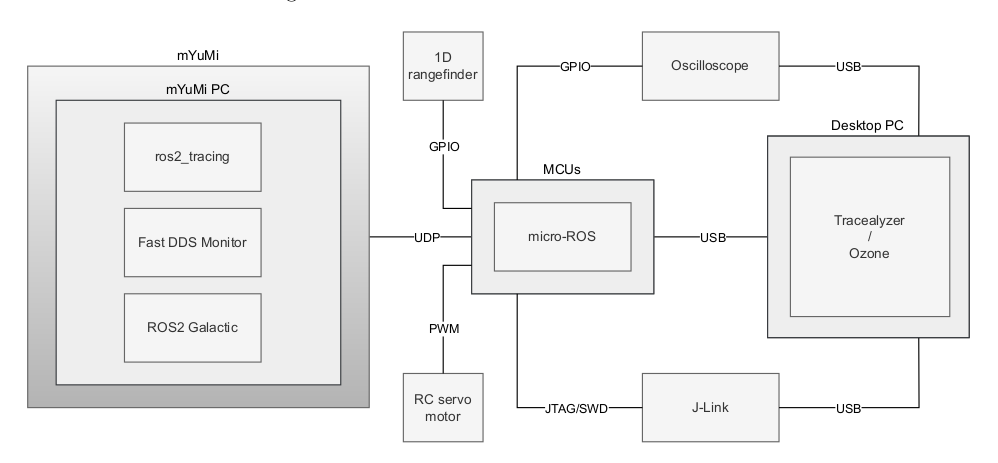
\includegraphics[width=6.4in ]{pics/microROS.png}
    \caption[Micro-ROS connecting mYuMi robot to MCUs]{Micro-ROS connecting mYuMi robot to MCUs~\cite{nguyen2022microros}}\label{microros}
\end{figure}



\subsubsection{Autoware-Based Navigation}
Autoware is an open-source software stack specifically designed for autonomous driving applications, providing an extensive
range of functionalities required for self-driving vehicles, including perception, localization, planning, and control. 
Built on top of ROS 2, Autoware integrates data from various sensors such as lidars, cameras, GPS, and IMUs to perceive the 
environment and accurately localize the vehicle within it. The framework employs advanced algorithms for object detection, 
lane recognition, and obstacle avoidance, enabling vehicles to navigate complex urban environments.

\noindent Autoware`s modular and adaptable design allows developers to tailor the system to specific vehicles and 
operational
requirements. An integral part of this ecosystem is Autoware
Perf, a tracing and performance analysis framework developed to evaluate and optimize the performance of ROS 2 applications
within Autoware. AutowarePerf extends existing tracing tools, such as ROS 2 Tracing and LTTng, to measure execution times 
of nodes and inter-node communication latencies. This framework enables developers to gain insights into the system's 
end-to-end latency, identify bottlenecks, and optimize performance to meet real-time constraints essential for autonomous vehicles.
By providing detailed performance metrics and visualization tools, Autoware Perf facilitates the development of 
high-performance, reliable autonomous driving systems. It addresses challenges such as selective measurement of specific nodes, 
insertion of trace points for communication latency measurement, and overall latency calculation across the system. 
Through these capabilities, Autoware and its associated tools contribute significantly to the advancement of autonomous vehicle 
technologies, emphasizing safety, efficiency, and scalability.\\

\vspace{0.005in}

\subsubsection{Comparison of ROS2 Navigation Frameworks}

\begin{table}[h]
    \centering
    \renewcommand{\arraystretch}{2.0}
    \setlength{\tabcolsep}{4.4pt}
    \footnotesize
    \begin{tabular}{|p{2.4cm}|p{2.2cm}|p{2.95cm}|p{1.9cm}|p{4.7cm}|}
      \hline
      \rowcolor[gray]{0.8} 
      \textbf{Framework} & \textbf{\makecell[{{l}}]{Dimensions\\Supported}} & \textbf{Primary Sensors} & \textbf{Complexity} & \textbf{Ideal Applications} \\
      \hline
      Nav2 & 2D & LIDAR, 2D Sensors, Odometry & Medium & Indoor ground mobile robots on flat surfaces\\
      \hline
      ARC Nav & 3D & Depth Cameras, 3D LIDAR & High & Drones, underwater vehicles, multi-level navigation\\
      \hline
      RTAB-Map & 3D & RGB-D and Stereo Cameras, LIDAR & High & 3D mapping (High-precision), exploration \\
      \hline
      Cartographer & 2D and 3D & Lidar, IMU & High & Real-time SLAM, indoor (High-precision) mapping \\
      \hline
      Hector SLAM & 2D & LIDAR & Medium & Fast mapping without odometry, indoor navigation \\
      \hline
      Gmapping & 2D & LIDAR, Odometry & Medium & Indoor SLAM with wheel odometry \\
      \hline
      Micro-ROS & 2D (primarily) & \makecell[{{l}}]{\raisebox{-1.5pt}{Various embedded}\\sensors} & Low & Resource-constrained devices \\
      \hline
      Autoware-Based Navigation & 3D & LIDAR, GPS, IMU, Camera & High & Autonomous driving \\
      \hline
    \end{tabular}
    \caption{Comparison of ROS2 Navigation Frameworks}\label{tab:comparison_ros2_navigation_frameworkss}
\end{table}


\newpage
\subsection{Related Works}
\subsubsection{Navigation with Gmapping and AMCL}
\noindent In~\cite{kok2020intelligent}, a medical robot which uses ROS was implemented for assistance and conveyance of incoming patients in a hospital. The shortest distance algorithm approach
was was utilized, while the Grid-based mapping (Gmapping) is employed to map the environment. Gazebo and Rviz are visualization tools which were
also used in this research. For patient-staff communication, a voice recognition system that integrates with ROS firmware mapping algorithm is done. On the user interface design, the user
can communicate with the robot and even see the locations where robot can go~\cite{kok2020intelligent}. The Policlinic in visualized in
RviZ tool as can be seen in the \figref{lt_1} below. The robot uses the Adaptive Monte Carlo Localization (AMCL)~\cite{chung2022improved} algorithm for localization and that combined
with the mapping algorithm achieves what is known as Simultaneous Localization and Mapping (SLAM). 


\begin{figure}[H]
    \centering
    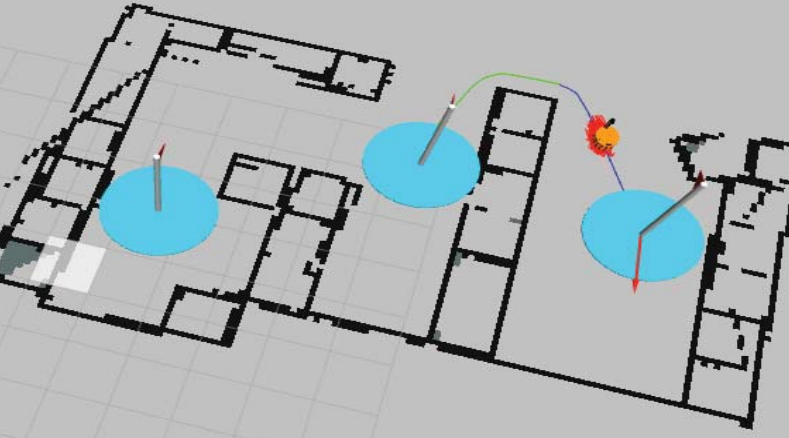
\includegraphics[width=3.2in]{pics/lt_1.png}
    \caption[Localization of the Policlinic in Rviz simulation tool]{Localization of the Policlinic in Rviz simulation tool~\cite{kok2020intelligent}}\label{lt_1}
\end{figure}

\begin{figure}[H]
    \centering
    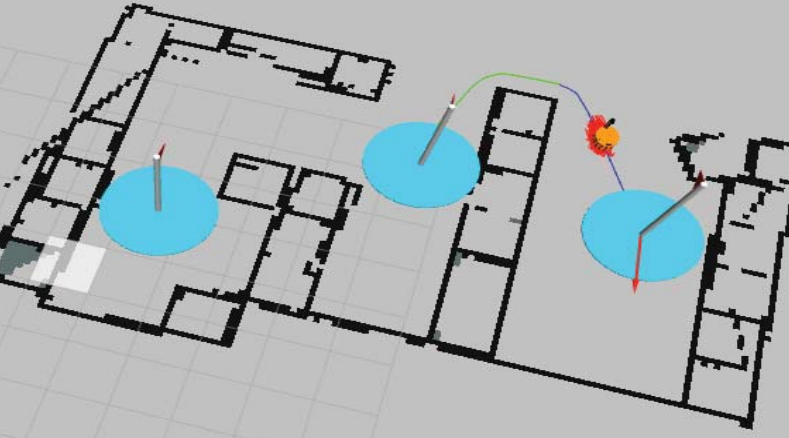
\includegraphics[width=3.2in]{pics/lt_1.png}
    \caption[Localization of the Policlinic in Rviz simulation tool]{Localization of the Policlinic in Rviz simulation tool~\cite{kok2020intelligent}}\label{lt_1}
\end{figure}

\subsubsection{Navigation with RGB-D}
\noindent Another relevant study focuses on positioning and navigation of a medical robot by the use of
RGB-D cameras. These cameras provide color and depth information of an image hence are more accurate and 
very suitable for environmental mapping. This approach supercedes the traditional SLAM algorithms by 
enhancing feature point extraction and mismatch elimination using Random Sample Consensus (RANSAC), thus resulting in better robot
navigation accuracy. The image and depth information data from the RGB-D camera can also be stitched together
with the results from pose estimation to generate a 3D point cloud as shown in \figref{pcl_stitch}.
The research also shows the reduction on the impact of lighting and environmental changes
on navigation accuracy~\cite{jia2023rgbd}. Despite the improvements, RGB-D cameras still struggle with heavy computational
requirements and delays in case of real-time processing. There is also a high similarity between day and 
night in most hospital corridors, significant changes in light intensity between day and night which make
the problem even more challenging. This might be very critical especially considering
in a hospital where urgency is important. Future researchers are working on integrating deep learning and
artificial intelligence to achieve deeper optimization of RGB-D  visual based SLAM\cite{makhubela2023vslam}.


\begin{figure}[H]
    \centering
    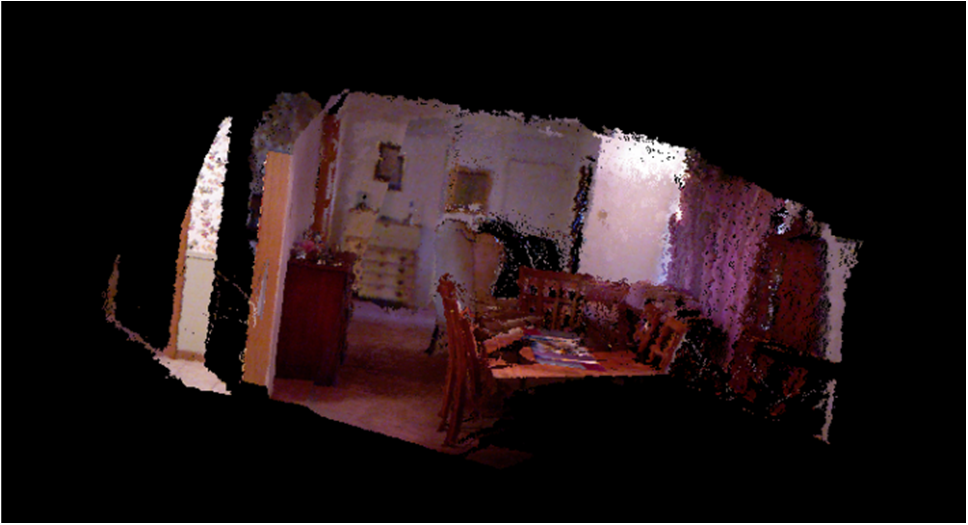
\includegraphics[width=3.2in ]{pics/pcl_stitch.png}
    \caption[Point cloud stitching map]{Point cloud stitching map~\cite{makhubela2023vslam}}\label{pcl_stitch}
\end{figure}

\noindent The study on the ROM20, an autonomous mobile robot platform for medical purposes, demonstrates
the use of modular designs and omni-directional movement through mecanum wheels~\cite{baskoro2020autonomous}.
The ROM20 can be equipped
with various subsystems, such as disinfectant sprayers, UVC lamps, and food delivery modules as demonstrated in \figref{bask}, hence it is versatile
for different medical tasks. However, mecanum wheels can be complex to control and lack in perfomance,
particularly on uneven or cluttered floors. This robot also only uses Bluetooth via a Teensy 4.0 microcontroller
making it limited to a short-range of 22 meters. In essence, ROM20 is not a fully autonomous robot, a 
lot of improvements can be made. 


\begin{figure}[H]
    \centering
    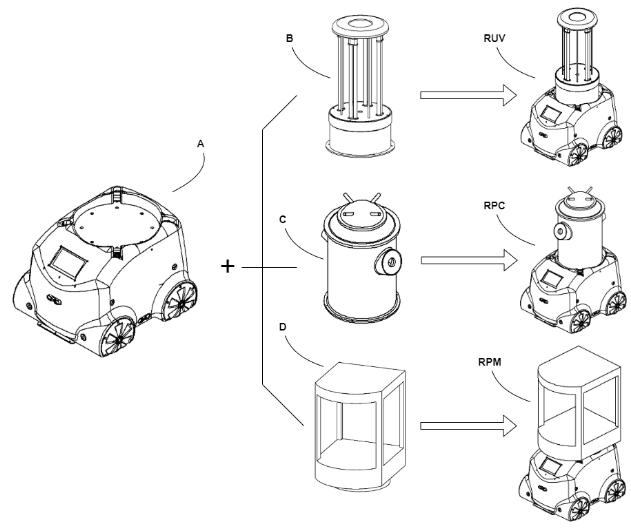
\includegraphics[width=3.8in ]{pics/modular_rom20.png}
    \caption[Modular sybsystems of ROM20]{Modular subsystems of ROM20~\cite{baskoro2020autonomous}}\label{bask}
\end{figure}

\subsubsection{Navigation with Hector SLAM and AMCL}
\noindent While still on the omnidirectional robots, ARIS 1.0 is an autonomous multitasking medicals service
robot that can be used in hospitals, particularly during pandemics~\cite{dunuwila2024aris}. ARIS 1.0 is equipped with a three-wheeled
omnidirectional mobile platform as shown in \figref{ar_1}, achieving three Degrees of Freedom (DOF) neck mechanism, and ROS-based
semi-autonomous navigation capabilities. It's unique features include a telepresence system, IoT-based
vital sign extraction, and the ability to communicate in regional languages, specifically Sinhala. The architecture of this robot was based on three parts; sensors, controllers, and Actuators. The main sensors were the 2D LiDAR, Camera, wheel encoders and a microphone. Three controllers were used; Jetson Nano for High level control which processed the sensor data and integrated it with how the display and speaker would 
function in the actuators part. The low level controllers are the Arduino Mega which controls the encoders and the motor controllers, 
and the Raspberry Pi 3B+ for Limit switches and mainly control the neck mechanism for the robot. As for navigation, Hector SLAM~\cite{nagla2020hector} is used for mapping and Adaptive Monte Carlo Localization (AMCL)~\cite{chung2022improved} is
applied for localization.
The robot was able to facilitate remote ward rounds and telemedicine. However, the ARIS 1.0 system's reliance on a
single 2D LiDAR for navigation poses challenges in case of a dynamic hospital setting which can have a complex
environment, since its precision is limited. 



\vspace{1.5em}

\begin{figure}[H]
    \centering
    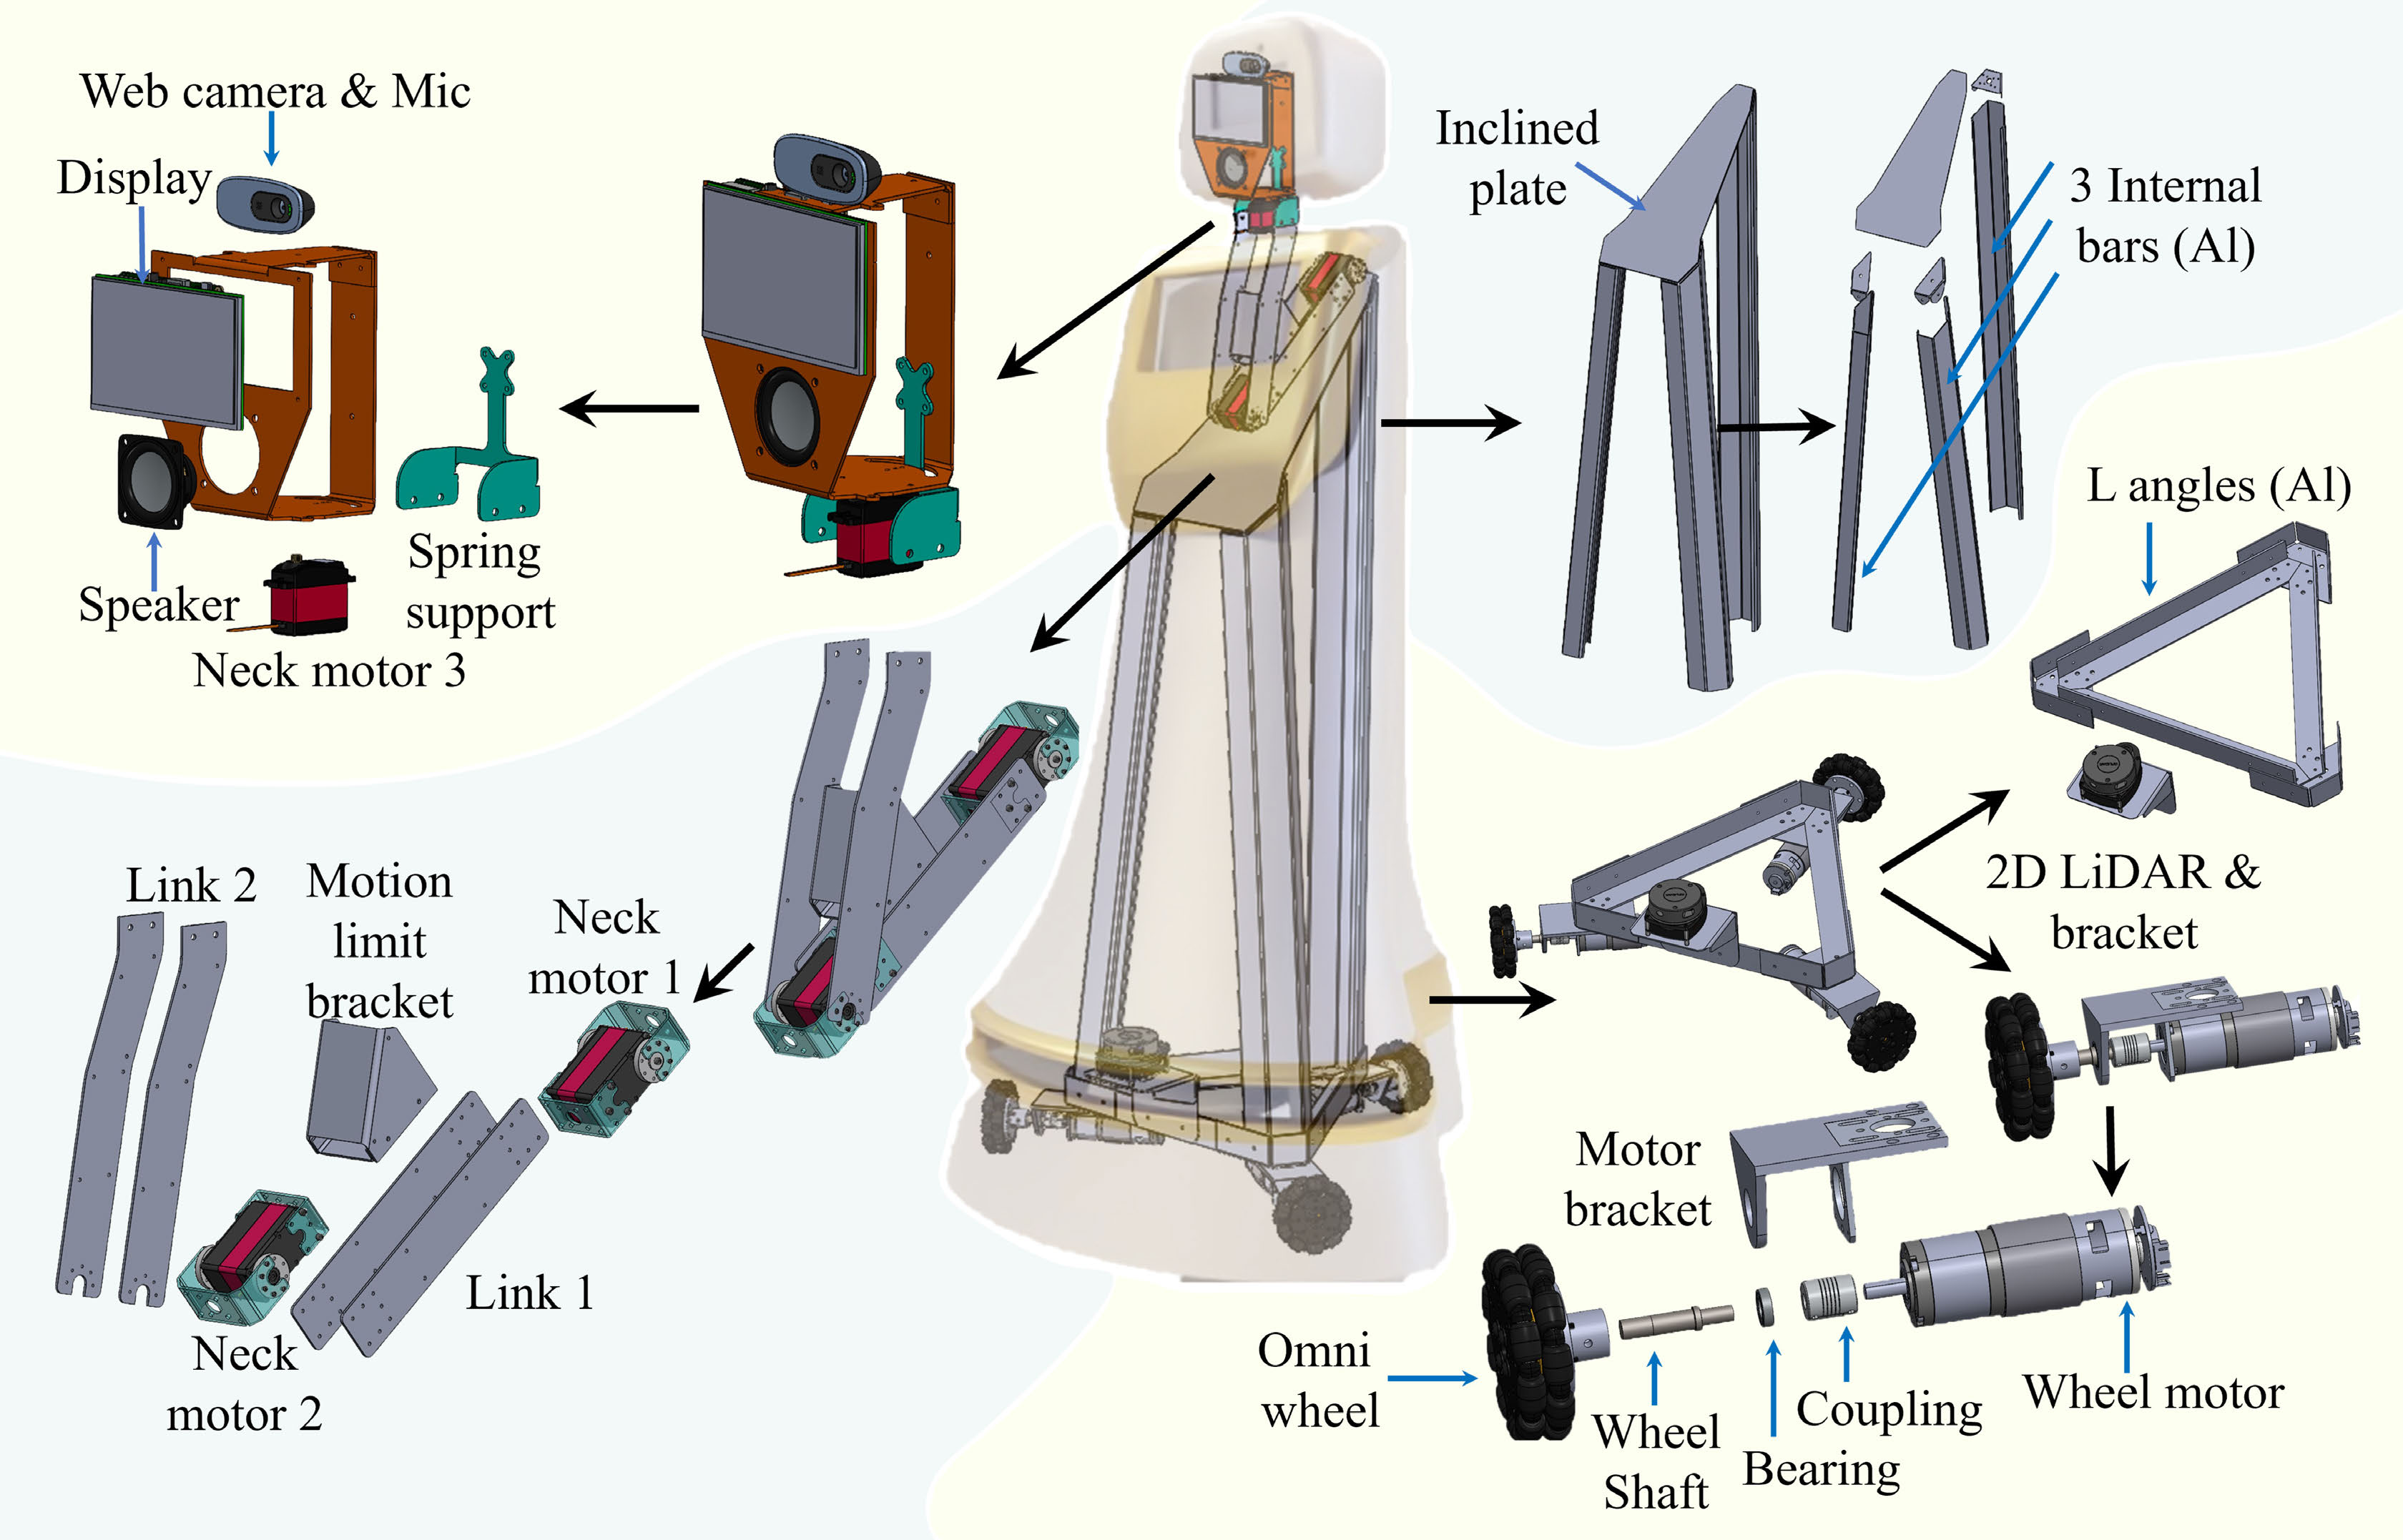
\includegraphics[width=5.5in ]{pics/explod_aris.png}
    \caption[Exploded view of ARIS 1.0]{Exploded view of ARIS 1.0~\cite{nagla2020hector}}\label{ar_1}
\end{figure}

\noindent Moreover, the study in~\cite{valner2022scalable} explores the use of autonomous robots to transport time-critical samples, such as
blood samples, from the Intensive Care Unit (ICU) to the laboratory in Tartu University Hospital. The robot's objective is to automate
non-medical task, such as transporting medical items, to free healthcare professionals from secondary duties, thus allowing more time focus
on patient care. The robot's were deployed using Robotics Middleware Framework (RMF)~\cite{quigley2020ros2}, an open-source fleet management
platform designed for coordinating and integrating fleets of robots within an existing building infrastructure like doors and elevators. 

\vspace{1.0em}
\begin{figure}[H]
    \centering
    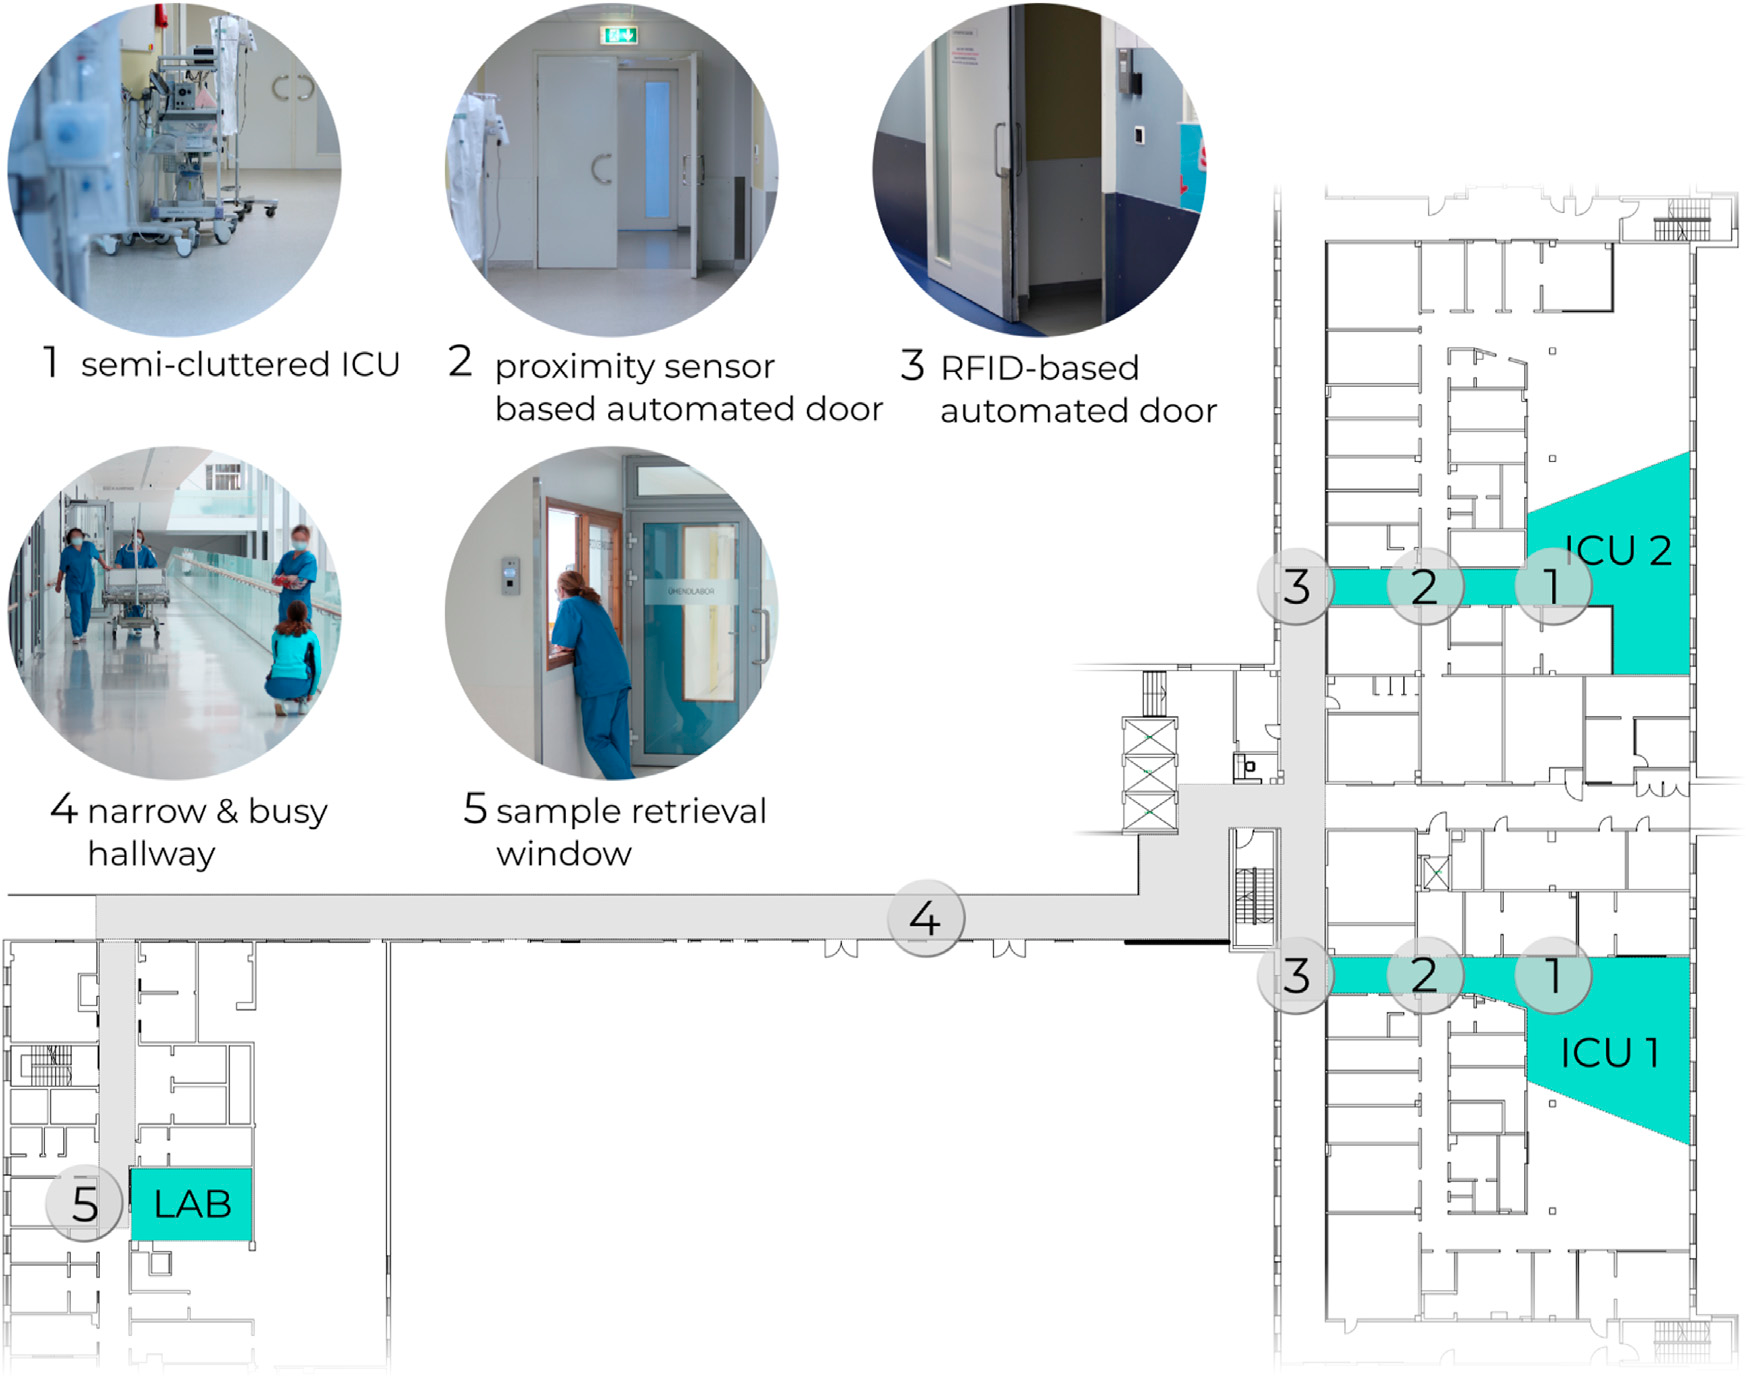
\includegraphics[width=5.5in]{pics/floor_tarta.png}
    \caption[Floorplan of Tarta University Hospital during object transportation]{Floorplan of Tarta University Hospital during object transportation~\cite{valner2022scalable}}\label{tarta1}
\end{figure} 

\vspace{-0.1em}

\noindent The use of RMF allowed for real-time task distribution, route planning, and system monitoring of the robots. RMF system was built as a
distributed application using ROS2 nodes. The nodes communicate through ROS2 topics and services, and the Data Distribution Service (DDS) protocol
allows real-time communication between the robots and the RMF system. Most importantly, navigation commands and robot status are sent via topics and
services.\@ Since RMF has the hospital infrastructure, custom ROS2 nodes were developed to control door mechanisms via commands received from the RMF.\@
An example is given where a ROS2 node running on a Raspberry Pi is connected to the door controllers and activated the servo motors that
opened the doors upon receiving commands from the RMF.\@ 


\begin{figure}[H]
    \centering
    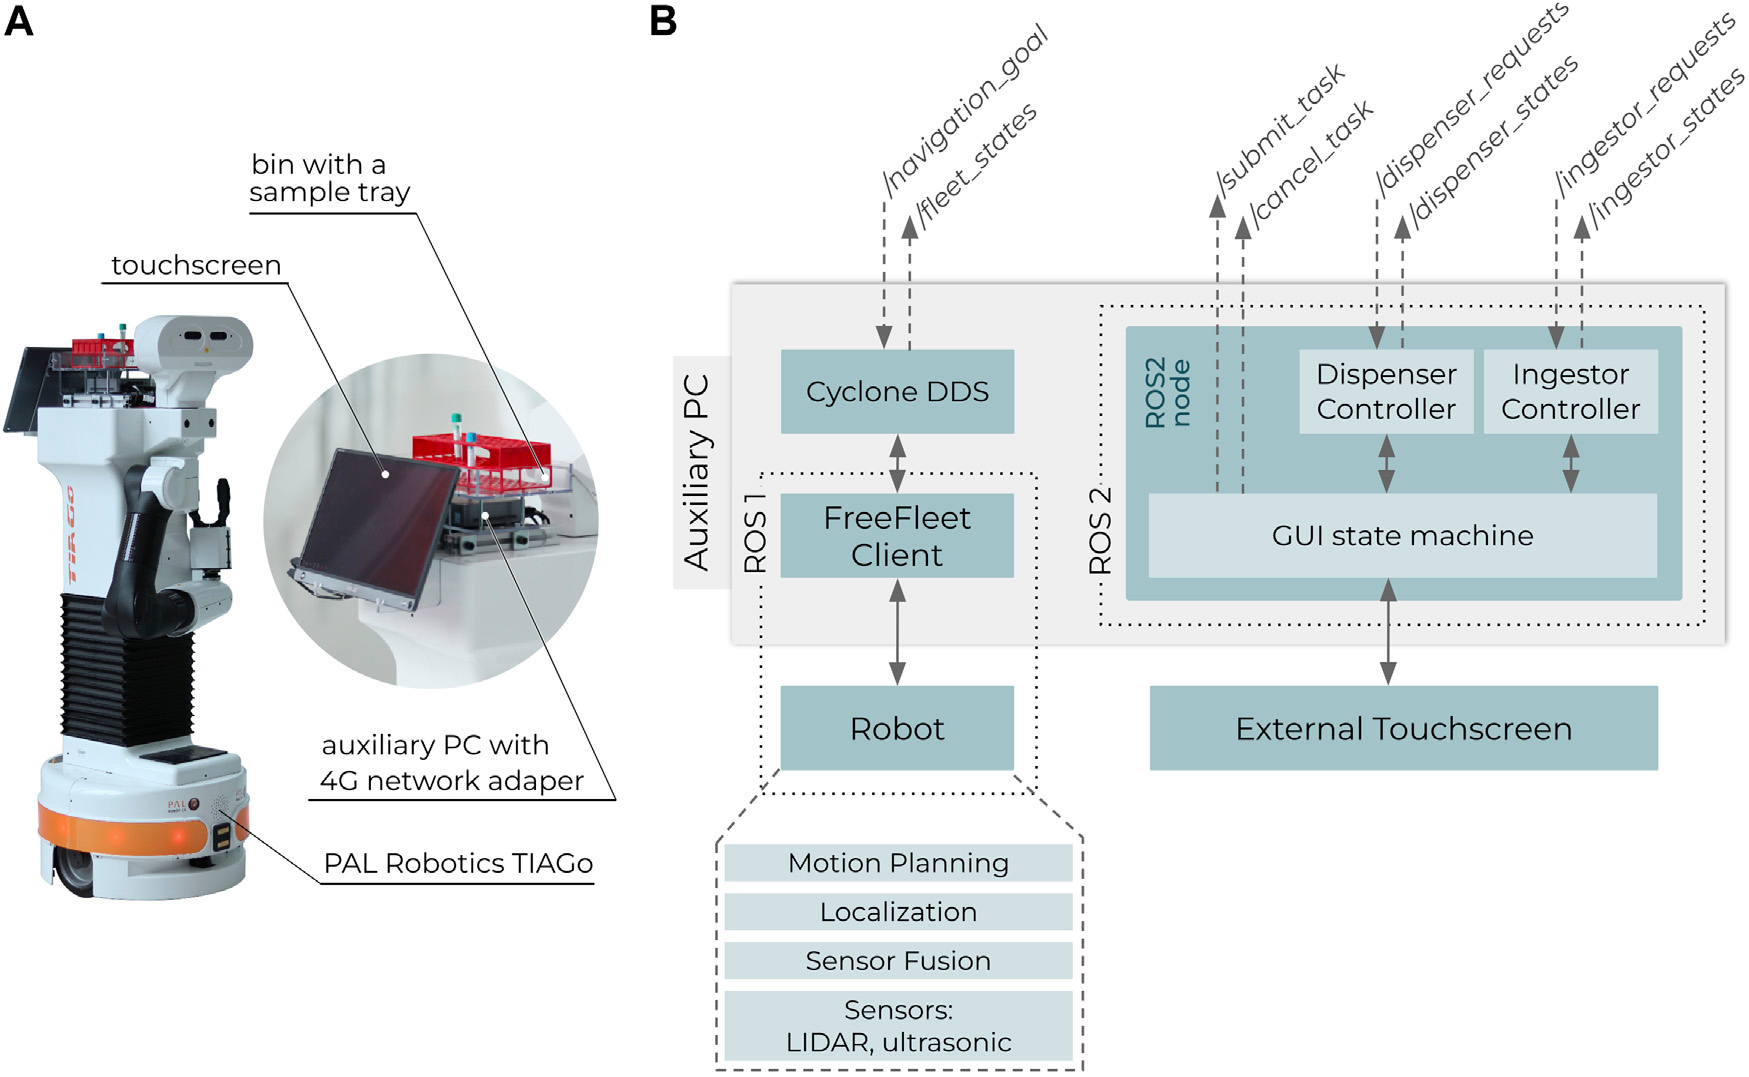
\includegraphics[width=4.5in]{pics/rmf2.png}
    \caption[PAL Robotics TIAGo hardware \textbf{(A)}. Software setup of the whole robot \textbf{(B)}.]{PAL Robotics TIAGo hardware \textbf{(A)}. Software setup of the whole robot \textbf{(B)}.~\cite{valner2022scalable}}\label{stm32_pi}
\end{figure}





\subsection{Summary of the literature review}
The literature emphasizes that effective robot navigation hinges on four key components: perception, localization, cognition, and motion control. Perception involves acquiring environmental data through sensors such as cameras, LiDAR, and ultrasonic sensors. Localization determines the robot's position within the environment, while cognition focuses on path planning and obstacle avoidance decision-making processes. Motion control translates these decisions into motor commands to execute navigation tasks.
Various localization and mapping techniques have been explored to enhance navigation accuracy. Dead reckoning provides position estimates based on previous movements but is prone to cumulative errors. Kalman Filters (KF) and Extended Kalman Filters (EKF) offer probabilistic approaches for state estimation and handling of linear and nonlinear systems. However, they require accurate models and may need to cope better with complex environments. Particle Filters, such as Monte Carlo Localization (MCL) and its adaptive variant AMCL, represent the robot's belief state with weighted particles, accommodating non-linearities and non-Gaussian noise, making them suitable for dynamic settings.
Algorithms like Grid-based FastSLAM (Gmapping) and Hector SLAM are used for mapping. Gmapping builds occupancy grid maps in real-time, which is ideal for indoor environments. At the same time, Hector SLAM relies on high-frequency LiDAR data without requiring odometry, which is beneficial for robots lacking wheel encoders.
Path planning algorithms are crucial for safe and efficient navigation. The A* algorithm, an enhancement of Dijkstra's algorithm, introduces heuristics to expedite the search for optimal paths, balancing efficiency and computational demands. The Dynamic Window Approach (DWA) serves as a local planner, generating feasible velocity commands by considering the robot's dynamics, which is essential for navigating dynamic environments like hospital corridors.
The Robot Operating System 2 (ROS2) and its Navigation 2 Stack (Nav2) provide a robust framework for integrating these algorithms. Nav2's modular architecture allows for customization and seamless incorporation of various navigation strategies, leveraging ROS2's enhanced communication and real-time capabilities. Alternative frameworks like ARC Nav and RTAB-Map offer extended functionalities but may be unnecessarily complex or resource-intensive for ground-based robots in structured environments.
Considering related works, robots employing Gmapping and AMCL have demonstrated reliable navigation in hospital settings, with additional studies highlighting the benefits of sensor fusion using devices like RGB-D cameras for improved environmental perception. However, computational efficiency remains a concern, especially for real-time applications on resource-limited hardware.

\subsubsection*{Selection of Algorithms for the Project}

Based on the literature and the project objectives—developing an autonomous robot for medicine dispensing in hospital wards—the following algorithms have been selected:

\noindent\textbf{Localization and Mapping:} 
\begin{itemize}
    \item Adaptive Monte Carlo Localization (AMCL) \\
    \textit{Justification:} AMCL offers robust localization with dynamic particle adjustment, balancing accuracy and computational load, which is suitable for the Raspberry Pi 4. Gmapping is chosen for creating occupancy grid maps essential for indoor navigation.
\end{itemize}

\noindent\textbf{Path Planning:}
\begin{itemize}
    \item \textbf{Global Planner:} A* Algorithm. \\
    \textit{Justification:} A* efficiently computes optimal paths using heuristics, ensuring timely and effective route planning.
    \item \textbf{Local Planner:} Dynamic Window Approach (DWA).\\
    \textit{Justification:} DWA provides real-time obstacle avoidance by considering the robot's dynamics, which is essential for navigating dynamic environments like hospital corridors.
\end{itemize}







\begin{comment}

\begin{figure}[H]
    \centering
    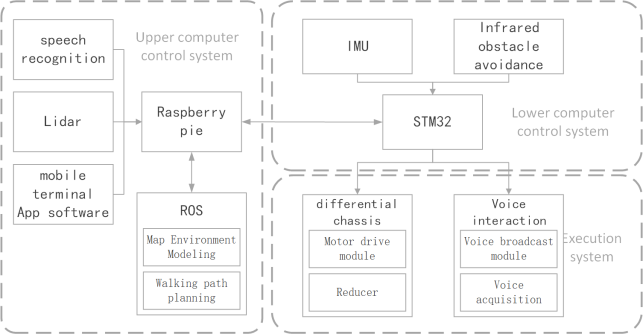
\includegraphics[width=4.8in ]{pics/stm32_pi.png}
    \caption{Composition block diagram of the entire system~\cite{kok2020intelligent}}
    \label{stm32_pi}
\end{figure}


\subsection{Summary of the literature review}

\end{comment}
%\newpage

\section{Methodology}

\subsection{Conceptual Design}

\subsubsection{Robot Chassis}
In mobile robots, there is a wide of range of chassis mechanism and differential types of wheels including mecanum wheels, omni and caster wheels.
The chassis is assembled using 20$\times$20 mm T-slot aluminum frame due to its strength-weight-ratio and modularity. The wheels are 150 mm in diameter
and pneumatic.

\begin{figure}[H]
    \centering
    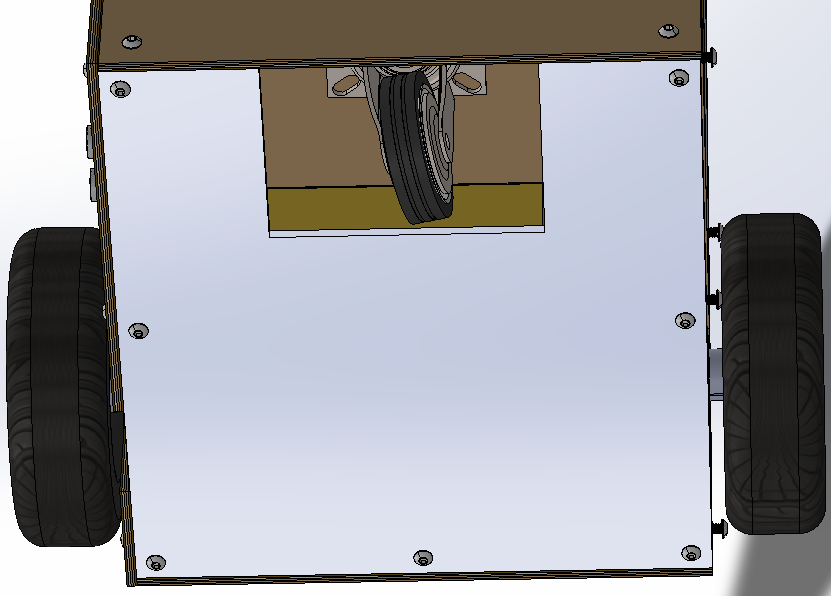
\includegraphics[width=5.5in]{pics/diff.png} 
    \caption{Differential drive chassis}\label{diff_cart}
\end{figure}

\noindent The robot has multiple compartments for medicine storage and delivery purposes. The height of the robot is 450mm, but will be reduced to
optimize costs. There are two layers: the lower layer houses the low-level actuators including motor drivers, motors, and battery,
while the upper layer contains the Single Board Computer (SBC) and Microcontroller Unit (MCU). A LiDAR sensor is mounted on the topmost 
section of the robot. The robot is enclosed with plywood panels attached to the 20$\times$20mm aluminum frame profiles. Emergency
stop buttons are positioned on the rear of the robot, and a switch will be mounted on the front panel to confirm delivery.

\begin{figure}[H]
    \centering
    \begin{minipage}{0.45\textwidth}
        \centering
        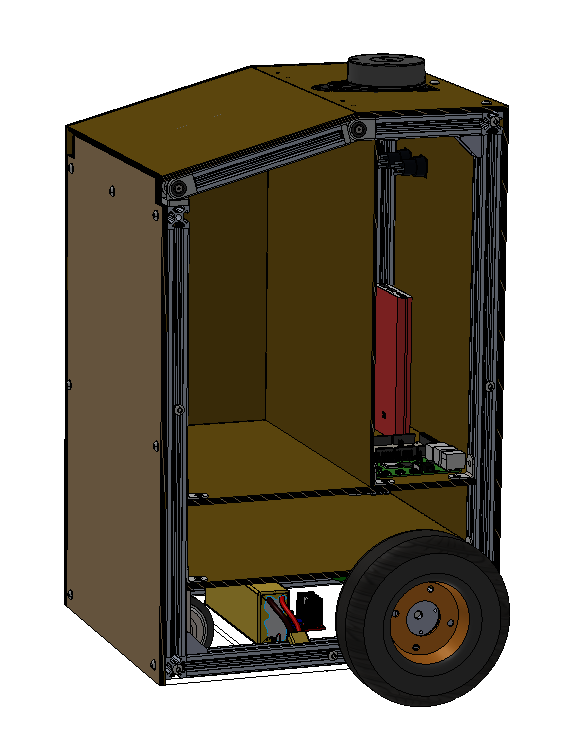
\includegraphics[width=2.9in]{pics/front_cart.png}
    \end{minipage}\hfill
    \begin{minipage}{0.45\textwidth}
        \centering
        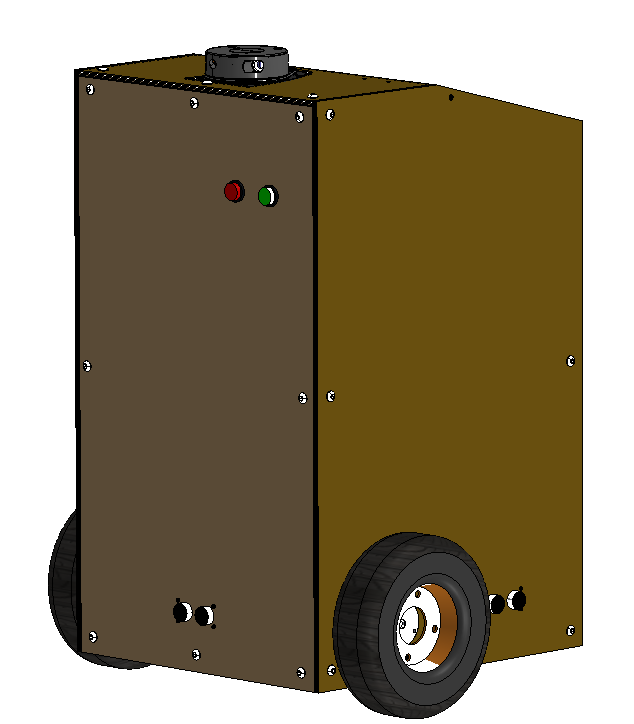
\includegraphics[width=2.9in]{pics/back_cart.png}
    \end{minipage}\hfill
    \caption{Isometric views of the robot}\label{back_cart}
\end{figure}

\vspace{-1.2em}

\subsubsection{Kinematic Model}
For this project, there are two independent driving wheels which are equipped with either one or two passive wheel(s) of caster type. The wheels
can turn at different speeds and they are attached to the robot on the same axis hence they can govern the direction of movement of the robot
as well as its speed. The wheels have radius $r$, separated by a wheelbase of length $L = 2b$, where $b$ is half the distance between the wheels. The robot's motion is controlled by varying the angular velocities of the left and right wheels, denoted by $\dot{\theta}_l$ and $\dot{\theta}_r$, respectively.

\begin{figure}[H]
    \begin{minipage}{0.55\textwidth}
        \begin{enumerate}[label=\alph*)]
            \item Equal speed in both wheels = forward motion
            \item Equal speed in both wheels = backward motion
            \item Equal speed in both wheels, but in opposite\\ directions
            \item Higher speed for left wheel = robot turns right
            \item Higher speed for right wheel = robot turns left
        \end{enumerate}
    \end{minipage}
    \hfill
    \begin{minipage}{0.45\textwidth}
        \centering
        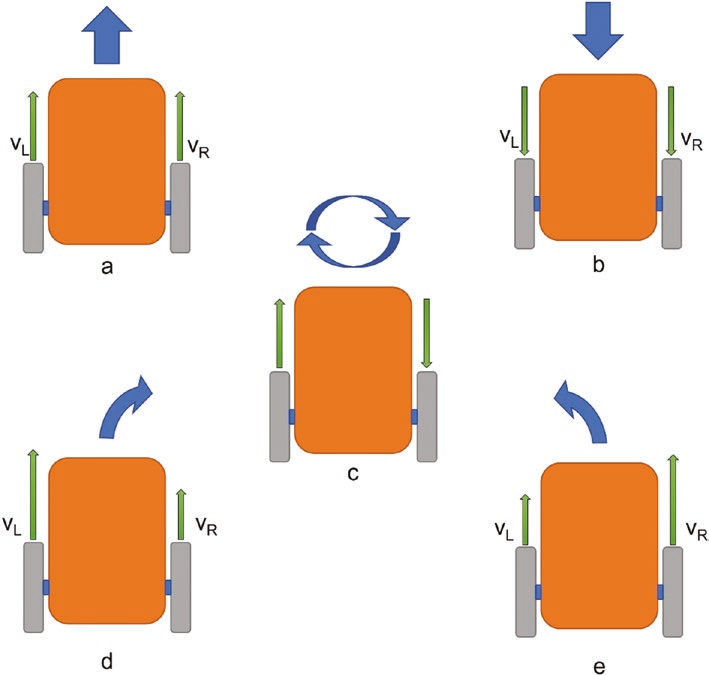
\includegraphics[width=1.7in]{pics/kine.png}
        \caption[Motion description of a two-wheel differential drive chassis]{Visual description~\cite{subramanian2023autonomous}}
        \label{kine1}
    \end{minipage}
\end{figure}

\vspace{-1em}

\noindent Two coordinate frames are defined to describe the robot's motion:

\vspace{-0.8em}

\begin{enumerate} 
    \setlength\itemsep{-0.5em}
    \item \textbf{Inertial Frame} $(X, Y)$: A global, fixed reference frame. 
    \item \textbf{Body Frame} $(x, y)$: A frame attached to the robot, with the $x$-axis pointing forward and the $y$-axis pointing to the left. 
\end{enumerate}


\begin{figure}[H]
    \centering
    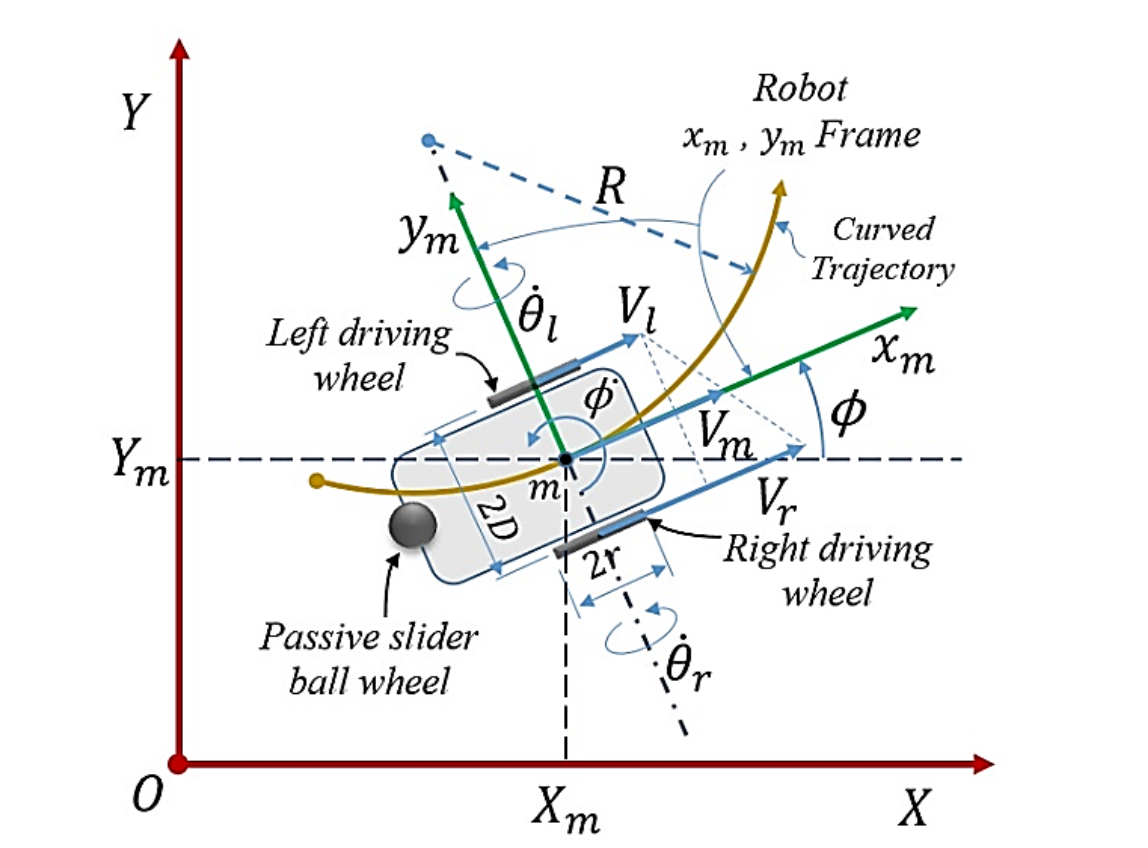
\includegraphics[width=4.0in]{pics/x_y.png}
    \caption[Kinematic structure of a differential drive]{Kinematic structure of a differential drive~\cite{azevedo2018lidar}}
\end{figure} 


\noindent The robot's pose in the inertial frame is represented by the vector $\mathbf{p} = [X_m, Y_m, \phi]^\top$, where $X_m$ and
$Y_m$ are the position coordinates, and $\phi$ is the orientation angle between the robot's heading and the inertial $X$-axis. Assumptions are taken into consideration that the robot wheels are rolling without slipping and the centre of mass of the robot is
located at the axis of the wheels rotation. Under the no-slfip assumption (i.e., the wheels roll without lateral slipping), the
robot's instantaneous motion in its body frame can be described by:

\vspace{-0.25em}

\begin{equation} \begin{aligned} \dot{x} &= v, \ \dot{y} &= 0, \ \dot{\phi} &= \omega, \end{aligned} \end{equation}

where:

\begin{itemize}
    \setlength\itemsep{-0.5em}
    \item $v$ is the linear velocity along the robot's forward direction ($x$-axis),
    \item $\omega$ is the angular velocity around the vertical axis (rotation rate),
    \item $\dot{x}$ and $\dot{y}$ are the velocities along the $x$ and $y$ axes of the body frame,
    \item $\dot{\phi}$ is the rate of change of the robot's orientation,
    \item \( r \) be the radius of each wheel,
    \item \( L = 2b \) be the wheelbase (the distance between the two wheels),
    \item \( \dot{\theta}_l \) and \( \dot{\theta}_r \) be the angular velocities of the left and right wheels, respectively.
\end{itemize}


\noindent For motion analysis, the robot’s linear velocity \( v \) and angular velocity \( \omega \) about its center are given by:

\begin{equation}
v = \frac{r}{2} \left( \dot{\theta}_r + \dot{\theta}_l \right)
\label{eq:linear_velocity}
\end{equation}

\vspace{-0.25em}

\begin{equation}
\omega = \frac{r}{L} \left( \dot{\theta}_r - \dot{\theta}_l \right)
\label{eq:angular_velocity}
\end{equation}


\noindent For velocity analysis, the condition $\dot{y} = 0$ arises because, in the body frame, the robot cannot move sideways without wheel slippage. The wheels can only induce motion along the forward direction and rotation about the robot's center.
The velocities \( \dot{X} \), \( \dot{Y} \), and \( \dot{\phi} \) in the inertial frame are related to the body frame velocities \( v \) and \( \omega \) by:

\begin{equation}
\begin{bmatrix} \dot{X} \\ \dot{Y} \\ \dot{\phi} \end{bmatrix}
=
\begin{bmatrix} \cos \phi & 0 \\ \sin \phi & 0 \\ 0 & 1 \end{bmatrix}
\begin{bmatrix} v \\ \omega \end{bmatrix}
\label{eq:transformation}
\end{equation}


\noindent Transfomring the velocities from the body frame to the inertial frame gives

\begin{equation}
    \begin{bmatrix} \dot{X} \\ \dot{Y} \\ \dot{\phi} \end{bmatrix}
    =
    \begin{bmatrix} v\cos \\v\sin \\ \omega \end{bmatrix}
    \label{eq:transformation2}
\end{equation}
    



\noindent Using wheel encoders, the angular velocities \( \dot{\theta}_l \) and \( \dot{\theta}_r \) can be approximated as:

\begin{equation}
\dot{\theta}_l = \frac{\Delta \theta_l}{\Delta t}, \quad \dot{\theta}_r = \frac{\Delta \theta_r}{\Delta t}
\label{eq:encoder_velocities}
\end{equation}

\noindent where \( \Delta \theta_l \) and \( \Delta \theta_r \) are the incremental angular
displacements of the left and right wheels over the sampling interval \( \Delta t \).Substituting
Equation~\eqref{eq:encoder_velocities} into Equations~\eqref{eq:linear_velocity} 
and \eqref{eq:angular_velocity} yields the following:

\begin{equation}
v = \frac{r}{2 \Delta t} \left( \Delta \theta_r + \Delta \theta_l \right)
\label{eq:linear_velocity_encoder}
\end{equation}

\begin{equation}
\omega = \frac{r}{L \Delta t} \left( \Delta \theta_r - \Delta \theta_l \right)
\label{eq:angular_velocity_encoder}
\end{equation}

\noindent These equations allow computation of the robot's linear and angular velocities based on encoder data.


\newpage
\subsection{Hardware Implementation}



\subsubsection{Sensors design specifications}
For this section, the sensors to be used in the robot are analysed and their specifications are presented while determining the proper placement of each of the sensor element on the robot. 
As sensors' workings, their algorithms and how they interact, this will be further discussed in the software implementation section. 
To achieve navigation, one of the most popular sensors used is the LiDAR. 



\begin{table}[h]
    \begin{minipage}{0.5\textwidth}
    \centering
    \renewcommand{\arraystretch}{2.0}
    \setlength{\tabcolsep}{4.4pt}
    \footnotesize
    \begin{tabular}{|p{3cm}|p{4.4cm}|}
      \hline
      \rowcolor[gray]{0.8} 
      \textbf{Parameter} & \textbf{Value} \\
      \hline
      Measuring Range & 0.15m - 12m \\
      \hline
      Rotational Speed & 5.5Hz \\
      \hline
      Scanning Angle & 360$^{\circ}$ \\
      \hline
      Scanning Frequency & 10Hz \\
      \hline
      System Voltage & 5V \\
      \hline
      System Current & 100mA \\
      \hline
      Dimensions & 96.8mm x 70.3mm x 55mm \\
      \hline
      Sampling frequency & 8K \\      
      \hline
      Angular Resolution & $\leq 1^{\circ}$ \\
      \hline
      Output & UART Serial (3.3V) \\
      \hline
      Temperature Range & 0$^{\circ}$C - 40$^{\circ}$C \\
      \hline
      Range Resolution & $\leq 1\%$ of the range ($\leq 12m$), $\leq 2\%$ of the range (12m - 16m) \\
      \hline
    \end{tabular}
    \end{minipage}
    \begin{minipage}{0.55\textwidth}
        \centering
        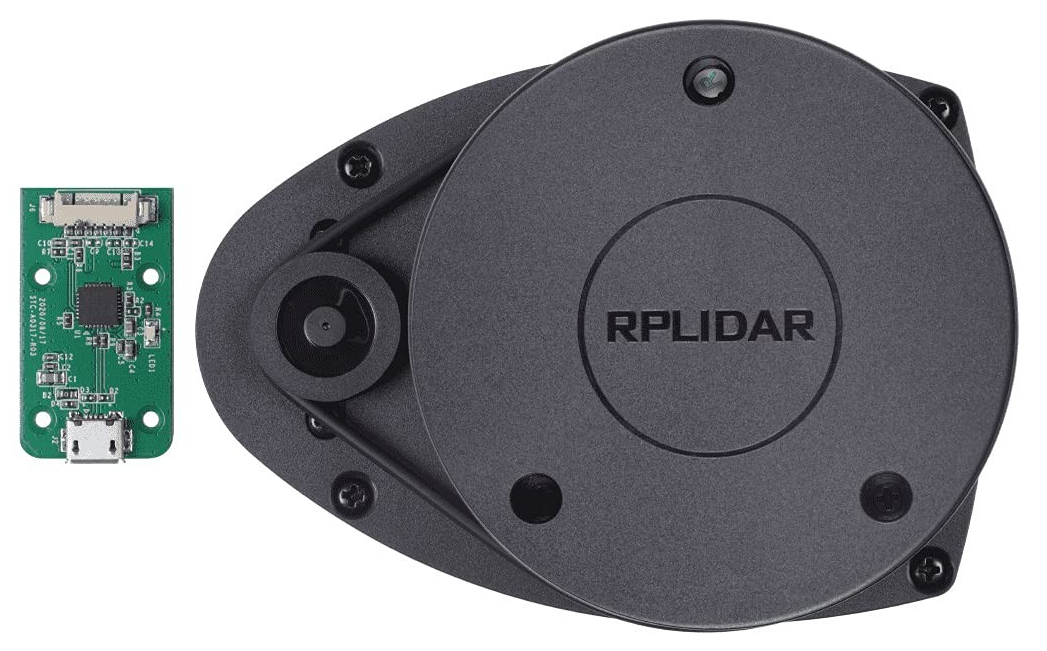
\includegraphics[width=\linewidth, angle=90]{pics/lidar.png}
    \end{minipage}\hfill
    \caption{RPLiDAR A1 M8 and its basic operating parameters}\label{tab:lidar}
\end{table}



\noindent RP LiDAR A1 M8 as shown in \figref{tab:lidar} is a 2D LiDAR sensor that performs 360-degree scanning with a range of 12 meters.
The sensor will be connected to the Raspberry Pi 4 via USB and powered by a 5V supply from the buck converter. LiDARs typically have a vertical measurement range~\cite{azevedo2018lidar}, thus requires it
placed at a certain height to avoid obstacles from the robot's side covers or the ground. To ensure this is achieved the LiDAR will be mounted on a 3D printed bracket that is attached on top of the robot at a 
450mm height.

\vspace{1.0em}
\begin{figure}[H]
    \centering
    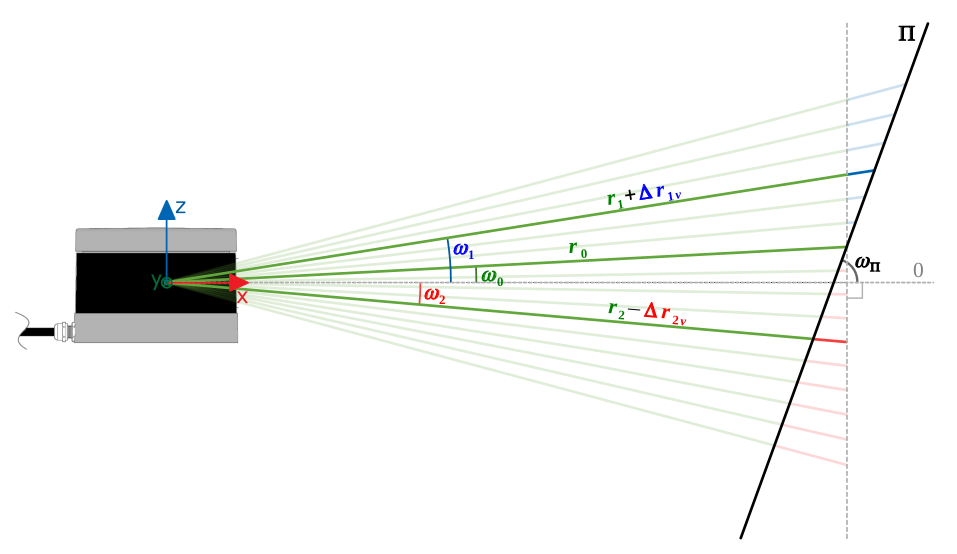
\includegraphics[width=3.8in]{pics/vertical.png}
    \caption[Vertical measurement of a LiDAR]{Vertical measurements of a LiDAR~\cite{azevedo2018lidar}}\label{vert}
\end{figure} 


\noindent For more safety on the autonomous navigation, it should also be accessible from obstacles throughout the horizontal plane to maximize its field of view. 
Thus incorporating ultrasonic sensors, Time of Flight sensor and IMU is essential so as to achieve fault-tolerant redundancy that helps other sensors~\cite{CANADASARANEGA2024100606}.
Ultrasonic sensors used high-frequency sound waves to detect objects around the the robot's perimeter. HC-SR04 is a popular ultrasonic sensor that has a range of 2cm to 400cm.
VL53L0X is a Time of Flight sensor that uses a laser to measure the distance between the robot and an object. It has a range of up to 2 meters. This sensor will be placed 
in front of the robot bumper while the three ultrasonics will be mounted on sides and the robot's rear. The Inertial Measurement Unit (IMU) integrates three types of sensors into a single
device: accelerometer, gyroscope, and a magnetometer. MPU-9250 is a popular IMU chosen for this project. It is 9-DOF meaning the sensor can measure in three-axis; acceleration (x,y,z), angular velocity (roll, pitch, yaw), and magnetic field(x,y,z).
The main reason why the IMU is used is to provide the robot with orientation and position data, that maintain accuracy of localization on robot thus making it much smoother.


\vspace{1.0em}

\begin{figure}[H]
    \centering
    \begin{minipage}{0.3\textwidth}
        \centering
        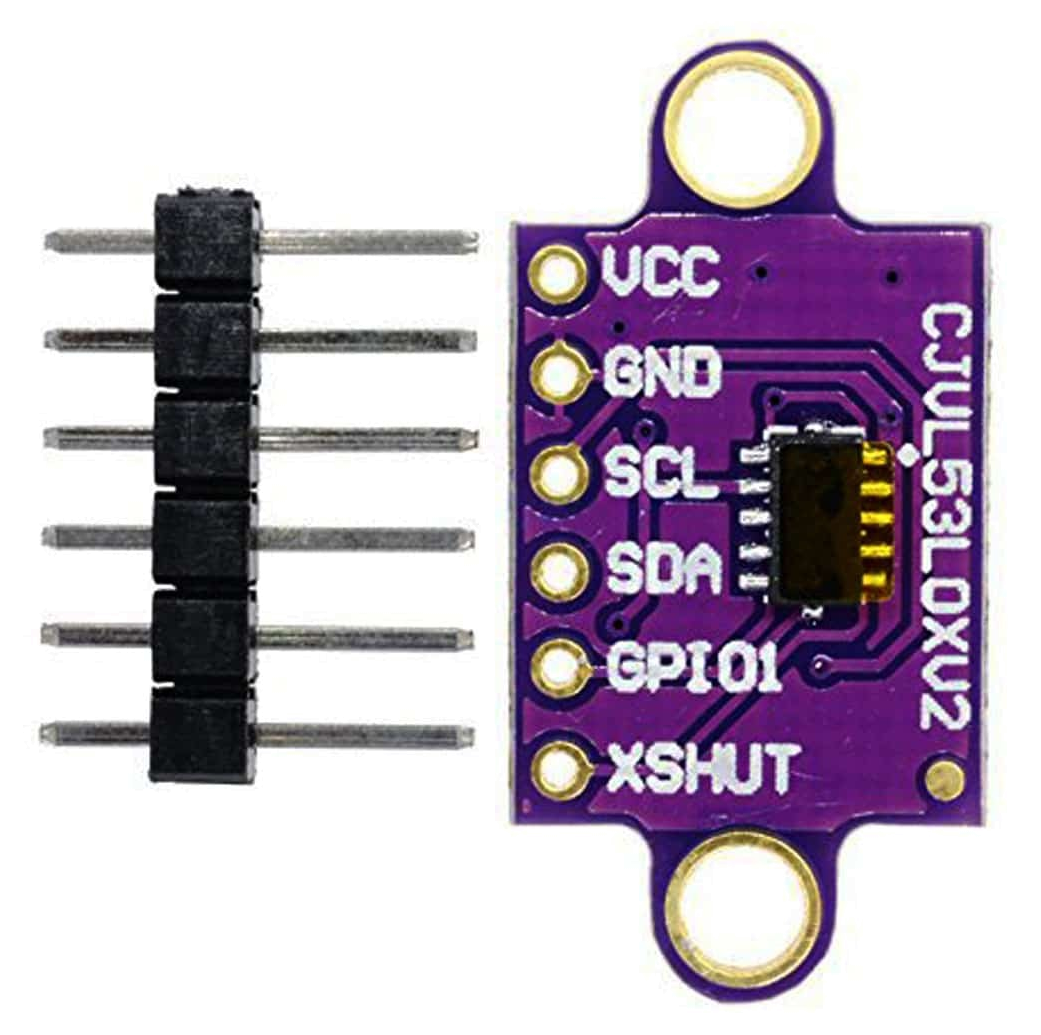
\includegraphics[width=\linewidth]{pics/tof.png}
        \caption{Time of Flight}\label{tof}
    \end{minipage}\hfill
    \begin{minipage}{0.3\textwidth}
        \centering
        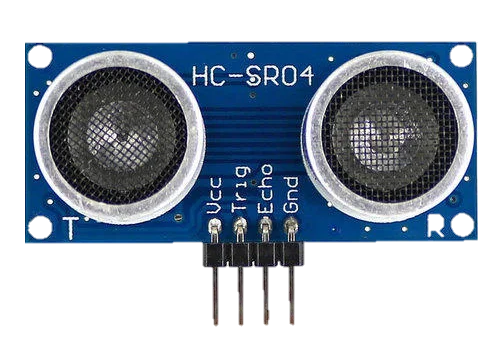
\includegraphics[width=\linewidth]{pics/hcrs04.png}
        \caption{HCR-S04}\label{ultra}
    \end{minipage}\hfill
    \begin{minipage}{0.3\textwidth}
        \centering
        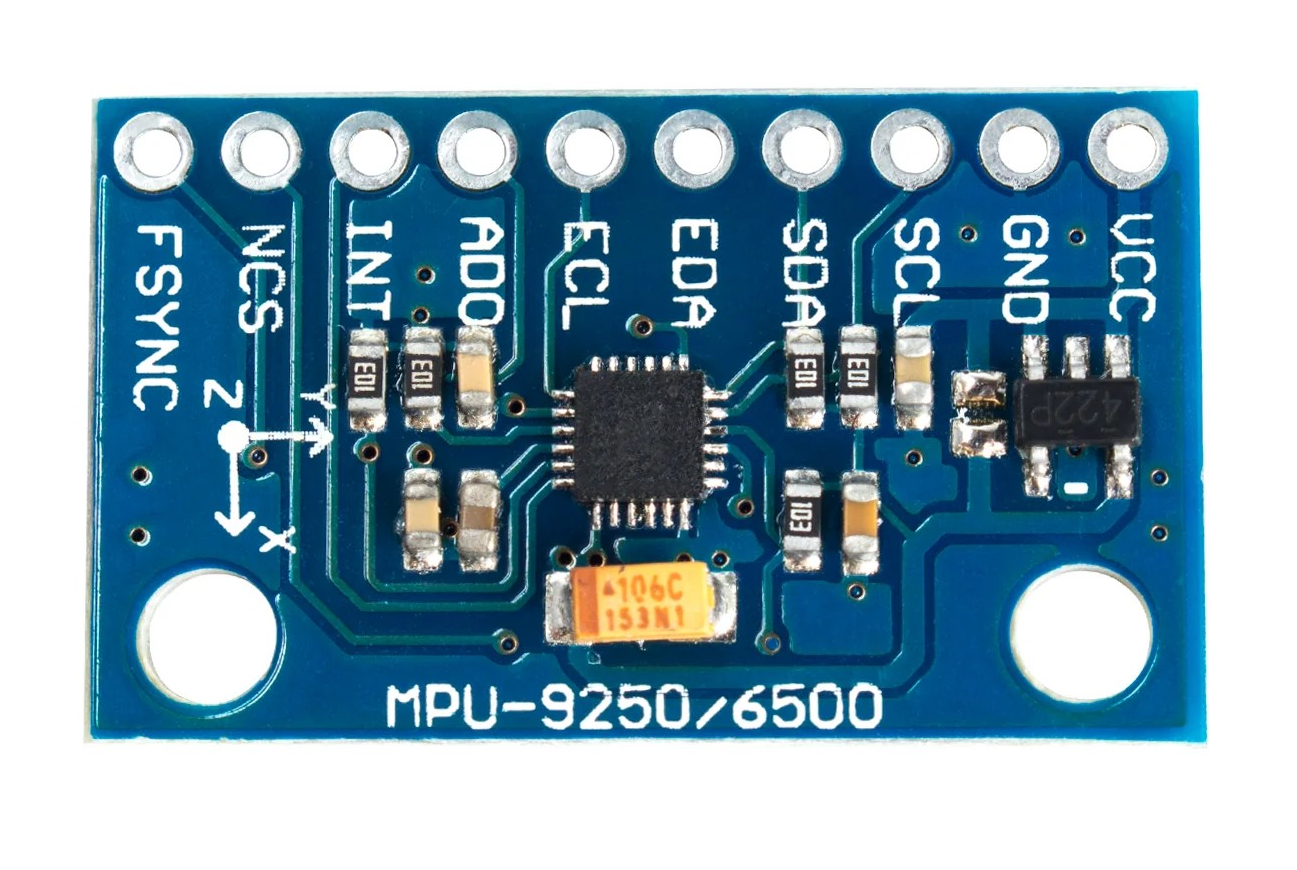
\includegraphics[width=\linewidth]{pics/mpu.png}
        \caption{MPU-9250 IMU}\label{mpu}
    \end{minipage}
    \caption{Proximity sensors used in the project}\label{prox}
    \label{fig:lidar_side_by_side}
\end{figure}

\newpage


\subsubsection{Onboard Computer}

\vspace{-0.8em}

A Raspberry Pi 4 is chosen as the onboard computer for this project, working alongside an ESP32 microcontroller. While the Raspberry Pi handles high-level processing and navigation tasks, the ESP32 is responsible for low-level control functions including motor control and sensor interfacing.

\begin{table}[h]
    \begin{minipage}{0.6\textwidth}
        \centering
        \renewcommand{\arraystretch}{2.0}
        \setlength{\tabcolsep}{4.4pt}
        \footnotesize
        \begin{tabular}{|p{2.9cm}|p{6.4cm}|}
          \hline
          \rowcolor[gray]{0.8} 
          \textbf{Parameter} & \textbf{Value} \\
          \hline
          SoC & Broadcom BCM2711, Cortex-A72 (ARM v8) 64-bit SoC @ 1.8GHz \\
          \hline
          Memory & 8GB LPDDR4-3200 SDRAM (micro SD card slot) \\
          \hline
          Wireless & 2.4 GHz and 5.0 GHz IEEE 802.11ac wireless, Bluetooth 5.0, BLE \\
          \hline
          Audio/Video & 4-pole stereo audio and composite video port \\
          \hline
          Video & H.265 (4kp60 decode) \newline H264 (1080p60 decode, 1080p30 encode) \\
          \hline
          Power Supply & 5VDC, 3A, Power over Ethernet (PoE) \\
          \hline
          Temperature Range & 0 – 50 $^\circ$C ambient \\
          \hline
        \end{tabular}
    \end{minipage}
    \begin{minipage}{0.47\textwidth}
        \centering
        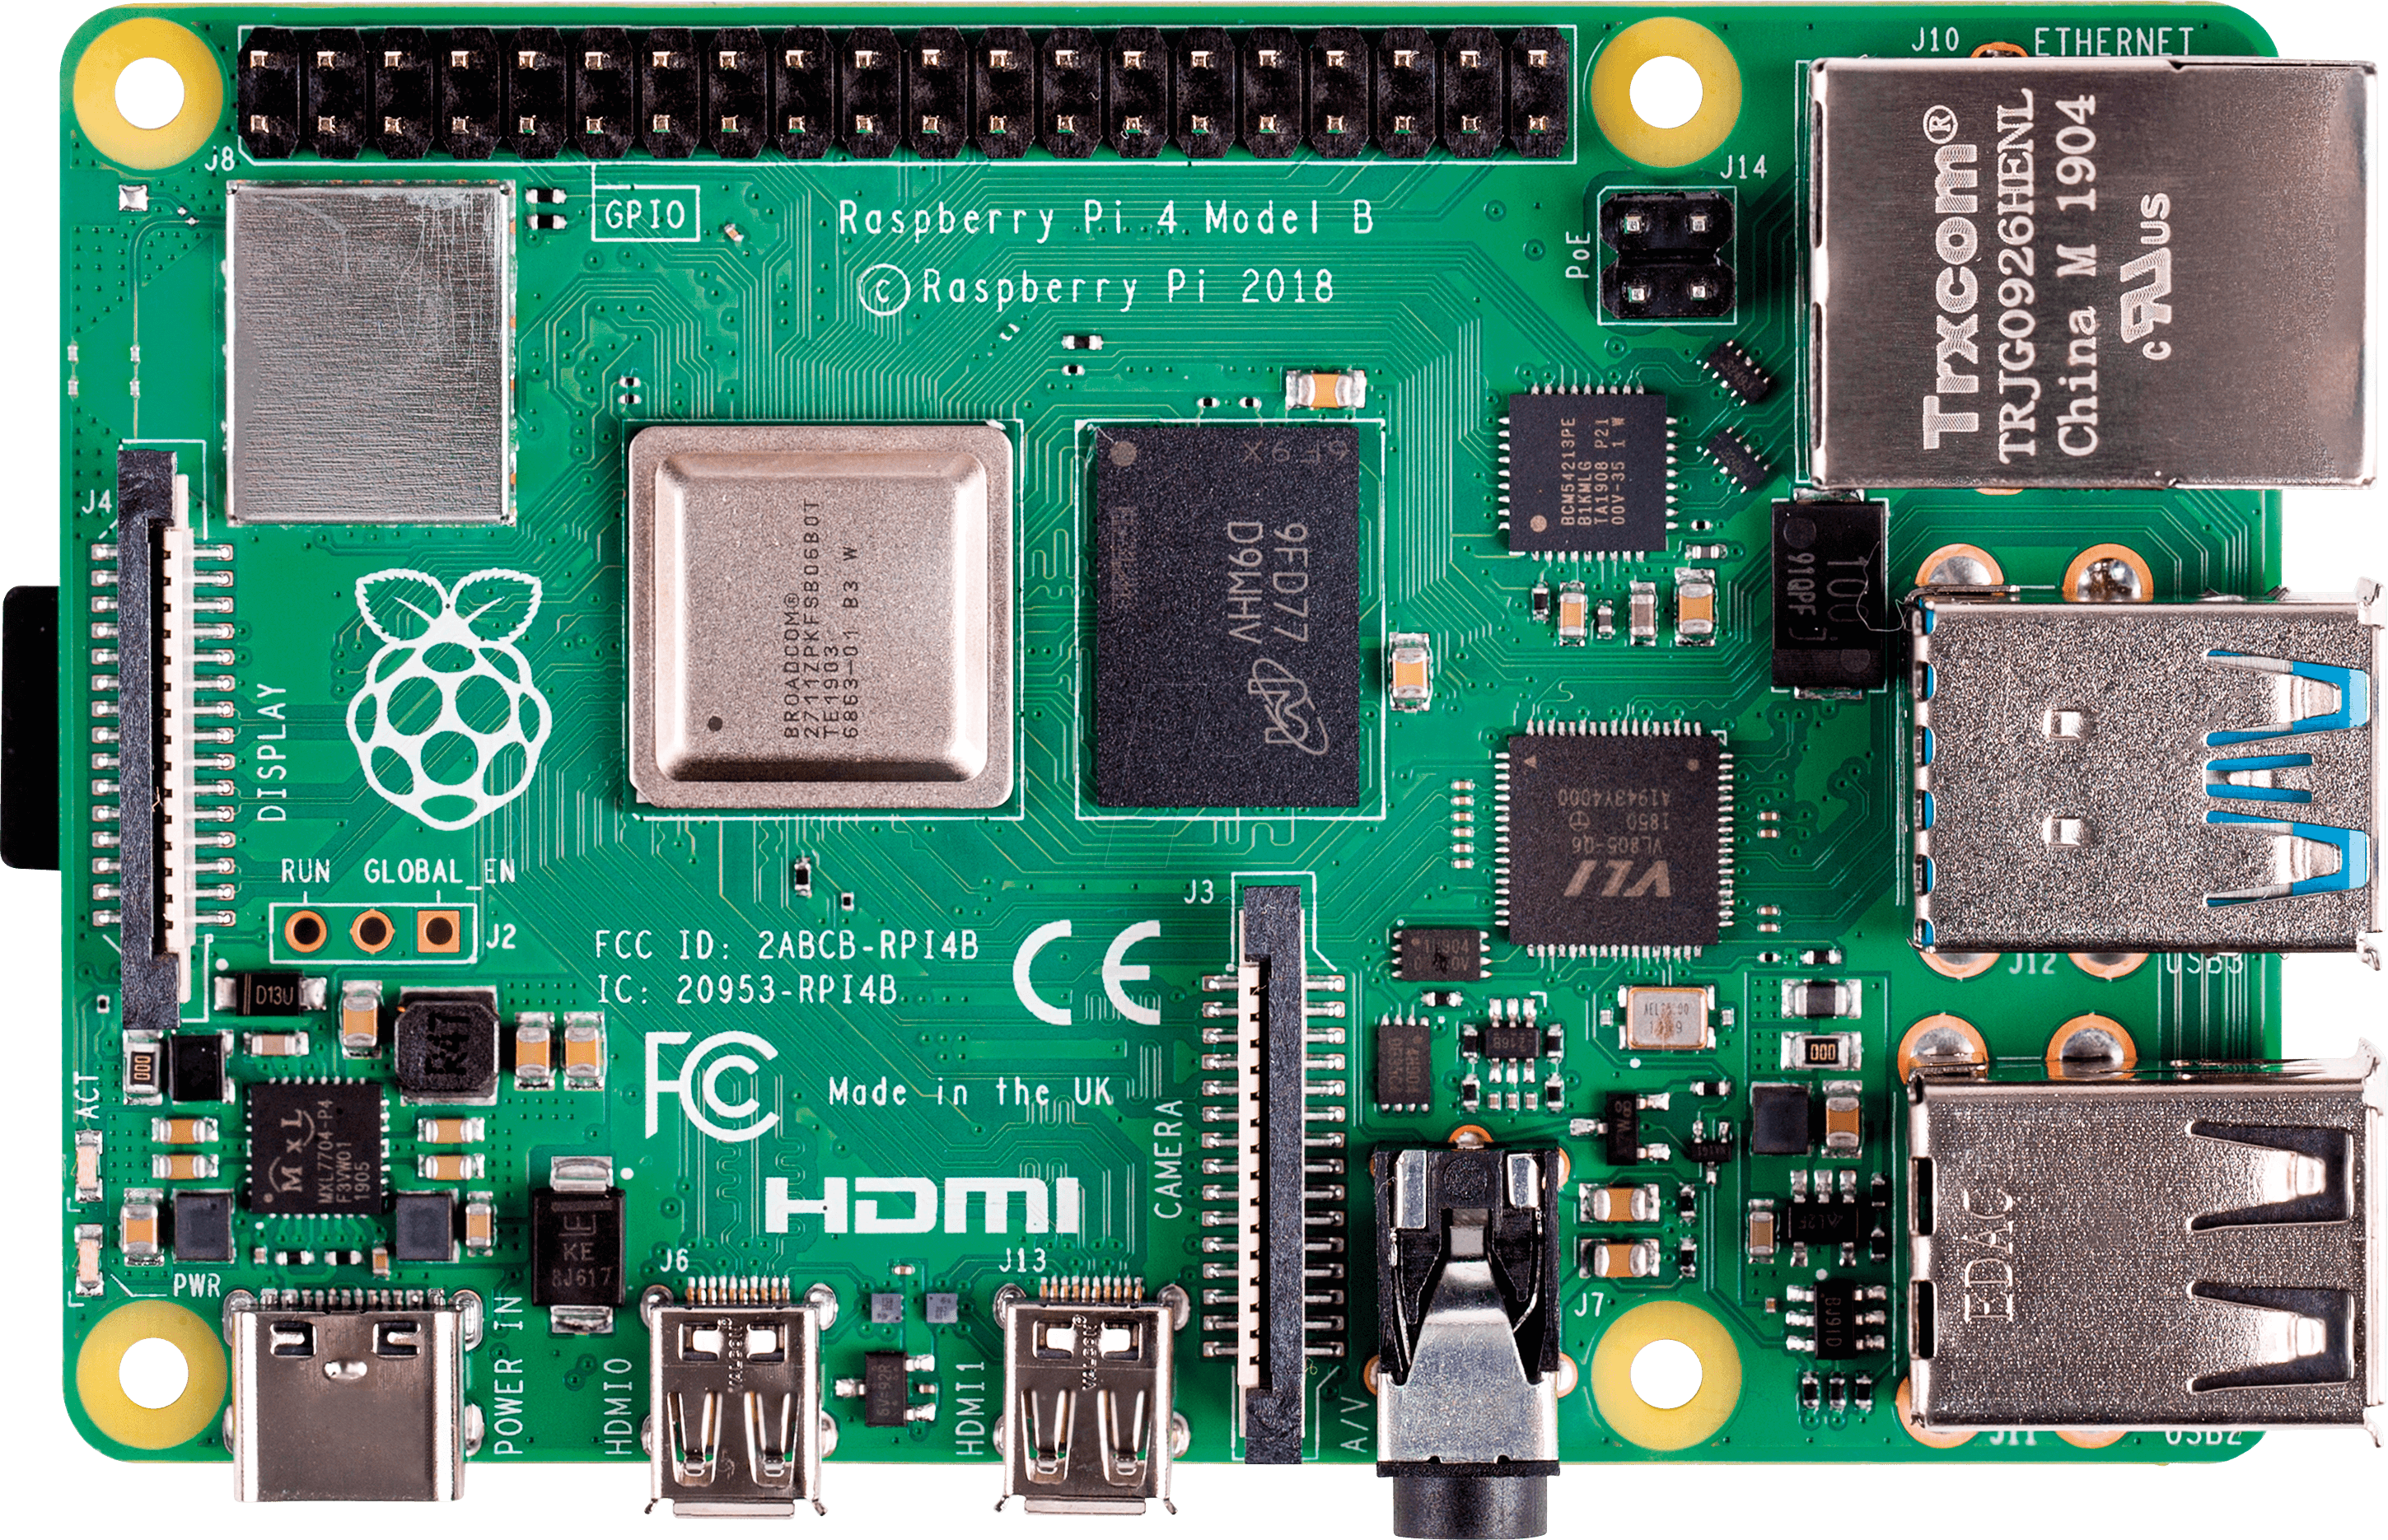
\includegraphics[width=\linewidth, angle=270]{pics/RPI4B.png}
    \end{minipage}\hfill
    \caption{Raspberry Pi 4 Model B and its specifications}\label{tab:rpi4_specs}
\end{table}



\vspace{2em}

\begin{table}[h]
    \begin{minipage}{0.6\textwidth}
        \centering
        \renewcommand{\arraystretch}{2.0}
        \setlength{\tabcolsep}{4.4pt}
        \footnotesize
        \begin{tabular}{|p{2.9cm}|p{6.4cm}|}
          \hline
          \rowcolor[gray]{0.8} 
          \textbf{Parameter} & \textbf{Value} \\
          \hline
          SoC & ESP-WROOM-32 module \\
          \hline
          Processor & Dual-core 32-bit processor with built-in 2.4 GHz Wi-Fi and Bluetooth \\
          \hline
          Memory & 4MByte flash memory \\
          \hline
          Operating Voltage & 2.2 to 3.6V \\
          \hline
          Breakout & In breadboard-friendly breakout \\
          \hline
          USB & USB micro B \\
          \hline
        \end{tabular}
    \end{minipage}
    \begin{minipage}{0.47\textwidth}
        \centering
        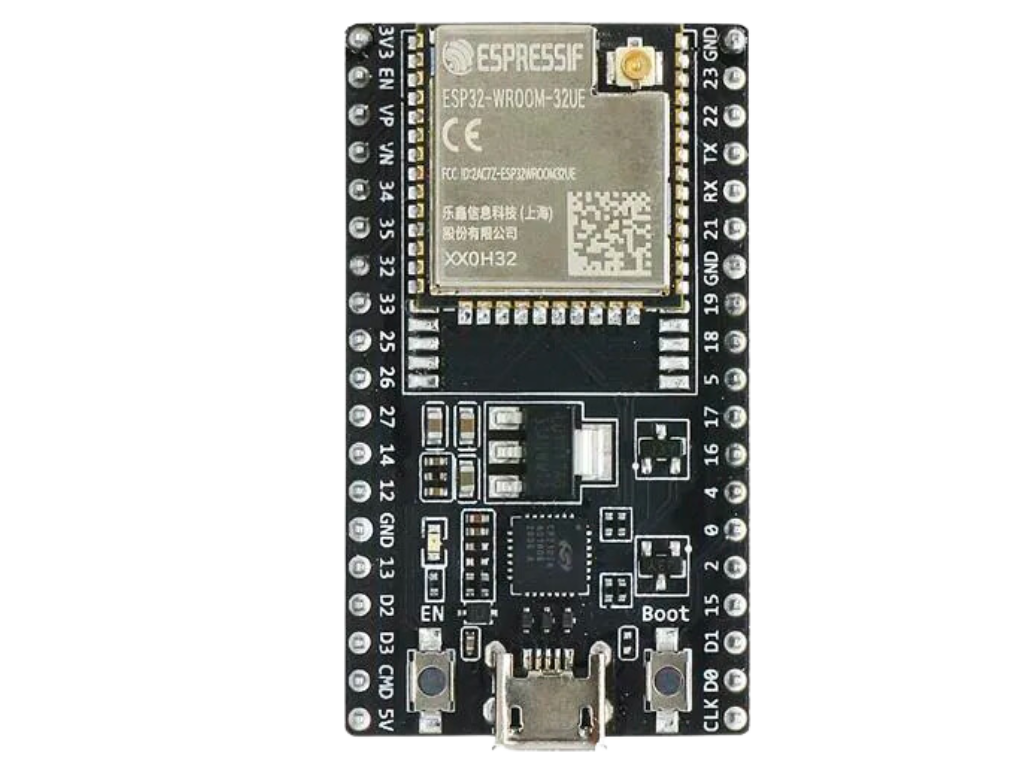
\includegraphics[width=\linewidth, angle=360]{pics/esp32.png}
    \end{minipage}\hfill
    \caption{NodeMCU ESP32 and its specifications}\label{tab:nodemcu}
\end{table}



\newpage


\subsubsection{Motor Controller}

\vspace{-0.6em}

Since the robot will be navigating in a hospital environment, electric motors will be used for this
application as they reduce noise level and CO$_2$ emissions. This also fulfills the ISO 23482-2:2019 which provides guidance
on new safety terms and requirements to enable close human-robot interaction. The motors will be controlled by an L298N motor driver. The
XH-M249 / XY-3606 steps down the voltage from battery 24V to 5V for the microcontrollers and other components.

\vspace{1em}


\begin{table}[h]
    \begin{minipage}{0.6\textwidth}
        \centering
        \renewcommand{\arraystretch}{2.0}
        \setlength{\tabcolsep}{4.4pt}
        \footnotesize
        \begin{tabular}{|p{4.5cm}|p{4.5cm}|}
          \hline
          \rowcolor[gray]{0.8} 
          \textbf{Parameter} & \textbf{Value} \\
          \hline
          Driver Chip &  Double H Bridge L298N \\
          \hline
          Motor Supply Voltage (max) & 46V \\
          \hline
          Motor Supply Current (max) & 2A \\
          \hline
          Logic Voltage & 5V \\
          \hline
          Driver Voltage & 5V -- 35V \\
          \hline
          Logic Current & 0 -- 36mA \\
          \hline
          Driver Current & 2A \\
          \hline
          Maximum Power & 25W \\
          \hline
        \end{tabular}
    \end{minipage}
    \begin{minipage}{0.36\textwidth}
        \centering
        \includegraphics[width=\linewidth, angle=360]{pics/l298n.png}
    \end{minipage}\hfill
    \caption{L298N Motor Driver and its specifications}\label{tab:l298n}
\end{table}

\vspace{-0.4em}


\begin{table}[h]
    \begin{minipage}{0.6\textwidth}
        \centering
        \renewcommand{\arraystretch}{2.0}
        \setlength{\tabcolsep}{4.4pt}
        \footnotesize
        \begin{tabular}{|p{4.0cm}|p{5.0cm}|}
          \hline
          \rowcolor[gray]{0.8} 
          \textbf{Parameter} & \textbf{Value} \\
          \hline
          Driver Chip &  XH-M249 / XY-3606 \\
          \hline
          Input Voltage & DC 9V -- 36V \\
          \hline
          Output Voltage & 5.2V / 5A / 25W \\
          \hline
          Output Voltage & $V_{out} = 5V$ DC ($V_{in} \geq V_{out} + 1.5V$) \\
          \hline
          Output capability & Input: 9 $\sim$ 24V  \newline Output: 5.2V / 6A / 30W \\
          
           & Input: 24 $\sim$ 32V \newline  Output: 5.2V / 5A / 25W \\
          
           & Input: 32 $\sim$ 36V \newline Output: 5.2V / 3.5A / 18W \\
          \hline
          Size & 63 * 27 * 10cm (L * W * H) \\
          \hline
        \end{tabular}
    \end{minipage}
    \begin{minipage}{0.36\textwidth}
        \centering
        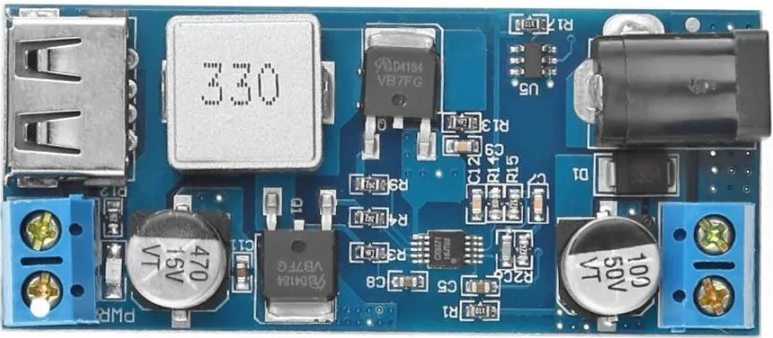
\includegraphics[width=\linewidth, angle=90]{pics/xr.png}
    \end{minipage}\hfill
    \caption{DC Step Down XH-M249 / XY-3606 and its specifications}\label{tab:l298n}
\end{table}




\newpage
\subsection{Software Implementation}

\subsubsection{Ecosystem}
This project uses a sophisticated software ecosystem to achieve autonomous navigation and medicine dispensing. The Robot Operating System 2 (ROS2) is the middleware, enabling seamless communication and integration between various software components. 

\vspace{0.4in}

\begin{figure}[H]
    \centering
    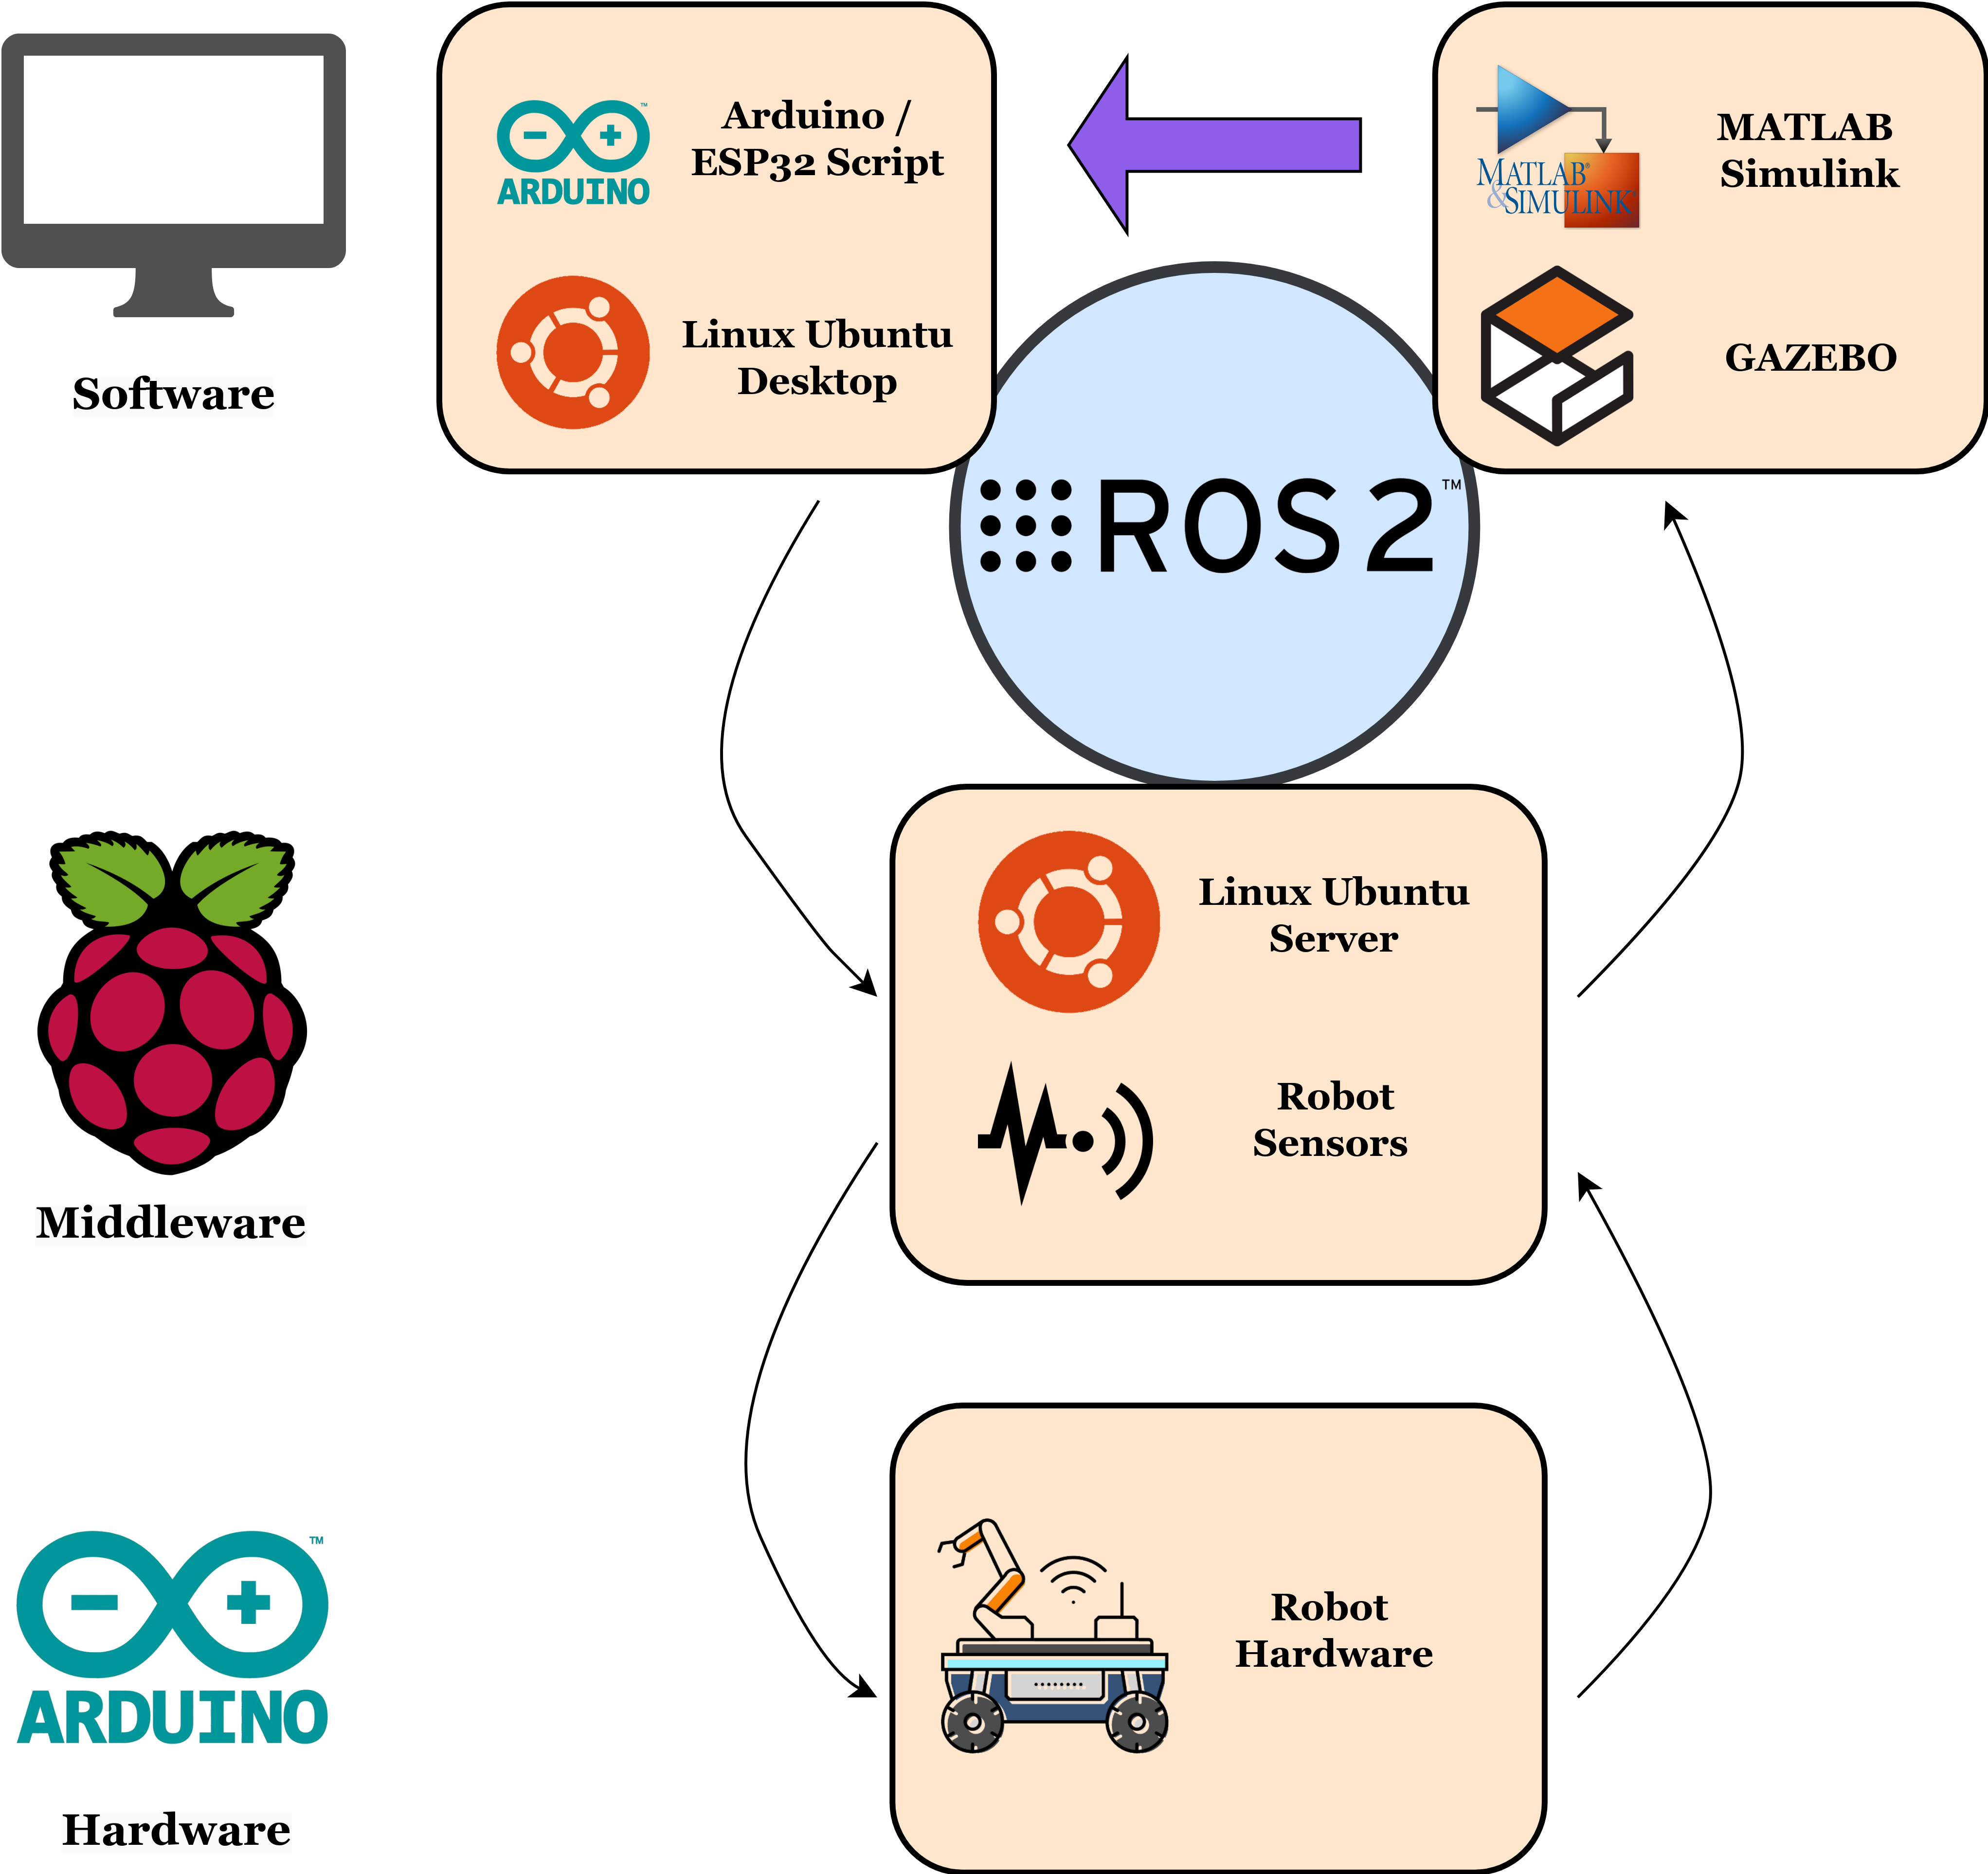
\includegraphics[width=6.2in]{pics/illustration.png}
    \caption{ROS2 Ecosystem}\label{ros2}
\end{figure} 

\vspace{0.4in}


\noindent A headless Raspberry Pi 4, running an Ubuntu server and ROS2 Humble Hawksbill, acts as the central processing unit. This configuration optimizes computational resources by eliminating the overhead of a graphical user interface. The Raspberry Pi communicates with an ESP32 microcontroller, which handles low-level control functions like motor control and sensor data acquisition.
ROS2's node architecture facilitates the integration of sensor data from the LiDAR, IMU sensor, encoder wheels, ultrasonic and Time of Flight sensors. This data is then processed and visualized using a combination of Gazebo and RViz2. These tools provide a view of the robot's environment and its interactions. MATLAB's Simscape and Simulink tools could also be integrated with ROS2 to offer an alternative visualization method and enable potential future utilization of MATLAB's extensive capabilities.
A vital aspect of this project is the development of a "digital twin." This digital twin will mirror the actions and movements of the physical robot in a simulated environment. This approach allows for real-time remote feedback and facilitates virtual simulations, enabling the testing and refinement of navigation algorithms without relying solely on physical trials. This not only accelerates the development process but also conserves resources and energy.





\subsubsection{User Interface} 
User interface is an important part of the robot system as the robot has to meet basic safety standards and also, it has
to interact easily with the operator. This interface will comprise of switches for user input mounted on the robot, as well as
a Graphical User Interface (GUI) on the workstation computer for remote monitoring and control. Subsequently, the ISO 15066:2016 standard defines safe ways in which 
humans can interact with robots. It mandates the necessity of including emergency stop mechanisms. As such, the signal shall be an emergency switch infront of the robot
which is very accessible. When pressed, the robot will halt and stop all movement operations. To interact with the robot's navigation 
and mapping system, most of the
operations can be achieved through a terminal-driven interface, but a graphical user interface (GUI) will be more
intuitive and user-friendly especially for non-technical users. There are several tools and external softwares
e.g Foxglove, that can be adapted to develop the user interface. However, building a custom GUI offers more control
and flexibility in terms of design and functionality. Qt is a cross-platform application framework used for developing
GUIs. Qt supports C++ and integrates well with ROS2, hence it is chosen for this project. 

\subsubsection{System Architecture}
The system architecture of the autonomous medicine dispensing robot, as shown in the Figure~\ref{system} below, comprises
a network of interconnected hardware and software components. The power system, driven by a 24V 22Ah LiPo battery, supplies
energy to the robot. A DC-DC buck converter (XH-M249) steps down this voltage to 12V and 5V to power various components, including the processing
units and sensors. The primary processing unit is a Raspberry Pi 4B 8GB. It communicates with an Arduino UNO 
via UART, delegating low-level control functions such as motor control and encoder data acquisition. An ESP32
is also integrated into the system, which connects wirelessly
with the Raspberry Pi.
The robot's sensing system includes a 2D RP-LIDAR A1 M8 for 360-degree environmental scanning, three HCR-S04 ultrasonic sensors
for perimeter obstacle detection, a VL53L0X V2 Time-of-Flight sensor for precise frontal distance measurement, an MPU9250 IMU 
for motion sensing, and an NTC temperature sensor for thermal monitoring. Actuation is achieved through an L298N motor driver,
which controls two motors equipped with encoders for precise movement. Cooling fan ensure the electronics maintain a safe operating temperature.
Communication within the system is facilitated through various protocols, including UART for short-range connections, SSH
for secure remote access to the Raspberry Pi, and Wi-Fi (TCP/IP) for wireless
communication with the GUI workstation. A USB hub could expand the Raspberry Pi's connectivity options, especially when debugging,
but it is unnecessary when the robot operates. The user interface comprises a keypad, extra switches on the robot itself, and
a GUI workstation for more complex user interactions and monitoring. 

\vspace{0.15in}

\begin{figure}[H]
    \centering
    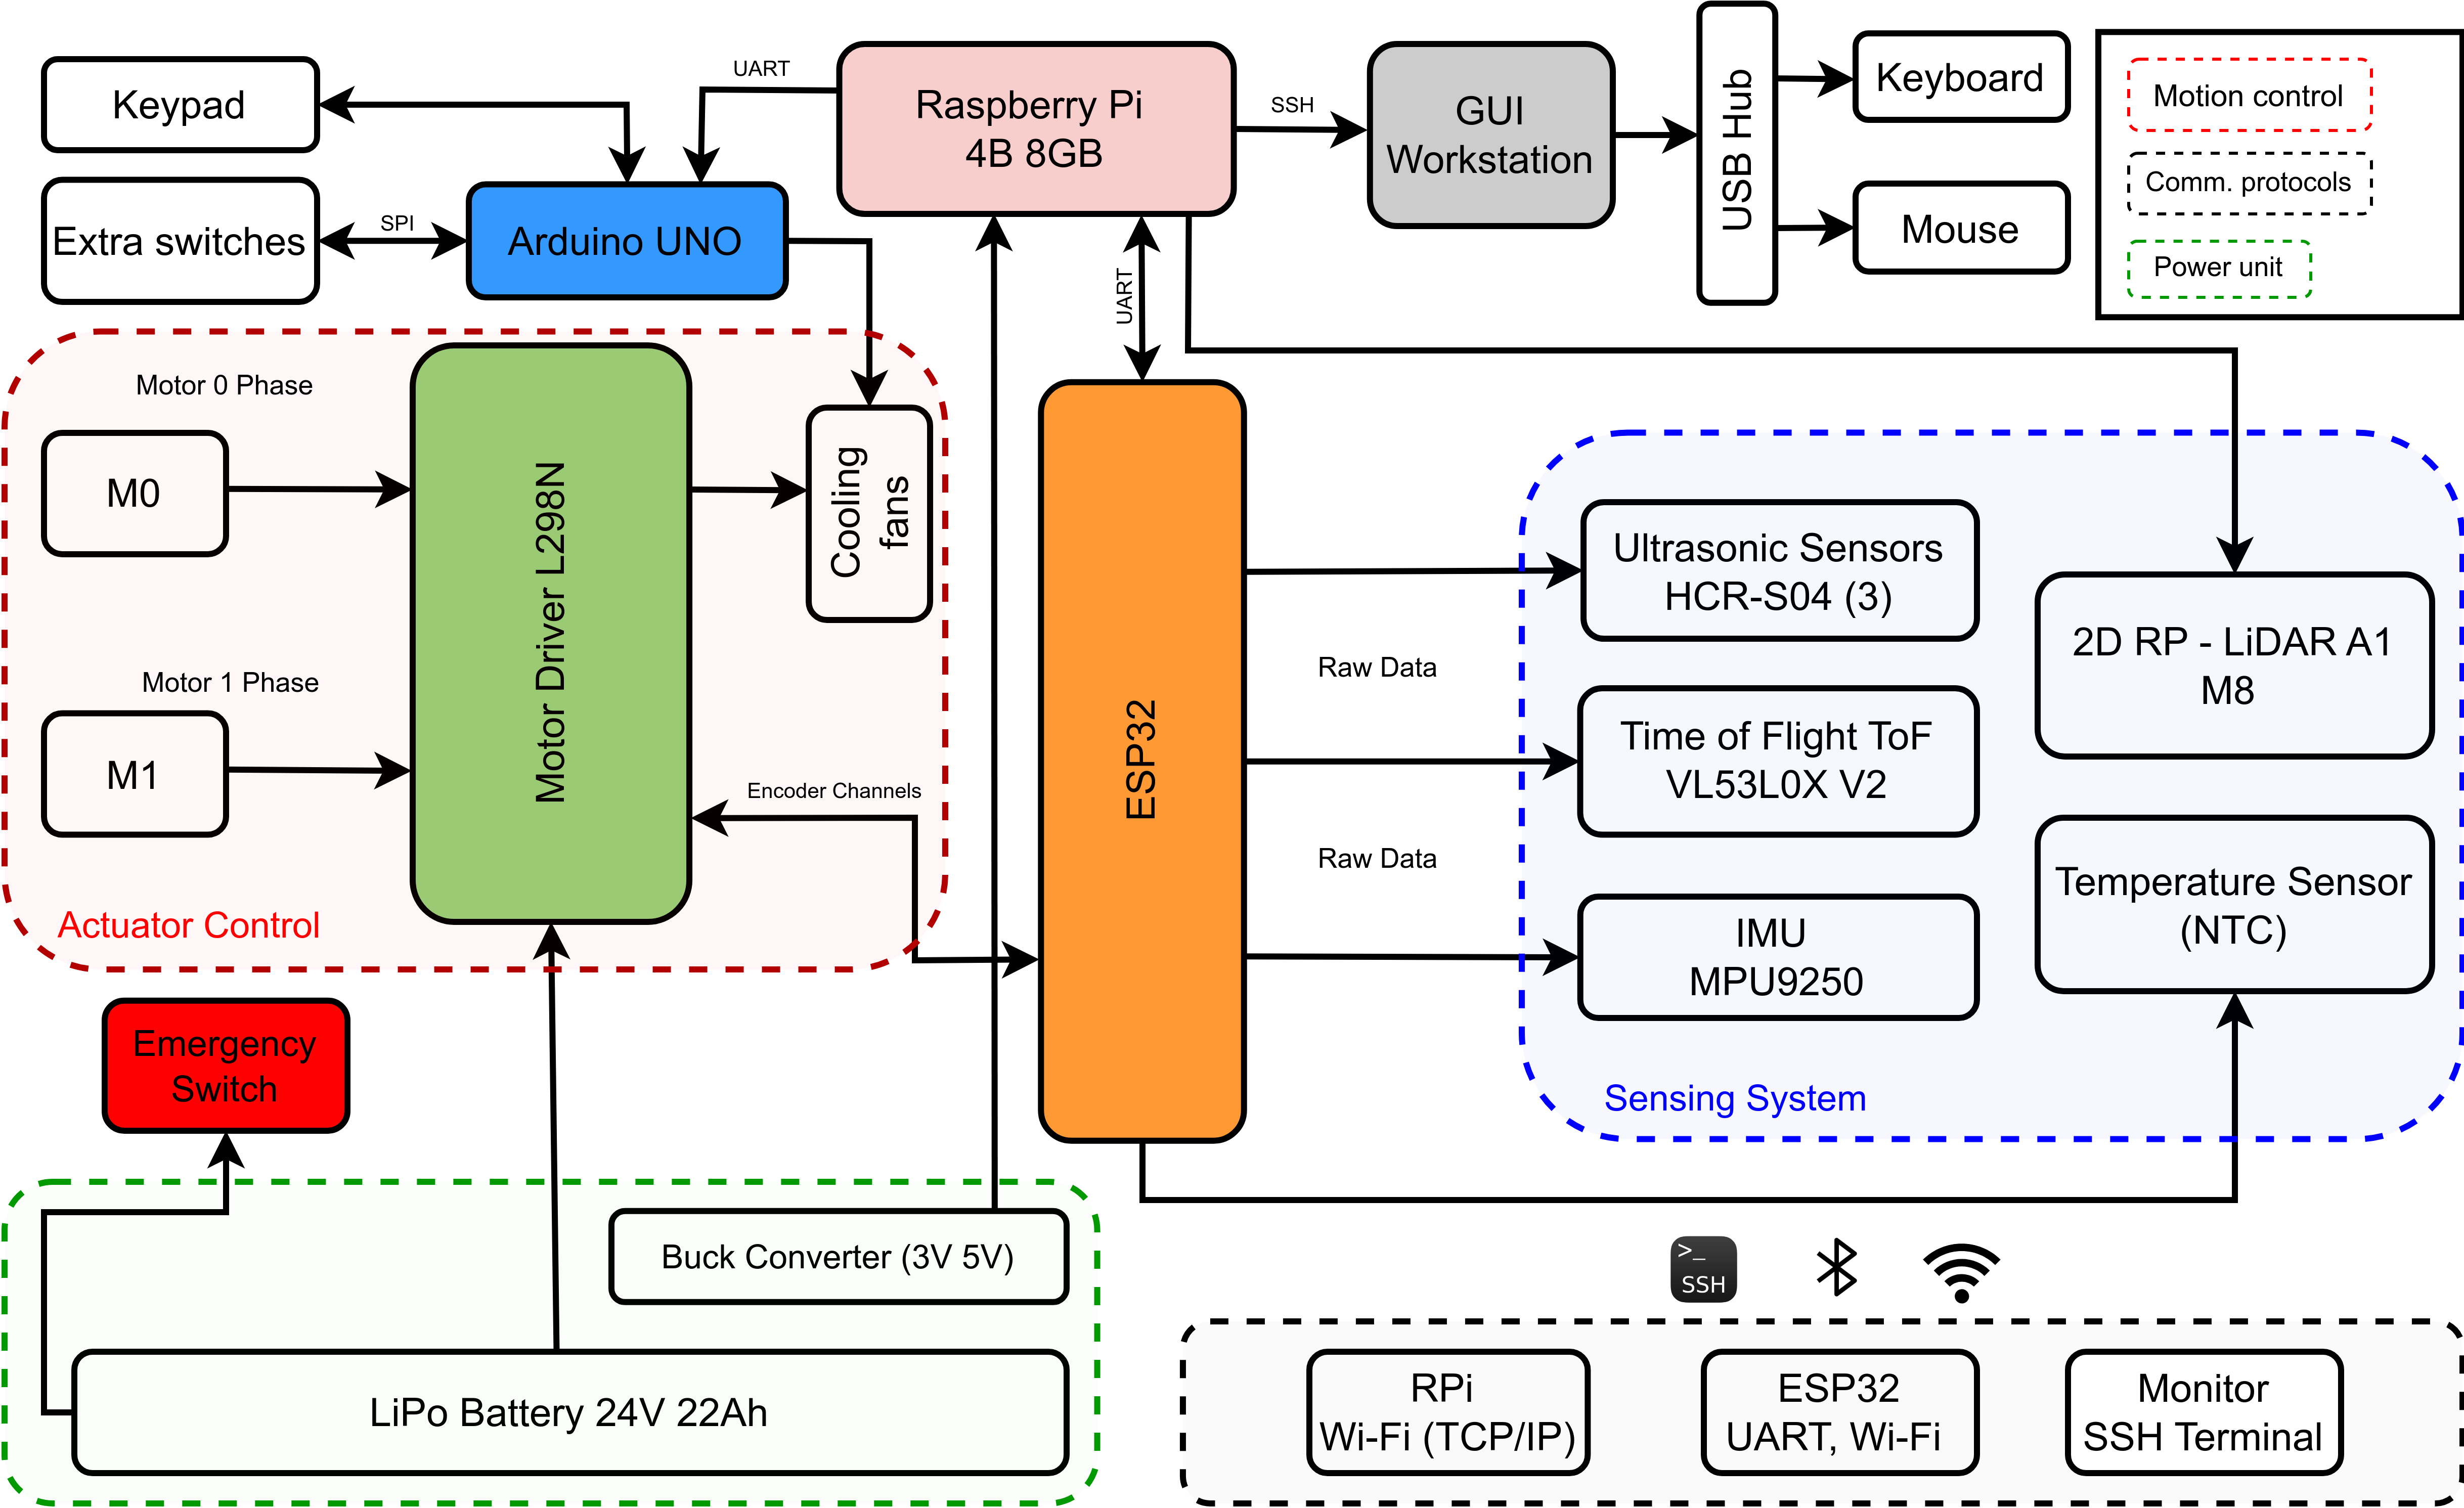
\includegraphics[width=6.1in]{pics/Hardware_Architecture3.png}
    \caption{System Architecture Overview}\label{system}
\end{figure} 



%\newpage


%\newpage


% GanttHeader setups some parameters for the rest of the diagram
% #1 Width of the diagram
% #2 Width of the space reserved for task numbers
% #3 Width of the space reserved for task names
% #4 Number of months in the diagram
% #5 Start year
% In addition to these parameters, the layout of the diagram is influenced
% by keys defined below, such as y, which changes the vertical scale
\def\GanttHeader#1#2#3#4#5{%
 \pgfmathparse{(#1-#2-#3)/#4}
 \tikzset{y=8mm, 
     task number/.style={
         left, 
         font=\scriptsize\bfseries, 
         minimum width=1.2ex, 
         align=right,
         text width=1.4ex
     },
     task description/.style={text width=#3, right, draw=none,
           font=\scriptsize\sffamily, xshift=#2,
           minimum height=2em, text justified},
     gantt bar/.style={draw=black, fill=blue!30},
     help lines/.style={draw=black!30, dashed},
     x=\pgfmathresult pt
     }
  \def\totalmonths{#4}
  % Separate header text that's aligned with "Weeks"
  \node[anchor=west, xshift=#2] at (0,0.4) {\textbf{\small Task Description}};
  % Original column starting point (without moving up)
  \node (Header) [task description] at (0,0) {};
  \begin{scope}[shift=($(Header.south east)$)]
    \node[above=0.58cm] at (#4/2,0) {\textbf{\small Weeks}};
    \foreach \x in {1,...,#4}
      \node[above] at (\x,0.01) {\pgfmathparse{int(\x+#5)}\footnotesize\pgfmathresult};
 \end{scope}
}

% This macro adds a task to the diagram
% #1 Number of the task
% #2 Task's name
% #3 Starting date of the task (month's number, can be non-integer)
% #4 Task's duration in months (can be non-integer)
% #5 Deadline flag (0 or 1)
\def\Task#1#2#3#4#5{%
\node[task number] at ($(Header.west) + (-0.02ex, -#1+0.049)$) {#1};
\node[task description] at (0,-#1) {#2};
\begin{scope}[shift=($(Header.south east)$)]
  \draw (0,-#1) rectangle +(\totalmonths, 1);
  \foreach \x in {1,...,\totalmonths}
    \draw[help lines] (\x,-#1) -- +(0,1);
  \ifnum#5=1 % If it has a deadline
    \filldraw[gantt bar] ($(#3, -#1+0.2)$) rectangle +(#4-1,0.6);
    \filldraw[draw=black, fill=red!30] ($(#3+#4-1, -#1+0.2)$) rectangle +(1,0.6);
  \else % If it's an ongoing task
    \filldraw[gantt bar] ($(#3, -#1+0.2)$) rectangle +(#4,0.6);
  \fi
\end{scope}
}

% Example



\section{Project Planning and Management}


\subsection{Plan of Action}
This project will be conducted primarily within Swinburne University of Technology, Sarawak Campus. The project demonstration, 
hardware assembly, and testing will be conducted at the university's facilities, including the engineering labs. Necessary 
components will be sourced through online vendors (OTS), and others will be supplemented by existing components available in the university's
inventory. Throughout the project, comprehensive documentation, a detailed final report, and a presentation 
demonstrating the project's outcomes will be conducted for FYRP1 and FYRP2. Weekly meetings will be held with the supervisors 
to discuss progress challenges and receive feedback. A detailed logbook and meeting minutes of all the activities will 
be submitted by the end of the semester. As for the project timeline, Final Year Research Project 1 (FYRP1) will mainly cover the project's research part. The idea will also
be designed using CAD software, and simulation will be conducted for testing and proof of concept. The final project implementation
will be done in the Final Year Research Project 2 (FYRP2). The Gantt chart for FYRP1 and FYRP2 is shown in Figure \ref{fig:gantt-chart} and \ref{fig:gantt-chart2} respectively.


\subsection{Risk Management}
Some potential risks include a delay in shipment of the project components after ordering, especially the LiDAR sensor, which
is harder to find from local vendors. In such a case, alternative suppliers will be considered, and other sensors 
will be used for initial development. Delaying and procrastination also pose a risk to the project, which will be mitigated by regular
self-monitoring. Progress evaluations from the supervisor will be conducted to ensure adherence to the schedule. Furthermore,  
technical challenges could arise during the project implementation, such as unexpected hardware failure or difficulty in software integration with 
the sensors and the ROS2 framework. An iterative approach will be adopted, and a comprehensive testing and debugging strategy will 
be employed to resolve any technical issues promptly. Finally, the budget allocated for the project might need to be increased, hindering the project's progress. Regular communication with the supervisors will be prioritized to ensure the budget is utilized effectively.


\newpage

\subsection{Project Timeline (Gantt Chart)}


\vspace{-0.1in}


\begin{figure}[ht]
  \centering
  \begin{tikzpicture}
    \GanttHeader{.98\textwidth}{2.1ex}{4.0cm}{14}{0} % 14 weeks in sem 
    \Task{1}{Project Registration }{0}{2}{1}
    \Task{2}{Research plan development}{1}{2}{0} % Task 2
    \Task{3}{Literature review}{2}{3}{0} % Task 3
    \Task{4}{Mid semester presentation}{3}{3}{1} % Task 4
    \Task{5}{Research plan}{3}{5}{1} % Task 5
    \Task{6}{Preliminary testing (simulation)}{6}{5}{0} % Task 6
    \Task{7}{Proof of concept (simulation)}{8}{4}{0} % Task 7
    \Task{8}{Poster Presentation}{9}{3}{1} % Task 8
    \Task{9}{Workbook}{0}{13}{1} % Task 9
    \Task{10}{Progress Report}{10}{4}{1} % Task 10 
    
    % Add legend/key
    \node[below=1.0cm of current bounding box.south west, anchor=west] {
      \begin{tikzpicture}[baseline=0]
        % Legend for ongoing task
        \draw[fill=blue!30] (0,0) rectangle (0.5,0.3);
        \node[right, font=\footnotesize] at (0.5,0.15) {Ongoing task};
        
        % Legend for deadline
        \draw[fill=red!30] (3.3,0) rectangle (3.8,0.3);
        \node[right, font=\footnotesize] at (3.8,0.15) {Deadline};
      \end{tikzpicture}
    };
  \end{tikzpicture}
  \caption{Final Year Project 1 Timeline Gantt Chart.}\label{fig:gantt-chart}
  \end{figure}
  
  

\vspace{0.2in}

% Example

\begin{figure}[H]
\centering
\begin{tikzpicture}
  \GanttHeader{.98\textwidth}{2.1ex}{4.0cm}{14}{0} % 14 weeks in sem 
  \Task{1}{Order hardware parts}{0}{2}{0}
  \Task{2}{Hardware assembly/integration}{1}{2}{0} % Task 2
  \Task{3}{Sensor integration and testing}{2}{3}{0} % Task 3
  \Task{4}{Implement navigation algorithm}{3}{3}{0} % Task 4
  \Task{5}{User interface integration}{3}{5}{0} % Task 5
  \Task{6}{Final choice (algorithms)}{6}{5}{0} % Task 6
  \Task{7}{Optimizing software / iteration}{8}{4}{0} % Task 7
  \Task{8}{Validation and perfomance}{9}{3}{0} % Task 8
  \Task{9}{Workbook}{9}{4}{1} % Task 9
  \Task{10}{Final Report}{10}{4}{1} % Task 10 
  
  % Add legend/key
  \node[below=1.0cm of current bounding box.south west, anchor=west] {
    \begin{tikzpicture}[baseline=0]
      % Legend for ongoing task
      \draw[fill=blue!30] (0,0) rectangle (0.5,0.3);
      \node[right, font=\footnotesize] at (0.5,0.15) {Ongoing task};
      
      % Legend for deadline
      \draw[fill=red!30] (3.3,0) rectangle (3.8,0.3);
      \node[right, font=\footnotesize] at (3.8,0.15) {Deadline};
    \end{tikzpicture}
  };
\end{tikzpicture}
\caption{Final Year Project 2 Timeline Gantt Chart.}
\label{fig:gantt-chart2}
\end{figure}











\newpage
\subsection{Bill of Materials}
The bill of materials is categorised into three different types,
(a) the mechanical stucture unit, (b) off-the-shelf (OTS) components are the electronics, control devices, 
sensors, and power sources, (c) the manufacturing tools. The total cost of the project is estimated to be RM888.20. 

\vspace{0.4in}

\begin{table}[h]
    \centering
    \scriptsize % Reduces the text size significantly
    \renewcommand{\arraystretch}{1.4} % Adjust the row height

    % Set the total table width and define individual column widths
    \begin{tabular}{>{\raggedright\arraybackslash}p{0.3cm} >{\raggedright\arraybackslash}p{5.5cm} >{\raggedleft\arraybackslash}p{1.0cm} >{\raggedleft\arraybackslash}p{1.5cm} >{\raggedleft\arraybackslash}p{1.5cm} >{\raggedright\arraybackslash}p{2.2318cm}}
        \toprule
        \textbf{No.} & \textbf{Description} & \textbf{Qty} & \textbf{Unit Cost} & \textbf{Total cost} & \textbf{Source of Material} \\
        \midrule
        \multicolumn{6}{l}{\textbf{Mechanical Structure Unit}} \\
        P1&Profile 20x20L I-type 400cm  &400&0.23   & 92.00 &\href{https://shopee.com.my/-Customize-Length-Aluminium-Profile-2020-2040-3030-4040-For-European-Standard-i.118650399.5905411154?sp_atk=386a0d30-c468-47ce-b8a4-6ad3d9f9ddbd&xptdk=386a0d30-c468-47ce-b8a4-6ad3d9f9ddbd}{Shopee}  \\
        P2&Pivot / Knuckle Joint for 2020 &4&16.50& 66.00  &  \href{https://shopee.com.my/Pivot-Joint-Knuckle-Joint-Swivel-Joint-for-2020-3030-4040-4545-Aluminium-Profile-i.197714890.8716364314?sp_atk=363c4a5d-dac2-4810-b09c-7a37cb79c45d&xptdk=363c4a5d-dac2-4810-b09c-7a37cb79c45d}{Shopee}\\
        P3&L Corner Bracket Gusset Element (2020)& 18&2.00  & 36.00 & \href{https://shopee.com.my/L-Corner-Bracket-Gusset-Element-L-Bracket-Connector-1720-2028-3030-4040-3060-4080-Aluminium-Profile-i.118650399.7404726140?sp_atk=9cb10872-5679-4217-8a7b-700cf159c424&xptdk=9cb10872-5679-4217-8a7b-700cf159c424}{Shopee}  \\ 
        P4&L Bracket (Stainless Steel)& 12  &1.20  & 14.40 & \href{https://shopee.com.my/L-Bracket-Solid-Angle-Bracket-Stainless-Steel-Thick-High-Quality-i.243397959.7565902322?sp_atk=bfd4a0f4-841b-4fa1-a8e5-5c514175fb8c&xptdk=bfd4a0f4-841b-4fa1-a8e5-5c514175fb8c}{Shopee} \\ 
        P5&Axial fan &1&-&-&-  \\
        P6&Screw / bolt &100&0.30& 30.00 &-  \\
        P7&Nuts &100& 0.15&15.00 &-  \\
        P8&Drive wheels (Pneumatic) \diameter120---150mm &2&-&-&-  \\
        P9&Swivel caster \diameter90-110mm & 1 & 14.70 &   14.70 & \href{https://shopee.com.my/MEDIUM-DUTY-3-INCH-Caster-PU-Wheel-Orange-Rigid-Swivel-With-Brake-360-Degree-Industrial-Quiet-Replacement-Wheel-Trolley-i.1530870.25363469103?sp_atk=fcfd4f24-1d19-45ba-9076-e04b23158c9e&xptdk=fcfd4f24-1d19-45ba-9076-e04b23158c9e}{Shopee} \\
        P10&Plywood (l by w)&-& 40.00 &   40.00 &-  \\
        \midrule
        \multicolumn{6}{l}{\textbf{OTS electronics, sensors and control devices}} \\
        P11&Raspberry Pi4 8 GB  &1& 389.0 &-& \href{https://my.cytron.io/c-raspberry-pi-main-board}{Cytron} \\
        P12&NODEMCU ESP32 & 1 &29.00&-& \href{https://my.cytron.io/p-nodemcu-esp32?r=1}{Cytron} \\
        P13&Arduino UNO R3 ATMEGA328P& 1 &44.90&-& \href{https://shopee.com.my/%F0%9F%94%A5DIP-UNO-R3%F0%9F%94%A5Rev3-V3-Atmel-ATMEGA328P-Compatible-Board-Plug-and-Play-(No-need-download-extra-Arduino-USB-driver)-i.33091591.466533399?sp_atk=e3b3d732-4076-4741-9f4e-09b6b5c0a914&xptdk=e3b3d732-4076-4741-9f4e-09b6b5c0a914}{Shopee}\\
        P14&8GB MicroSD & 1 & 9.99&-& \href{https://shorturl.at/gBoSd}{Shopee} \\
        \begin{comment}
        &3.5'' TFT LCD (ILI9481-R61581, CTE32HR)& 1 & 65.00 & 65.00 & \href{https://shopee.com.my/3.5-Arduino-TFT-LCD-Module-(Colour-Screen)-i.40459773.6011888764?sp_atk=5d9e5d6e-564c-4295-88a1-3b68c3cec2c3&xptdk=5d9e5d6e-564c-4295-88a1-3b68c3cec2c3}{Shopee} \\
        &4x4 Matrix Keypad& 1 & 12.50 & 12.50 & \href{https://shopee.com.my/Keypad-Matrix-Black-4X4-4X3-Keyboard-Button-Telephone-4*4-4*3-Style-16-12-Key-Compatible-with-Arduino-i.608059940.15946050312?sp_atk=07d7390d-4f01-4074-8a62-9ae8ae1a0be5&xptdk=07d7390d-4f01-4074-8a62-9ae8ae1a0be5}{Shopee} \\
        \end{comment}
        P15&Time of Flight VL53L0X V2  & 1 & 15.20 & 15.20  & \href{https://shopee.com.my/VL53L0X-V2-Time-of-Flight-Distance-Sensor-i.6674515.1944349963}{Shopee} \\
        P16&RP LiDAR A1 M8 (2D)&1 & 340.00& 340.00& \href{https://trade.taobao.com/trade/detail/tradeSnap.htm?spm=a220l.16.0.0.216c25a5QZgyy0&tradeID=2238905640812998885}{Taobao}\\
        P17&IMU (MPU-9250) & 1 & 39.90 & 39.90& \href{https://shopee.com.my/MPU9250-MPU-9250-9-DOF-IMU-Module-Accelerometer-Gyroscope-Magnetometer-Balancing-Sensor-for-Arduino-i.33091591.678613373?sp_atk=d19e30a6-3796-46fe-b156-b40e4909d709&xptdk=d19e30a6-3796-46fe-b156-b40e4909d709}{Shopee} \\
        P18&Ultrasonic sensors (HCR-S04)& 3 &-&-&-  \\
        P19&22.2V LiPo battery 11AH & 2& 84.90& 169.80 & \href{https://shopee.com.my/7.4V-2S-11.1V-3S-25C-30C-1100mah-2200mah-5S-6000mah-22.2V-6S-Lipo-Li-po-Rechargeable-RC-Tamiya-Racing-Car-Drone-Battery-i.33091591.508615851?sp_atk=ad6d1510-cb5d-41f9-aada-10fd3eb6b045&xptdk=ad6d1510-cb5d-41f9-aada-10fd3eb6b045}{Shopee} \\
        P20&Mini Rocker Switch ON/OFF & 3 & 1.80 & 5.40 & \href{https://shopee.com.my/Mini-Rocker-Switch-ON-OFF-KCD11-6x6-12x12-14x9mm-Tact-Slide-Switch-DIP-SMD-Tactile-Self-Locking-Push-Button-Momentary-i.70429211.11217735748?sp_atk=74eb2c91-1add-4b4d-bee7-c6346d9eb101&xptdk=74eb2c91-1add-4b4d-bee7-c6346d9eb101}{Shopee} \\
        P21&Emergency Push Button &1& 9.80&9.80 &\href{https://shopee.com.my/LAY37-Emergency-Push-Stop-Red-Button-c-w-Casing-Box-1NO-1NC-i.35009139.11572334265?sp_atk=519450fc-bad1-41cb-9f9b-c65cac283322&xptdk=519450fc-bad1-41cb-9f9b-c65cac283322}{Shopee} \\
        P22&Buck Converter (XH-M249)&1 &$-$&$-$&\href{https://shopee.com.my/DC-Step-Down-(Fixed-5V)-XH-M249-XY-3606-5A.max-Buck-Converter-5V-9V-12V-24V-i.126211897.16930276280}{Shopee} \\
        P23&Motors (with encoders) & 2 &-&-&-  \\
        P24&Motor Driver L298N & 1 &-&-&- \\
        P25&SIRIM Cables 1.5mm Copper&-&-&-&-  \\
        P26&M2M M2F M2M F2F GPIO wires &-&-&-&-  \\
        \midrule
        \multicolumn{6}{l}{\textbf{Manufacturing Tools}} \\
        P27&Terminals &-&-&-&-  \\
        P28&Soldering station &-&-&-&  \\
        P29&Multimeters &-&-&-&-  \\
        P30&Breadboards &-&-&-&-  \\
        P31&Screws &-&-&-&-  \\
        P32&Fasteners &-&-&-&-  \\
        \midrule
        \rowcolor{red!10} & \textcolor{red}{\textbf{\small TOTAL}}  & & & \raggedleft{\textcolor{red}{888.20}} & \\
        \bottomrule
    \end{tabular}
    \caption{Bill of Materials (BOM) for the autonomous medical robot}\label{tab:bom}
\end{table}





%\newpage






\newpage


%\newpage


\begin{table}[h]
    \centering
    \begin{tabular}{|c|c|c|}
    \hline
    \textbf{Area} & \textbf{Coordinates (x, y)} & \textbf{Orientation} \\
    \hline
    2514 & (429, 361) & 83.4827 \\
    1817 & (432, 288) & -4.4490 \\
    1191 & (441, 194) & -5.5570 \\
    \hline
    \end{tabular}
    \caption{Object Coordinates}
    \label{tab:object_properties}
\end{table}
    





%\newpage
\section{Module Interfacing and Robot Arm Programming}
Hye The d fmdodule for interfacing and programming the robot arm in \texttt{ABB RobotStudio®} involved establishing bidirectional communication between \texttt{MATLAB} and the robot controller to enable efficient pick and place operations. The \texttt{RAPID} programming language was employed to develop the robot program, allowing it to receive real-time instructions from \texttt{MATLAB} based on object properties identified through image processing.

\subsection{Communication Setup:}
Interfacing of \texttt{MATLAB} and \texttt{RobotStudio} in Client/Server Communication: \\ 
\noindent \textbf{\texttt{MATLAB} (Client):} \\
\texttt{MATLAB} is responsible for performing image processing and identifying the properties of the objects to be manipulated. It sends the coordinates, rotation angles, and properties of these objects to the robot controller over a socket connection. \texttt{MATLAB} also receives acknowledgment messages from the robot controller to confirm that the data has been received and processed correctly. \\
\noindent \textbf{\texttt{ABB RobotStudio} (Server):} \\
The robot controller, programmed in \texttt{RAPID} within \texttt{RobotStudio}, acts as the server in this setup. It listens for incoming connections from \texttt{MATLAB} and receives data strings representing the objects' properties.

\begin{figure}[H]
    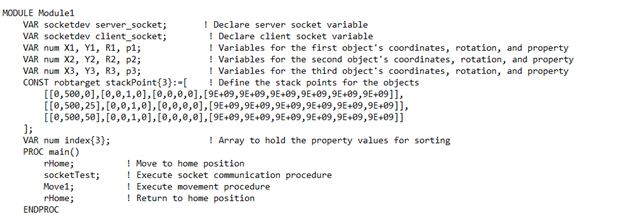
\includegraphics[width=7.4in ]{pics/abbstud.png}
    \label{abrrr}
\end{figure}

\textbf{Main Procedure (\texttt{main()}):} \\
The main procedure \texttt{main()} first calls \texttt{rHome()} to move the robot arm to the home position. It then executes the \texttt{socketTest()} procedure to establish the communication and receive data from \texttt{MATLAB}. Once the data is received, it is stored in an array (\texttt{index}) for sorting based on the properties of the objects.

The robot program begins with the declaration of server and client socket variables (\texttt{server\_socket} and \texttt{ client\_socket}). These sockets are essential for establishing the communication link between \texttt{MATLAB} and the \texttt{ABB} robot system. \texttt{MATLAB} acts as the client, sending data to the robot controller, which operates as the server, receiving and processing the data to execute the desired pick and place operations.

The \texttt{socketTest()} procedure handles the entire socket communication process. Initially, the server socket is created and configured with the \texttt{SocketCreate} and \texttt{SocketBind} commands. The server listens for incoming connections using \texttt{SocketListen}, and once a connection is accepted, \texttt{SocketAccept} establishes the communication link between the server and the client socket.


MATLAB sends data strings, which are received by the robot system using the SocketReceive function. These strings represent coordinates and properties of objects that need to be manipulated. The received data is converted from string format to numerical values using the StrToVal function and stored in predefined variables (X1, Y1, R1, p1) for each bar. After receiving and converting the data, the robot sends back acknowledgment messages to MATLAB using the SocketSend function.

\begin{center}
pickTargets{1}.trans := [X1, Y1, 0]; pickTargets{1}.rot := OrientZYX(R1, 0, 180); \\
pickTargets{2}.trans := [X2, Y2, 0]; pickTargets{2}.rot := OrientZYX(R2, 0, 180); \\
pickTargets{3}.trans := [X3, Y3, 0]; pickTargets{3}.rot := OrientZYX(R3, 0, 180); 
\end{center}



This part initializes the pickTargets array with the coordinates and rotations of the three bars. Each pickTargets element corresponds to a bar, with its position (trans) and orientation (rot) defined based on the received X, Y, and R values.

\begin{figure}[H]
    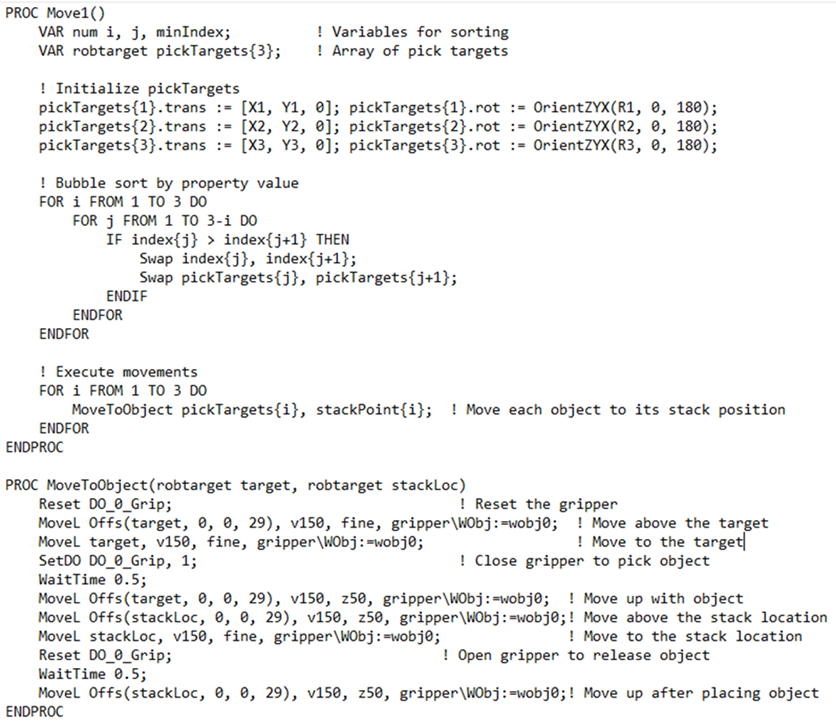
\includegraphics[width=5.5in ]{pics/PICKtARG.png}
    \label{PICK}
\end{figure}

\subsection{Movement and Sorting:}
In the \texttt{Move1} procedure, a bubble sort algorithm sorts the objects based on their properties. The sorted coordinates are then used to move the robot to each object's position. The \texttt{MoveToObject} procedure performs detailed pick and place actions, including moving to the object's location, gripping it, and placing it at the specified stack point. This involves precise movements defined by the \texttt{MoveL} commands, ensuring accurate positioning and manipulation of the objects within the workspace. The robot returns to the home position after completing the operations.

The \texttt{Move1()} procedure performs a bubble sort on the properties of the objects. This ensures that the objects are manipulated in the desired order. After sorting, the \texttt{MoveToObject()} procedure is called for each object to move it to its designated stack position. 

The \texttt{Move1()} procedure is central to the operation, handling the sorting of objects based on their properties and subsequently moving them to their designated stack positions. The procedure begins by implementing a bubble sort algorithm to arrange the objects. This sorting process utilizes a nested \texttt{FOR} loop, where the outer loop runs from 1 to 2, ensuring all elements are compared, and the inner loop runs from 1 to 3-i, facilitating the comparison of adjacent elements.

During each iteration of the inner loop, the property values of the current object (stored in the \texttt{index} array) are compared with the next object. If the current object's property value (\texttt{index\{j\}}) is greater than that of the next object (\texttt{index\{j+1\}}), a swap operation is initiated. This involves interchanging the elements within the \texttt{stackPoint} array, which holds the positions of the objects, to reflect the correct order. Additionally, the \texttt{Swap()} function is invoked to exchange the property values in the \texttt{index} array, ensuring both arrays remain synchronized.

Following the sorting process, the procedure proceeds to execute the movements of the objects. A \texttt{FOR} loop runs from 1 to 3, corresponding to the number of objects to be moved. Within this loop, the \texttt{MoveToObject()} procedure is called for each sorted position in the \texttt{stackPoint} array. This method ensures that each object is moved to its accurately sorted stack position, completing the sequence of operations. By utilizing the bubble sort algorithm and systematically calling the \texttt{MoveToObject()} procedure, the \texttt{Move1()} procedure ensures precise and efficient handling of the objects, fulfilling the requirements of the pick-and-place task.

The \texttt{MoveToObject()} procedure handles the detailed movements of the robot arm. It moves the arm to a position above the object, grips the object, lifts it, and places it in the designated stack position. This is achieved through a sequence of \texttt{MoveL} commands, ensuring smooth and precise movements. The \texttt{Reset DO\_0\_Grip} and \texttt{SetDO DO\_0\_Grip, 1} commands control the gripper to hold and release the objects appropriately.

Finally, after completing the pick and place operations, the \texttt{rHome()} procedure returns the robot arm to its initial home position, ensuring a safe and organized conclusion to the task. The robot controller processes the received data, converts it to numerical values, and uses this information to execute the pick and place operations. After processing the data, the robot sends acknowledgment messages back to MATLAB to confirm successful communication and execution.

\begin{figure}[H]
    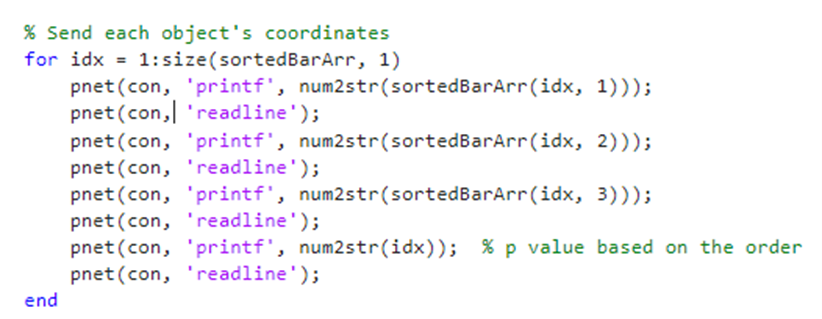
\includegraphics[width=4.5in ]{pics/MVOE.png}
    \label{PIC}
\end{figure}

\subsection{Data Transmission:}
The data sent between \texttt{MATLAB} and the \texttt{RAPID} program consists of the bar coordinates (\texttt{X}, \texttt{Y}), rotation (\texttt{R}), and a property value (\texttt{p}). The communication follows these steps:
\begin{enumerate}
    \item \texttt{MATLAB} establishes a TCP/IP socket connection to the robot controller.
    \item \texttt{MATLAB} sends the \texttt{X} coordinate of the first bar.
    \item \texttt{RAPID} receives the \texttt{X} coordinate and sends an acknowledgment back to \texttt{MATLAB}.
    \item \texttt{MATLAB} sends the \texttt{Y} coordinate of the first bar.
    \item It is repeated for the \texttt{R} and \texttt{p} values of the first bar and continues for the subsequent bars.
    \item After receiving all coordinates, the \texttt{RAPID} program processes the data for pick and place operations.
\end{enumerate}


%\newpage
\section{Forward and Inverse Kinematics Analysis: ABB IRB 120}
The task of solving the inverse kinematics for the ABB IRB 120 robot arm is a critical challenge in robotic system design and trajectory planning. Inverse kinematics involves calculating the joint angular positions required to achieve a desired position and orientation of the robot's end-effector. This process is a reverse computation of forward kinematics, where the known joint angles determine the position and orientation of the end-effector. The aim of solving an inverse kinematics solution is to enable the robot arm to interact with its environment in a controlled and predictable manner. This is essential for tasks requiring precision and repeatability. It is also important to note that the solution to the inverse kinematics problem is not unique, meaning that multiple joint configurations can result in the same end-effector position and orientation. Due to its mechanical constraints, the IRB 120 can have up to four different configurations to achieve a targeted end-effector state.

\subsection{Objectives}
\begin{enumerate}
  \item To create a three-dimensional representation of the ABB IRB 120 robot using the Robotics Toolbox for MATLAB\textsuperscript{\textregistered} in the open-source MATLAB\textsuperscript{\textregistered} environment.

  \item To derive and solve the forward and inverse kinematics equations for the ABB IRB 120 robot.

  \item To simulate the robot motion using the Robotics Toolbox for MATLAB\textsuperscript{\textregistered} with the implemented inverse kinematics solutions.
\end{enumerate}

\subsection{Choice of Robot}
For this task, the ABB IRB 120 is used. This robot is known for its compact and agile design, which makes it suitable for a wide range of applications. The IRB 120 is an articulated robot with six degrees of freedom (DOF), allowing for complex movements and high flexibility in task execution.

\noindent The key specifications of the ABB IRB 120 robot are as follows:
\begin{itemize}
  \item \textbf{Degrees of Freedom (DOF):} 6
  \item \textbf{Payload Capacity:} 3 kg
  \item \textbf{Reach:} 580 mm
  \item \textbf{Repeatability:} ±0.01 mm
  \item \textbf{Weight:} 25 kg
  \item \textbf{Wrist Type:} Spherical wrist
\end{itemize}

\noindent The IRB 120's spherical wrist and six axes of movement provides the need for precision in its operation. Its lightweight design, combined with enough payload capacity relative to its size, makes it an ideal choice for educational institutions and learning purposes as well. The robot's dimensions, gotten from the datasheet are as shown below:

\begin{figure}[H]
  \centering
  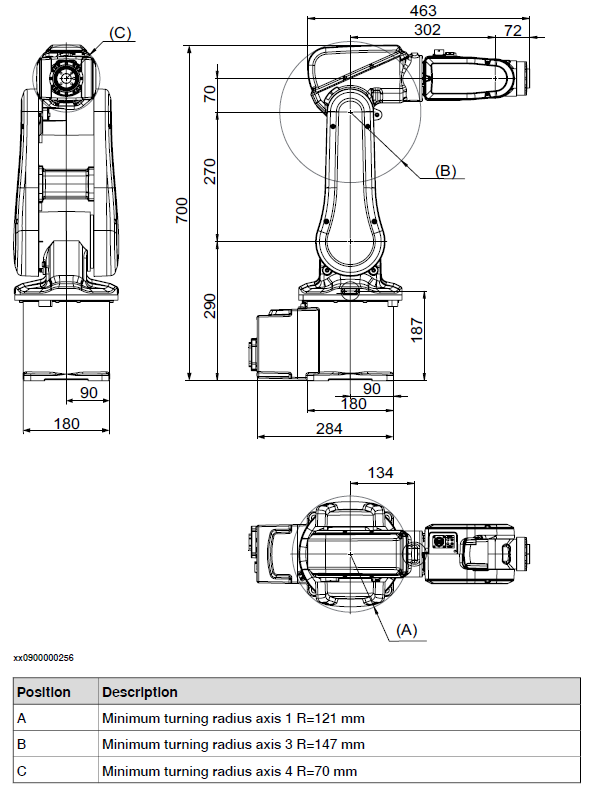
\includegraphics[width=4.8in ]{pics/dimensions_abb.png}
  \caption{ABB IRB 120 Robot Dimensions}\label{dimensions_abb}
\end{figure}


\subsection{Kinematic Representation}

Numerous methods exist for the kinematic representation of robot manipulators, and in this task, we will be using the formulation introduced by Denavit and Hartenberg. The D-H parameters are a set of four values that define the relative position and orientation between adjacent links in a robotic arm. For each joint/link of the robot, the following parameters are assigned:


\begin{itemize}
  \item \textbf{$a_i$:} The distance along the common normal from the z-axis of the previous joint to the z-axis of the current joint.
  \item \textbf{$\alpha_i$:} The angle about the common normal from the z-axis of the previous joint to the z-axis of the current joint. This describes the orientation of one link relative to the previous link.
  \item \textbf{$d_i$:} The offset distance along the previous z-ax s to the common normal, which can vary for prismatic joints.
  \item \textbf{$\theta_i$:} The angle about the previous z-axis from the previous x-axis to the current x-axis, which can vary for revolute joints.
\end{itemize}

\noindent The figure provided below illustrates the established coordinate systems for the Denavit-Hartenberg links as displayed on the manipulator.

\begin{figure}[H]
  \centering
  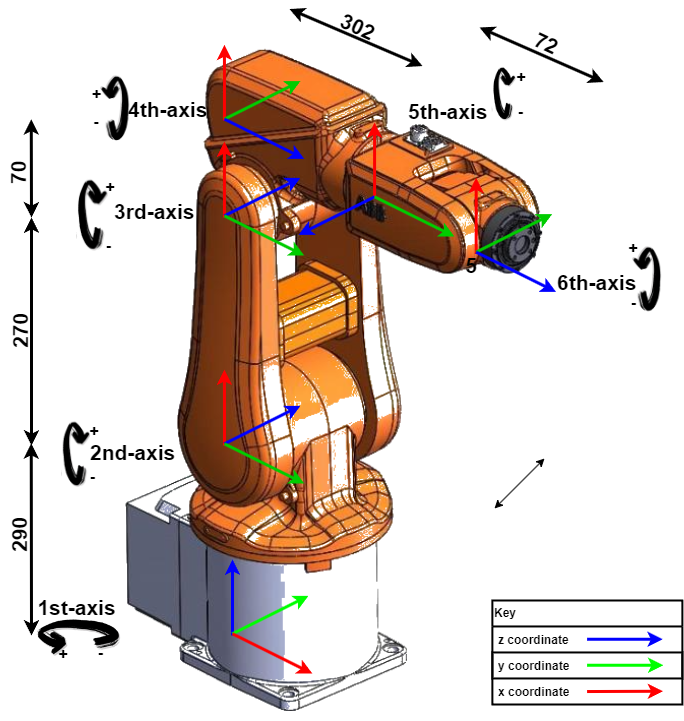
\includegraphics[width=3.6in ]{pics/coordinate frames abb120.drawio.png}
  \caption{ABB IRB 120 Robot with assigned coordinate frames}\label{assigned_coordinates}
\end{figure}


\noindent After defining the coordinate system, the robot’s configuration can be represented using the four D-H parameters explained previously: the joint angle ($\theta_i$), link length ($d_i$), offset distance ($a_i$), and twist angle ($\alpha_i$). Table 1 gives the D-H parameters associated with each link.



% Define the color for the header row
\definecolor{headercolor}{gray}{0}
\renewcommand{\arraystretch}{1.3}

\begin{table}[H]
  \centering\label{tab:dh_parameters}
  \resizebox{0.42\textwidth}{!}{
    \begin{tabular}{|c|c|c|c|}
      \hline
      \rowcolor{headercolor} \color{white}$\theta$ & \color{white}$d$ (mm) & \color{white}$a$ (mm) & \color{white}$\alpha$ (rad) \\
      \hline
      $\theta_1$                                   & 290                   & 0                     & $-\frac{\pi}{2}$            \\
      \hline
      $\theta_2 - \frac{\pi}{2}$                   & 0                     & 270                   & 0                           \\
      \hline
      $\theta_3$                                   & 0                     & 70                    & $-\frac{\pi}{2}$            \\
      \hline
      $\theta_4$                                   & 302                   & 0                     & $\frac{\pi}{2}$             \\
      \hline
      $\theta_5$                                   & 0                     & 0                     & $-\frac{\pi}{2}$            \\
      \hline
      $\theta_6 + {\pi}$                           & 72                    & 0                     & 0                           \\
      \hline
    \end{tabular}
  }
  \caption{DH Parameters of ABB IRB 120}
\end{table}

\noindent
\noindent For a serial-link manipulator with \( n \) joints, the position and orientation of the end-effector with respect to the base frame can be determined by the product of \( n \) homogeneous transformation matrices \( A_i \), each representing the transformation from frame \( i-1 \) to frame \( i \). The transformation matrix for joint \( i \) is given by:
\noindent
\[
  A_i = Rot(z, \theta_i) \cdot Trans(z, d_i) \cdot Trans(x, a_i) \cdot Rot(x, \alpha_i)
\]

where the rotation and translation matrices are defined as:
\noindent
\begin{align*}
  Rot(z, \theta_i) & = \begin{bmatrix}
                         \cos(\theta_i) & -\sin(\theta_i) & 0 & 0 \\
                         \sin(\theta_i) & \cos(\theta_i)  & 0 & 0 \\
                         0              & 0               & 1 & 0 \\
                         0              & 0               & 0 & 1
                       \end{bmatrix}, &
  Trans(z, d_i)    & = \begin{bmatrix}
                         1 & 0 & 0 & 0   \\
                         0 & 1 & 0 & 0   \\
                         0 & 0 & 1 & d_i \\
                         0 & 0 & 0 & 1
                       \end{bmatrix},                          
\end{align*}
\begin{align*}
  Trans(x, a_i)    & = \begin{bmatrix}
                         1 & 0 & 0 & a_i \\
                         0 & 1 & 0 & 0   \\
                         0 & 0 & 1 & 0   \\
                         0 & 0 & 0 & 1
                       \end{bmatrix},                          &
  Rot(x, \alpha_i) & = \begin{bmatrix}
                         1 & 0              & 0               & 0 \\
                         0 & \cos(\alpha_i) & -\sin(\alpha_i) & 0 \\
                         0 & \sin(\alpha_i) & \cos(\alpha_i)  & 0 \\
                         0 & 0              & 0               & 1
                       \end{bmatrix}.
\end{align*}

The final transformation matrix \( A_i \) is given by:
\[
  A_i = \begin{bmatrix}
    \cos(\theta_i) & -\sin(\theta_i)\cos(\alpha_i) & \sin(\theta_i)\sin(\alpha_i)  & a_i\cos(\theta_i) \\
    \sin(\theta_i) & \cos(\theta_i)\cos(\alpha_i)  & -\cos(\theta_i)\sin(\alpha_i) & a_i\sin(\theta_i) \\
    0              & \sin(\alpha_i)                & \cos(\alpha_i)                & d_i               \\
    0              & 0                             & 0                             & 1
  \end{bmatrix}
\]

\noindent The overall transformation matrix \( T \), which describes the pose of the end-effector, is the product of the individual transformation matrices:
\noindent
\[
  T = A_1 A_2 \cdots A_n
\]

\noindent This matrix \( T \) is a \( 4 \times 4 \) homogeneous transformation matrix that contains the position and orientation of the end-effector in its last column and the orientation of the end-effector in the first three columns.


\subsection{Computing Forward Kinematics}
To calculate the forward kinematics of the ABB IRB120 robot, we multiplied all the six A matrices to obtain the final transformation matrix. Alternatively, we used the \texttt{fkine} \cite{RoboticsToolbox} method provided by the Robotics Toolbox for MATLAB\textsuperscript{\textregistered} to confirm if our matrix multiplication was correct and it provided the same values. This method simplifies the process of computing the forward kinematics by taking the joint angles as input and returning the homogeneous transformation matrix representing the pose of the robot's end-effector. Given a set of joint angles, the \texttt{fkine} function computes the position and orientation of the end-effector. By comparing the computed end-effector position \((p_x, p_y, p_z)\) with the position obtained from the RobotStudio\textsuperscript{\textregistered} simulation software (TCP), we can verify the accuracy of our forward kinematics model. If the positions match, it confirms that our forward kinematics computation is correct. The MATLAB\textsuperscript{\textregistered} code for computing the forward kinematics is included in the appendix. After executing the MATLAB\textsuperscript{\textregistered} code, we obtain the position and orientation of the robot's end-effector. The results are then compared with the TCP values from the RobotStudio\textsuperscript{\textregistered} simulation to validate the forward kinematics model. The output from MATLAB\textsuperscript{\textregistered} is as shown below:

\begin{verbatim}
End-effector position: px = -163.9205700, py = -189.00, pz = 711.00
Full Transformation Matrix T:
     0.7704    0.1883   -0.6091    -163.9
    -0.5529    0.6731   -0.4912      -189
     0.3174    0.7152    0.6227       711
          0         0         0         1
\end{verbatim}


\noindent This output can be compared with the end-effector position obtained from the RobotStudio\textsuperscript{\textregistered} simulation, which is given as:

\begin{verbatim}
-162.38 -190.32 711.02
\end{verbatim}

\noindent It is depicted below:

\begin{figure}[H]
  \centering
  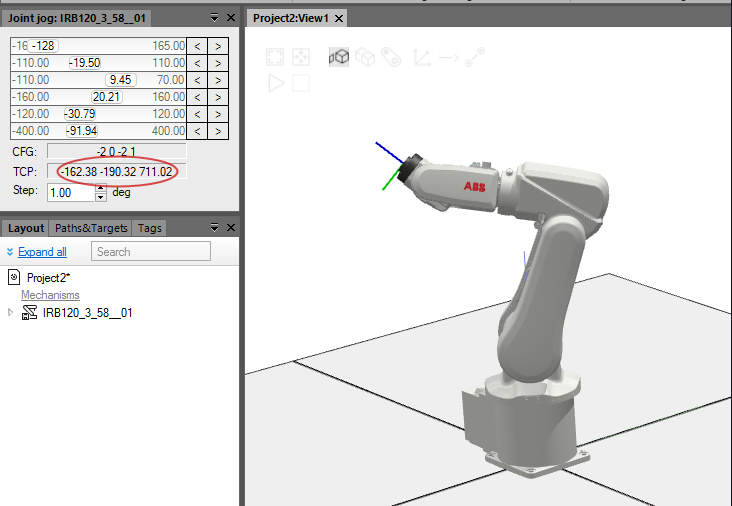
\includegraphics[width=5.2in ]{pics/rstudi.png}
  \caption{Joint Jog interface showing the end-effector position in RobotStudio\textsuperscript{\textregistered}.}\label{joint_jog}
\end{figure}



\noindent Given that the same joint angles are input into both the MATLAB\textsuperscript{\textregistered} function and the RobotStudio\textsuperscript{\textregistered} simulation, we can calculate the percentage error for the end-effector position coordinates to assess the accuracy of the forward kinematics model. The percentage error for each coordinate is calculated as follows:

\[
  \text{Percentage Error} = \left| \frac{\text{Actual Value} - \text{Simulated Value}}{\text{Simulated Value}} \right| \times 100
\]
\\
For the \( p_x \), \( p_y \), and \( p_z \) coordinates, the percentage errors are:

\[
  \text{Percentage Error}_{p_x} = \left| \frac{-163.92 - (-162.38)}{-162.38} \right| \times 100 \approx 0.95\%
\]
\[
  \text{Percentage Error}_{p_y} = \left| \frac{-189.00 - (-190.32)}{-190.32} \right| \times 100 \approx 0.69\%
\]
\[
  \text{Percentage Error}_{p_z} = \left| \frac{711.00 - 711.02}{711.02} \right| \times 100 \approx 0.0028\%
\]
\noindent
\noindent The slight differences observed between the MATLAB\textsuperscript{\textregistered} output and the RobotStudio\textsuperscript{\textregistered} simulation can be attributed to various factors, including numerical rounding errors in the computation, differences in the internal representation of joint angles, or slight variations in the robot model used in the simulation compared to the theoretical model used in the MATLAB\textsuperscript{\textregistered} computation.

\begin{table}[H]
  \centering\label{tab:percentage_error}
  \begin{tabular}{|c|c|c|}
    \hline
    \rowcolor{black} \color{white}Coordinate & \color{white}MATLAB Value & \color{white}Percentage Error \\
    \hline
    \( p_x \)                                & -163.92                   & 0.95\%                        \\
    \hline
    \( p_y \)                                & -189.00                   & 0.69\%                        \\
    \hline
    \( p_z \)                                & 711.00                    & 0.0028\%                      \\
    \hline
  \end{tabular}
  \caption{Percentage Error in End-Effector Position}
\end{table}


\newpage
\subsection{Inverse Kinematics}
Inverse kinematics for the ABB IRB 120 robot, which has six degrees of freedom (DOF) with all revolute joints and a spherical wrist, can be efficiently solved using the kinematic decoupling approach as described by Seth Hutchinson and Mark W. Spong in \textit{Robot Modeling and Control} \cite{Modeling}. This approach simplifies the complex inverse kinematics problem into two manageable sub-problems: inverse position kinematics and inverse orientation kinematics \cite{Modeling}.

\subsubsection{Kinematic Decoupling}
The kinematic decoupling method is particularly useful for manipulators with six joints where the last three joint axes intersect at a common point, forming a spherical wrist \cite{Modeling}. Other types of robot manipulators can also have a spherical wrist in different setups like RPP + Spherical Wrist (R for Revolute, P for Planar), RRP Spherical Manipulator and so on. This allows the inverse kinematics problem to be divided into finding the position of the wrist center and determining the orientation of the wrist.

\noindent For a six-DOF manipulator with a spherical wrist, the inverse kinematics can be broken into two steps:

\begin{enumerate}
  \item  \textbf{Position problem:} Finding the position of the wrist center (\(\theta_1\)\(\theta_2\)\(\theta_3\)).
  \item  \textbf{Orientation problem}: Determining the orientation of the wrist (\(\theta_4\)\(\theta_5\)\(\theta_6\)).
\end{enumerate}


\begin  {figure}[H]
\centering
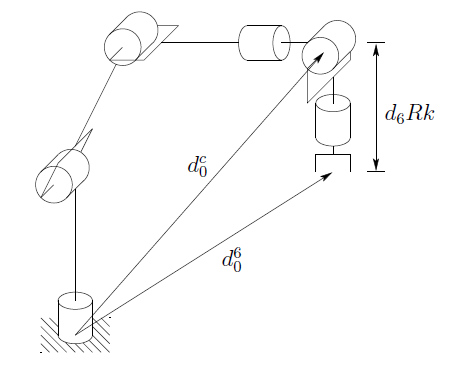
\includegraphics[width=3.5in]{pics/inverse_hutchinson.png}
\caption {Illustration of Kinematic Decoupling \cite{Modeling}}
\label{fig:kinematic_decoupling}
\end{figure}

\subsubsection{Determining Origin of Spherical Wrist}
So we will start our workings from the wrist centre, but the problem is we do not know where the wrist centre is, in terms of its coordinates / location. To find the location of the origin of the wrist, we will come back from the end effector (Joint 6) and offset by \(z_6\) to get to wrist position origin.
\noindent This offset is 72 mm along the \(Z_6\) direction, and we use the last column of the rotation matrix to represent \(Z_6\) in the base frame. By subtracting this offset, we obtain the wrist center position (\(\mathbf{o}_c^0\)):

\[
  \mathbf{o}_c^0 = \mathbf{o}_6^0 - d_6 \mathbf{z}_6^0 = \mathbf{o}_6^0 -72{R}_6^0
\]

\noindent where \(\mathbf{o}_c^0\) is the end-effector position, \(d_6\) is the offset distance 72 mm, \(\mathbf{o}_6^0\) is the \((p_x, p_y, p_z)\) of the final transformation matrix, and \(\mathbf{R}_6^0\) is the unit vector along \(Z_6\). To understand this better, this can be represented in component form as follows:

\[
  \begin{pmatrix}
    x_c \\
    y_c \\
    z_c
  \end{pmatrix} =
  \begin{pmatrix}
    o_x \\
    o_y \\
    o_z
  \end{pmatrix} -
  d_6
  \begin{pmatrix}
    r_{13} \\
    r_{23} \\
    r_{33}
  \end{pmatrix}
\]

\noindent where \(p_x\), \(p_y\), and \(p_z\) are the components of the desired end-effector position, and \(r_{13}\), \(r_{23}\), and \(r_{33}\) are the elements of the third column of the rotation matrix \(\mathbf{R}\). This can be seen in the rough sketch below.

\begin{figure}[H]
  \centering
  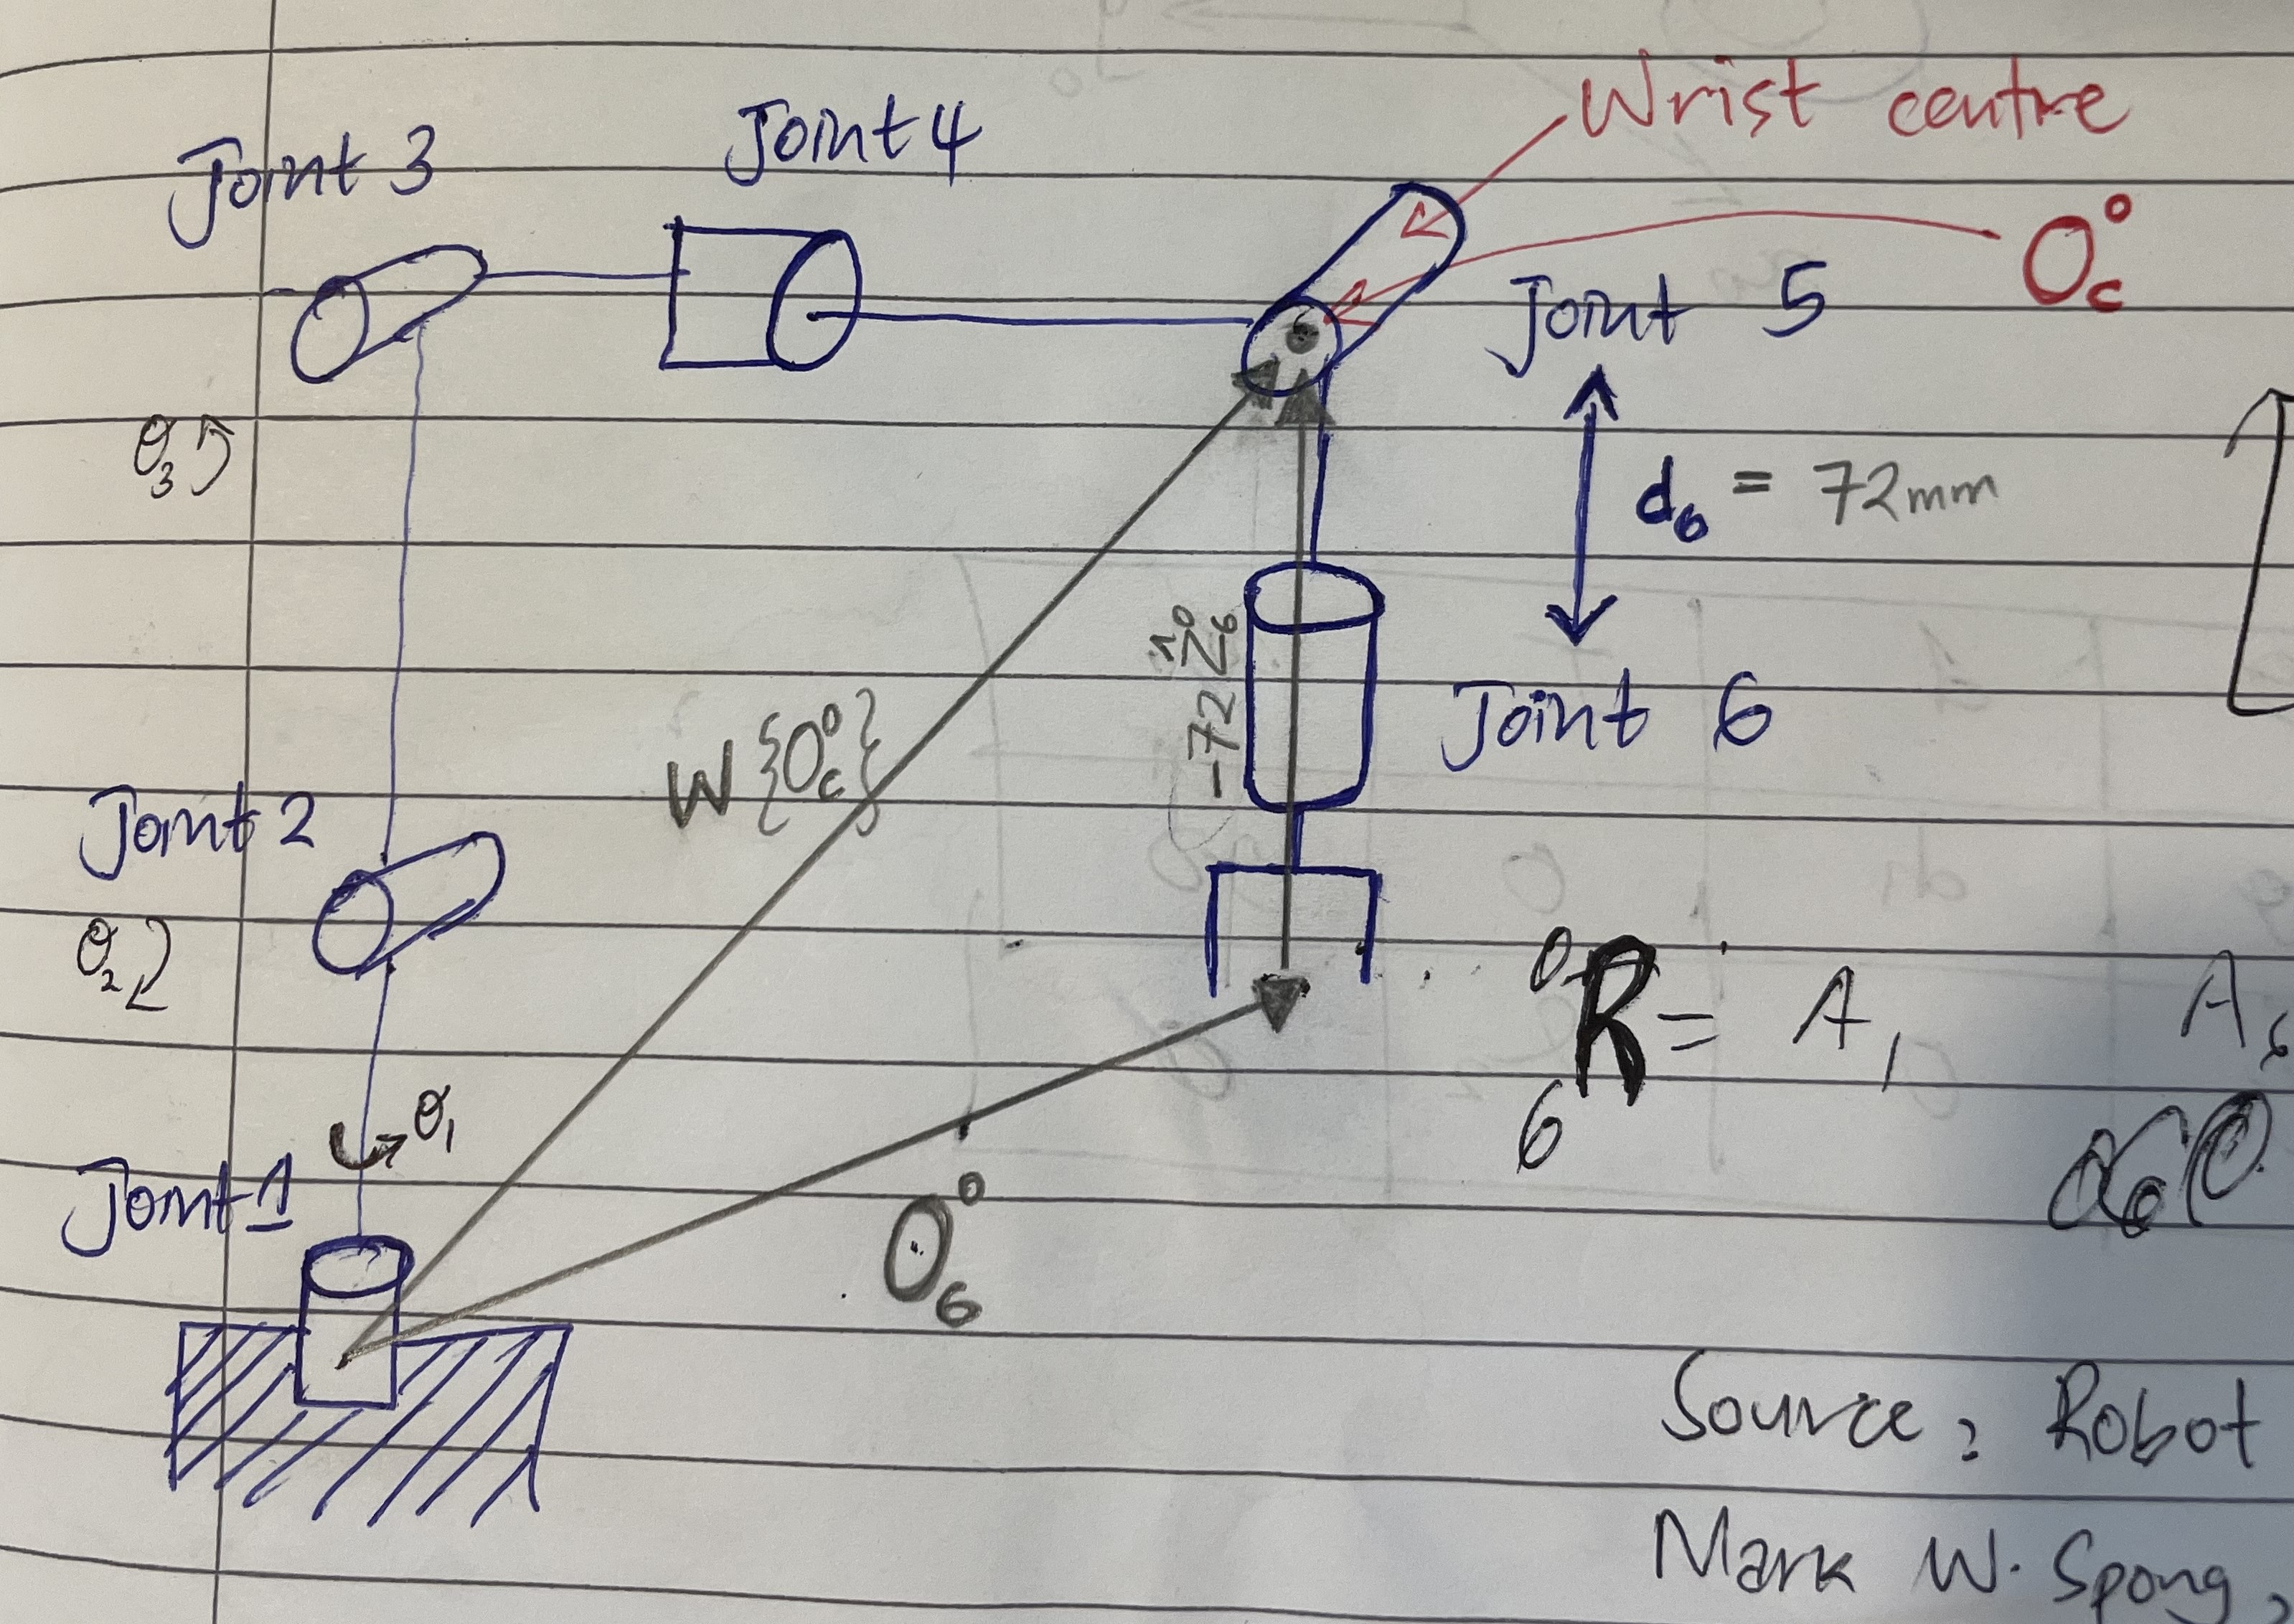
\includegraphics[width=4.0in ]{pics/decoup_sketch.JPG}
  \caption{Sketch of spherical wrist .}
  \label{sphericalw}
\end{figure}


\noindent Next, we define the transformation matrices (\(A_1\) to \(A_6\)) for each joint using the DH parameter. These will be the inputs for the orientation of the object when we finally solve the inverse kinematics and have to input the position and orientation of the object to find the joint angles. In the MATLAB\textsuperscript{\textregistered} code, this is implemented here:

\begin{lstlisting}[frame=single,style=Matlab-Pyglike]
% Prompt for end effector position and orientation
O60 = input('Enter the end effector position as a 3-element vector [x; y; z]: ');
R60 = input('Enter the end effector orientation as a 3x3 rotation matrix: ');
Oc0 = O60 - 72 * R60(:,3);   % wrist position
\end{lstlisting}




\subsubsection{Determining Position of Wrist \texorpdfstring{$\left(p_x, p_y, p_z\right)$}{px, py, pz} of \texorpdfstring{$\left(\mathbf{T}_4^0\right)$}{T40}}

The location of the wrist depends only on \(\theta_1\), \(\theta_2\), and \(\theta_3\). \(\theta_4\) only accounts for the distance 302 mm because it rotates about axis \(Z_3\), which doesn’t change the position of the point.. So this means that we will only consider the transformation matrix from the DH parameters until the fourth A matrix.

\[
  T_4^0 = A_1 \cdot A_2 \cdot A_3 \cdot A_4
\]

\noindent In the MATLAB code, the function  this is implemented here:

\begin{lstlisting}[frame=single,style=Matlab-editor]
T40 = A1*A2*A3*A4;

disp('Wrist position (considered upto link 4)');
wp = simplify(T40(1:3,4));  % last column, px py pz
disp(wp)
\end{lstlisting}


\subsubsection{Determining \texorpdfstring{$\theta_1$, $\theta_2$, and $\theta_3$}{theta1, theta2, and theta3}}

\noindent After having determined the wrist center position from MATLAB, \(T_4^0\), it is given by:

\[
  \left(\begin{array}{c}
      2\,\cos \left(\theta_1 \right)\,{\left(151\,\cos \left(\theta_2 +\theta_3 \right)+35\,\sin \left(\theta_2 +\theta_3 \right)+135\,\sin \left(\theta_2 \right)\right)} \\
      2\,\sin \left(\theta_1 \right)\,{\left(151\,\cos \left(\theta_2 +\theta_3 \right)+35\,\sin \left(\theta_2 +\theta_3 \right)+135\,\sin \left(\theta_2 \right)\right)} \\
      270\,\cos \left(\theta_2 \right)+2\,\sqrt{24026}\,\cos \left(\theta_2 +\theta_3 +\mathrm{atan}\left(\frac{151}{35}\right)\right)+290
    \end{array}\right)
\]

\noindent Since the position depends only on \(\theta_1\), \(\theta_2\), and \(\theta_3\), we can solve for these angles.

\noindent For \(\theta_1\):

The wrist center's \(x\) and \(y\) coordinates can be written as:
\[
  p_x = 2\,\cos(\theta_1)\,k
\]
\[
  p_y = 2\,\sin(\theta_1)\,k
\]

where
\[
  k = 151\,\cos(\theta_2 + \theta_3) + 35\,\sin(\theta_2 + \theta_3) + 135\,\sin(\theta_2)
\]

By eliminating \(k\), we have:
\[
  \tan(\theta_1) = \frac{p_y}{p_x}
\]

\begin{center}
  \shadowbox{
    \(\theta_1 = \tan^{-1}\left(\frac{p_y}{p_x}\right)
    \)
  }
\end{center}


\noindent For \(\theta_2\) and \(\theta_3\), using trigonometric identities:
\[
  \sin(\theta_1)\cos(\theta_2) + C_1\sin(\theta_2) = S_{12}
\]
\[
  \cos(\theta_1)\cos(\theta_2) - S_1\sin(\theta_2) = C_{12}
\]

where \(C_1 = \cos(\theta_1)\), \(S_1 = \sin(\theta_1)\), \(C_{12} = \cos(\theta_2 + \theta_3)\), and \(S_{12} = \sin(\theta_2 + \theta_3)\).

\noindent Simplifying the \(z\)-coordinate of the wrist position:
\[
  p_z = 270\,\cos(\theta_2) + 2\,\sqrt{24026}\,\cos\left(\theta_2 + \theta_3 + \mathrm{atan}\left(\frac{151}{35}\right)\right) + 290
\]




Using the trigonometric identity:
\[
  \cos(a + b) = \cos(a)\cos(b) - \sin(a)\sin(b)
\]

we can solve for \(\theta_2\) and \(\theta_3\) by substituting and simplifying the equations.

\noindent Since \(\tan (\beta) = \frac{151}{35}\), we look for \(\cos (\beta)\) and \(\sin (\beta)\)

Using Pythagoras' theorem,
\[
  a^2 + b^2 = c^2
\]
\[
  \tan^{-1}(\theta) = \frac{a}{b} \implies \cos (\theta) = \frac{a}{c}
\]
\[
  c^2 = \sqrt{a^2 + b^2}
\]

In tangent, \(c = \frac{a}{\tan (\theta)}\)
\[
  a^2 = (c \cdot \tan (\theta))^2
\]
\[
  c^2 = a^2 + (a \cdot \tan (\theta))^2
\]
\[
  c = a \sqrt{1 + \tan^2 (\theta)}
\]
\[
  a = \frac{c}{\sqrt{1 + \tan^2 (\theta)}}
\]

So \(\cos (\beta)\) is:
\[
  \cos (\beta) = \frac{1}{\sqrt{1 + \tan^2 (\beta)}} = \frac{1}{\sqrt{1 + \left( \frac{151}{35} \right)^2}} = \frac{1}{\sqrt{1 + \frac{22801}{1225}}} = \frac{1}{\sqrt{\frac{24026}{1225}}} = \frac{\sqrt{1225}}{\sqrt{24026}} = \frac{35}{\sqrt{24026}}
\]





\[
  \sin (\beta) = \cos (\beta) \cdot \tan (\beta) = \frac{35}{\sqrt{24026}} \cdot \frac{151}{35} = \frac{151}{\sqrt{24026}}
\]

So,
\[
  \cos (\theta_2 + \theta_3 + \beta) = \cos (\theta_2 + \theta_3) \frac{35}{\sqrt{24026}} - \sin (\theta_2 + \theta_3) \frac{151}{\sqrt{24026}}
\]

\[
  270 \cos (\theta_2) + 2 \sqrt{24026} \cdot \left[ \cos (\theta_2 + \theta_3) \frac{35}{\sqrt{24026}} - \sin (\theta_2 + \theta_3) \frac{151}{\sqrt{24026}} \right] + 290
\]

\[
  = 270 \cos (\theta_2) + 70 \cos (\theta_2 + \theta_3) - 302 \sin (\theta_2 + \theta_3) + 290
\]

\noindent Wrist position with Trigonometry simplification:
\[
  \begin{aligned}
    C_1 (302 \cos (\theta_3) + 70 \sin (\theta_2 + \theta_3) + 270 \sin (\theta_2))            & = X_c       \\
    S_1 (302 \cos (\theta_3) + 70 \sin (\theta_2 + \theta_3) + 270 \sin (\theta_2))            & = Y_c       \\
    270 \cos (\theta_2) + 70 \cos (\theta_2 + \theta_3) - 302 \sin (\theta_2 + \theta_3) + 290 & = Z_c - 290
  \end{aligned}
\]



\noindent Square the 3 equations to eliminate \( \theta_1 \), i.e., \( C_1 \) and \( S_1 \)

\begin{align*}
   & X_c^2 + Y_c^2 + (Z_c - 290)^2 = (302 \cos (\theta_3) + 70 \sin (\theta_2 + \theta_3) + 270 \sin (\theta_2))^2 \\
   & + (270 \cos (\theta_2) + 70 \cos (\theta_2 + \theta_3) - 302 \sin (\theta_2 + \theta_3))^2
\end{align*}


Assuming it's a quadratic equation:
\[
  \frac{-b \pm \sqrt{b^2 - 4ac}}{2a}
\]

Substitute \(S_3\) into the equation:
\[
  C = A \cdot C_3 + B \cdot \sqrt{1 - C_3^2}
\]

\[
  C^2 = (A \cdot C_3)^2 + (B \cdot \sqrt{1 - C_3^2})^2
\]

\[
  (A^2 + B^2) \cdot C_3^2 - 2AC \cdot C_3 + (C^2 - B^2) = 0
\]

\[
  \theta_3 = \cos^{-1} \left( \text{roots} \left( [A^2 + B^2, -2AC, C^2 - B^2] \right) \right)
\]

\noindent To solve for \(\theta_3\), we can use either the \(\cos^{-1}\) function or the \(\tan^{-1}\) function. The possible solutions for \(\theta_3\) are given by:

\begin{center}
  \shadowbox{
    \(\theta_3 = \cos^{-1} \left( \text{roots} \left( [A^2 + B^2, -2AC, C^2 - B^2] \right) \right)\)
  }
\end{center}


\noindent or using the \(\tan^{-1}\) function:

\begin{center}
  \shadowbox{
    \(\theta_3 = \tan^{-1} \left( \sqrt{1 - D(1)^2}, D(1) \right)\)
  }
\end{center}



\noindent The MATLAB\textsuperscript{\textregistered} code for finding \(\theta_3\) is as follows:
\begin{lstlisting}[frame=single,style=Matlab-editor]
% three equations from wrist position
A = 2 * (270^2);
B = 2 * 70 * 302 * 270;
% B=2*70*270;
%B=2*70*302;  % correct one
C = xc^2 + yc^2 + (zc - 290)^2 - 302^2 - 70^2 -270^2;
% D=acos(roots([A^2+B^2,-2*A*C,C^2-B^2]));
D = roots([A^2 + B^2, -2 * A * C, C^2 - B^2]);

% theta3 = D(1);
theta3 = atan2(sqrt(1 - D(1)^2), D(1));
\end{lstlisting}

\subsubsection{Calculating \texorpdfstring{$\theta_2$}{theta2}}

Once \(\theta_3\) is known, we factor out the coefficients of \(\theta_2\) from equation (3):
\[
  270C_2 + 70C_{23} - 302S_{23} = Z_c - 290 \\
\]
\noindent
\[
  C_2 \left( 270 + 70 C_3 - 302 S_3 \right) + S_2 \left( -70 S_3 + 302 C_3 \right) = Z_c - 290
\]


\noindent We can solve for \(\theta_2\) by forming a quadratic equation:
\[
  C_2 \left( 270 + 70 C_3 - 302 S_3 \right) + S_2 \left( -70 S_3 + 302 C_3 \right) = Z_c - 290
\]

The solution for \(\theta_2\) in terms of the MATLAB code is obtained as follows:

\begin{center}
  \shadowbox{
    \(\theta_2 = \mathrm{atan2}\left(-\sqrt{1 - D_2^2}, D_2\right)\)
  }
\end{center}
where \( D_2 \) is obtained from solving the quadratic equation:
\[
  AA^2 + BB^2, -2AA \cdot CC, CC^2 - BB^2
\]
with:
\[
  AA = 270 + 70 \cos(\theta_3) - 302 \sin(\theta_3)
\]
\[
  BB = -70 \sin(\theta_3) - 302 \cos(\theta_3)
\]
\[
  CC = Z_c - 290
\]

The value of \(\theta_2\) is then converted to degrees:
\[
  \theta_2^{\text{deg}} = \text{rad2deg}(\theta_2)
\]


\noindent The MATLAB\textsuperscript{\textregistered} code for solving \(\theta_2\) is as follows:
\begin{lstlisting}[frame=single,style=Matlab-editor]
AA = 270 + 70 * cos(theta3) - 302 * sin(theta3);
BB = -70 * sin(theta3) - 302 * cos(theta3);
CC = zc - 290;

% Solve the quadratic equation
DD = real(roots([AA^2 + BB^2, -2*AA*CC, CC^2 - BB^2]));
theta2 = real(atan2(-sqrt(1 - DD(2)^2), DD(2)));
theta2_deg = rad2deg(theta2);
fprintf('theta2 = %.3f radians, %.3f degrees\n', theta2, theta2_deg);
\end{lstlisting}





\begin{table}[H]
  \centering
  \begin{tabular}{|c|c|c|c|}
    \hline
    \(\theta\)                   & \(d\) (mm) & \(a\) (mm) & \(\alpha\) (rad)   \\
    \hline
    \(\theta_1\)                 & 290        & 0          & \(-\frac{\pi}{2}\) \\
    \hline
    \(\theta_2 - \frac{\pi}{2}\) & 0          & 270        & 0                  \\
    \hline
    \(\theta_3\)                 & 0          & 70         & \(-\frac{\pi}{2}\) \\
    \hline
    \(\theta_4\)                 & 302        & 0          & \(\frac{\pi}{2}\)  \\
    \hline
    \(\theta_5\)                 & 0          & 0          & \(-\frac{\pi}{2}\) \\
    \hline
    \(\theta_6 + \pi\)           & 72         & 0          & 0                  \\
    \hline
  \end{tabular}
  \caption{DH Parameters of ABB IRB 120}
\end{table}

\noindent We then multiply these matrices to get the forward kinematics transformation from the base frame to the end-effector (\(T_6^0\)). We also compute the transformation matrices up to the wrist (\(T_4^0\)), which we use to find the wrist position in terms of the first three joint angles.



\[
  T_6^0 = A_1 A_2 A_3 A_4 A_5 A_6
\]

\noindent By computing the transformation matrices up to the wrist center (\(T_4^0\)), we find the position of the wrist center in terms of \(\theta_1\), \(\theta_2\), and \(\theta_3\).


\subsubsection{Determining \texorpdfstring{$\theta_4$, $\theta_5$, and $\theta_6$}{theta4, theta5, and theta6}}

From the given rotation matrix:
\[
  R_6^0 = R_3^0 R_6^3
\]

\noindent where \(\mathbf{R}_0^3\) is the orientation matrix of the first three joints, and \(\mathbf{R}_3^6\) represents the orientation from the wrist frame to the end-effector frame \cite{Modeling}.
\[
  R_6^3 = (R_3^0)^T R_6^0
\]

Given \(R_6^3\):
\[
  \left( \begin{array}{ccc}
      \sin(\theta_4) \sin(\theta_6) - \cos(\theta_4) \cos(\theta_5) \cos(\theta_6)  & \cos(\theta_6) \sin(\theta_4) + \cos(\theta_4) \cos(\theta_5) \sin(\theta_6) & -\cos(\theta_4) \sin(\theta_5) \\
      -\cos(\theta_4) \sin(\theta_6) - \cos(\theta_5) \cos(\theta_6) \sin(\theta_4) & \cos(\theta_5) \sin(\theta_4) \sin(\theta_6) - \cos(\theta_4) \cos(\theta_6) & -\sin(\theta_4) \sin(\theta_5) \\
      -\cos(\theta_6) \sin(\theta_5)                                                & \sin(\theta_5) \sin(\theta_6)                                                & \cos(\theta_5)
    \end{array} \right)
\]

To determine \(q_4, q_5, q_6\):
\[
  R_6^3 = R_3^0 \left( R_6^0 \right)^T
\]

From the \(R_6^3\) matrix:

\begin{center}
  \shadowbox{
    \(\theta_5 = \arctan2 \left( \sqrt{R_{6,1}^3 + R_{6,2}^3}, R_{6,3}^3 \right)
    \)
  }
\end{center}

\begin{center}
  \shadowbox{
    \(\theta_6 = \arctan2 (R_{6,2}, -R_{6,1}))
    \)

  }
\end{center}

\begin{center}
  \shadowbox{
    \(\theta_4 = \arctan2 (-R_{6,2,3}, -R_{6,1,3})
    )
    \)
  }
\end{center}



\section{Development of 3D model and animation}
In this mini-task, we had to import the 3D model of the ABB IRB 120 robot into MATLAB\textsuperscript{\textregistered} and then visualize it with Robotics Toolbox for MATLAB\textsuperscript{\textregistered} developed by Peter Corke. From MATLAB's own documentation as shown below, MATLAB\textsuperscript{\textregistered}  reads geometry models as stl files.

\begin{figure}[H]
  \centering
  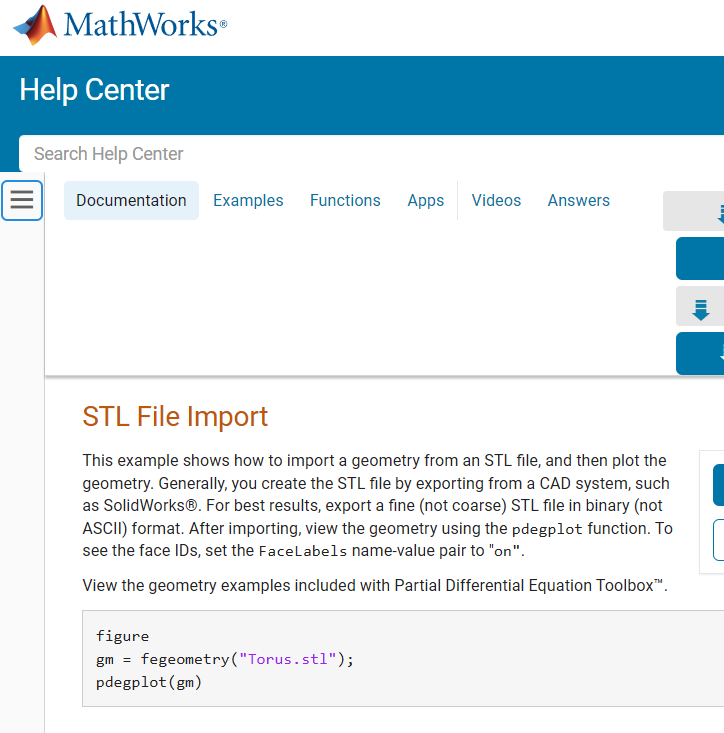
\includegraphics[width=2.0in ]{pics/stl.png}
  \caption{stl file import into MATLAB\textsuperscript{\textregistered}.}
  \label{stl}
\end{figure}



So we would have to obtain the robot's CAD models from the manufacturer's website, then edit them on a 3D CAD Software into individual parts. This is because MATLAB\textsuperscript{\textregistered} reads the .stl files for each link separately. The 3D model of the ABB 120 was found online but it was an assembly which was in .step format. I converted the individual parts into stl format and was using the SolidWorks' Move and Rotate feature to orient the link's origin so as it was consistent with the Denavit Hartenberg model (stick figure) we constructed earlier on MATLAB. I also had to scale down the modles by 1000 since the Robotics Toolbox uses metres as opposed to millimetres on SolidWorks. It is also important to note that upon reading on the book \textit{Robotics Toolbox for MATLAB} by Peter Corke, he specified the package ARTE by Arturo Gil \cite{ARTEARob24:online} which had already included the 3D models of some robots in the Robotics Toolbox (version 10.4), including the ABB IRB 120. The task would be as simple as downloading the stl files from ARTE's library \cite{ARTEARob24:online} and calling the function \texttt{Serialplot3D()}, while specifying the parameters.


\begin{figure}[H]
  \centering
  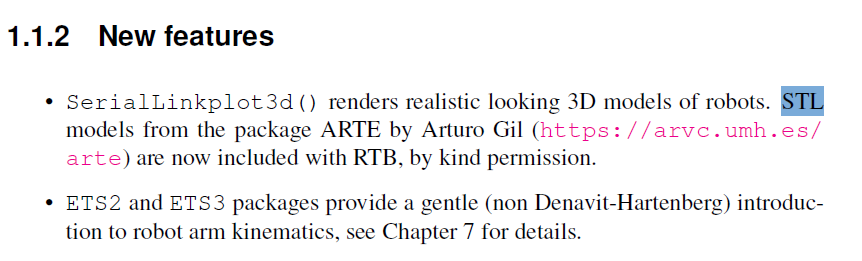
\includegraphics[width=3.0in ]{pics/Screenshot_7.png}
  \caption{ARTE package by Arturo Gil \cite{RoboticsToolbox}}
  \label{arte}
\end{figure}


The 3D model simulation can be seen on the below image:


\begin{figure}[H]
  \centering
  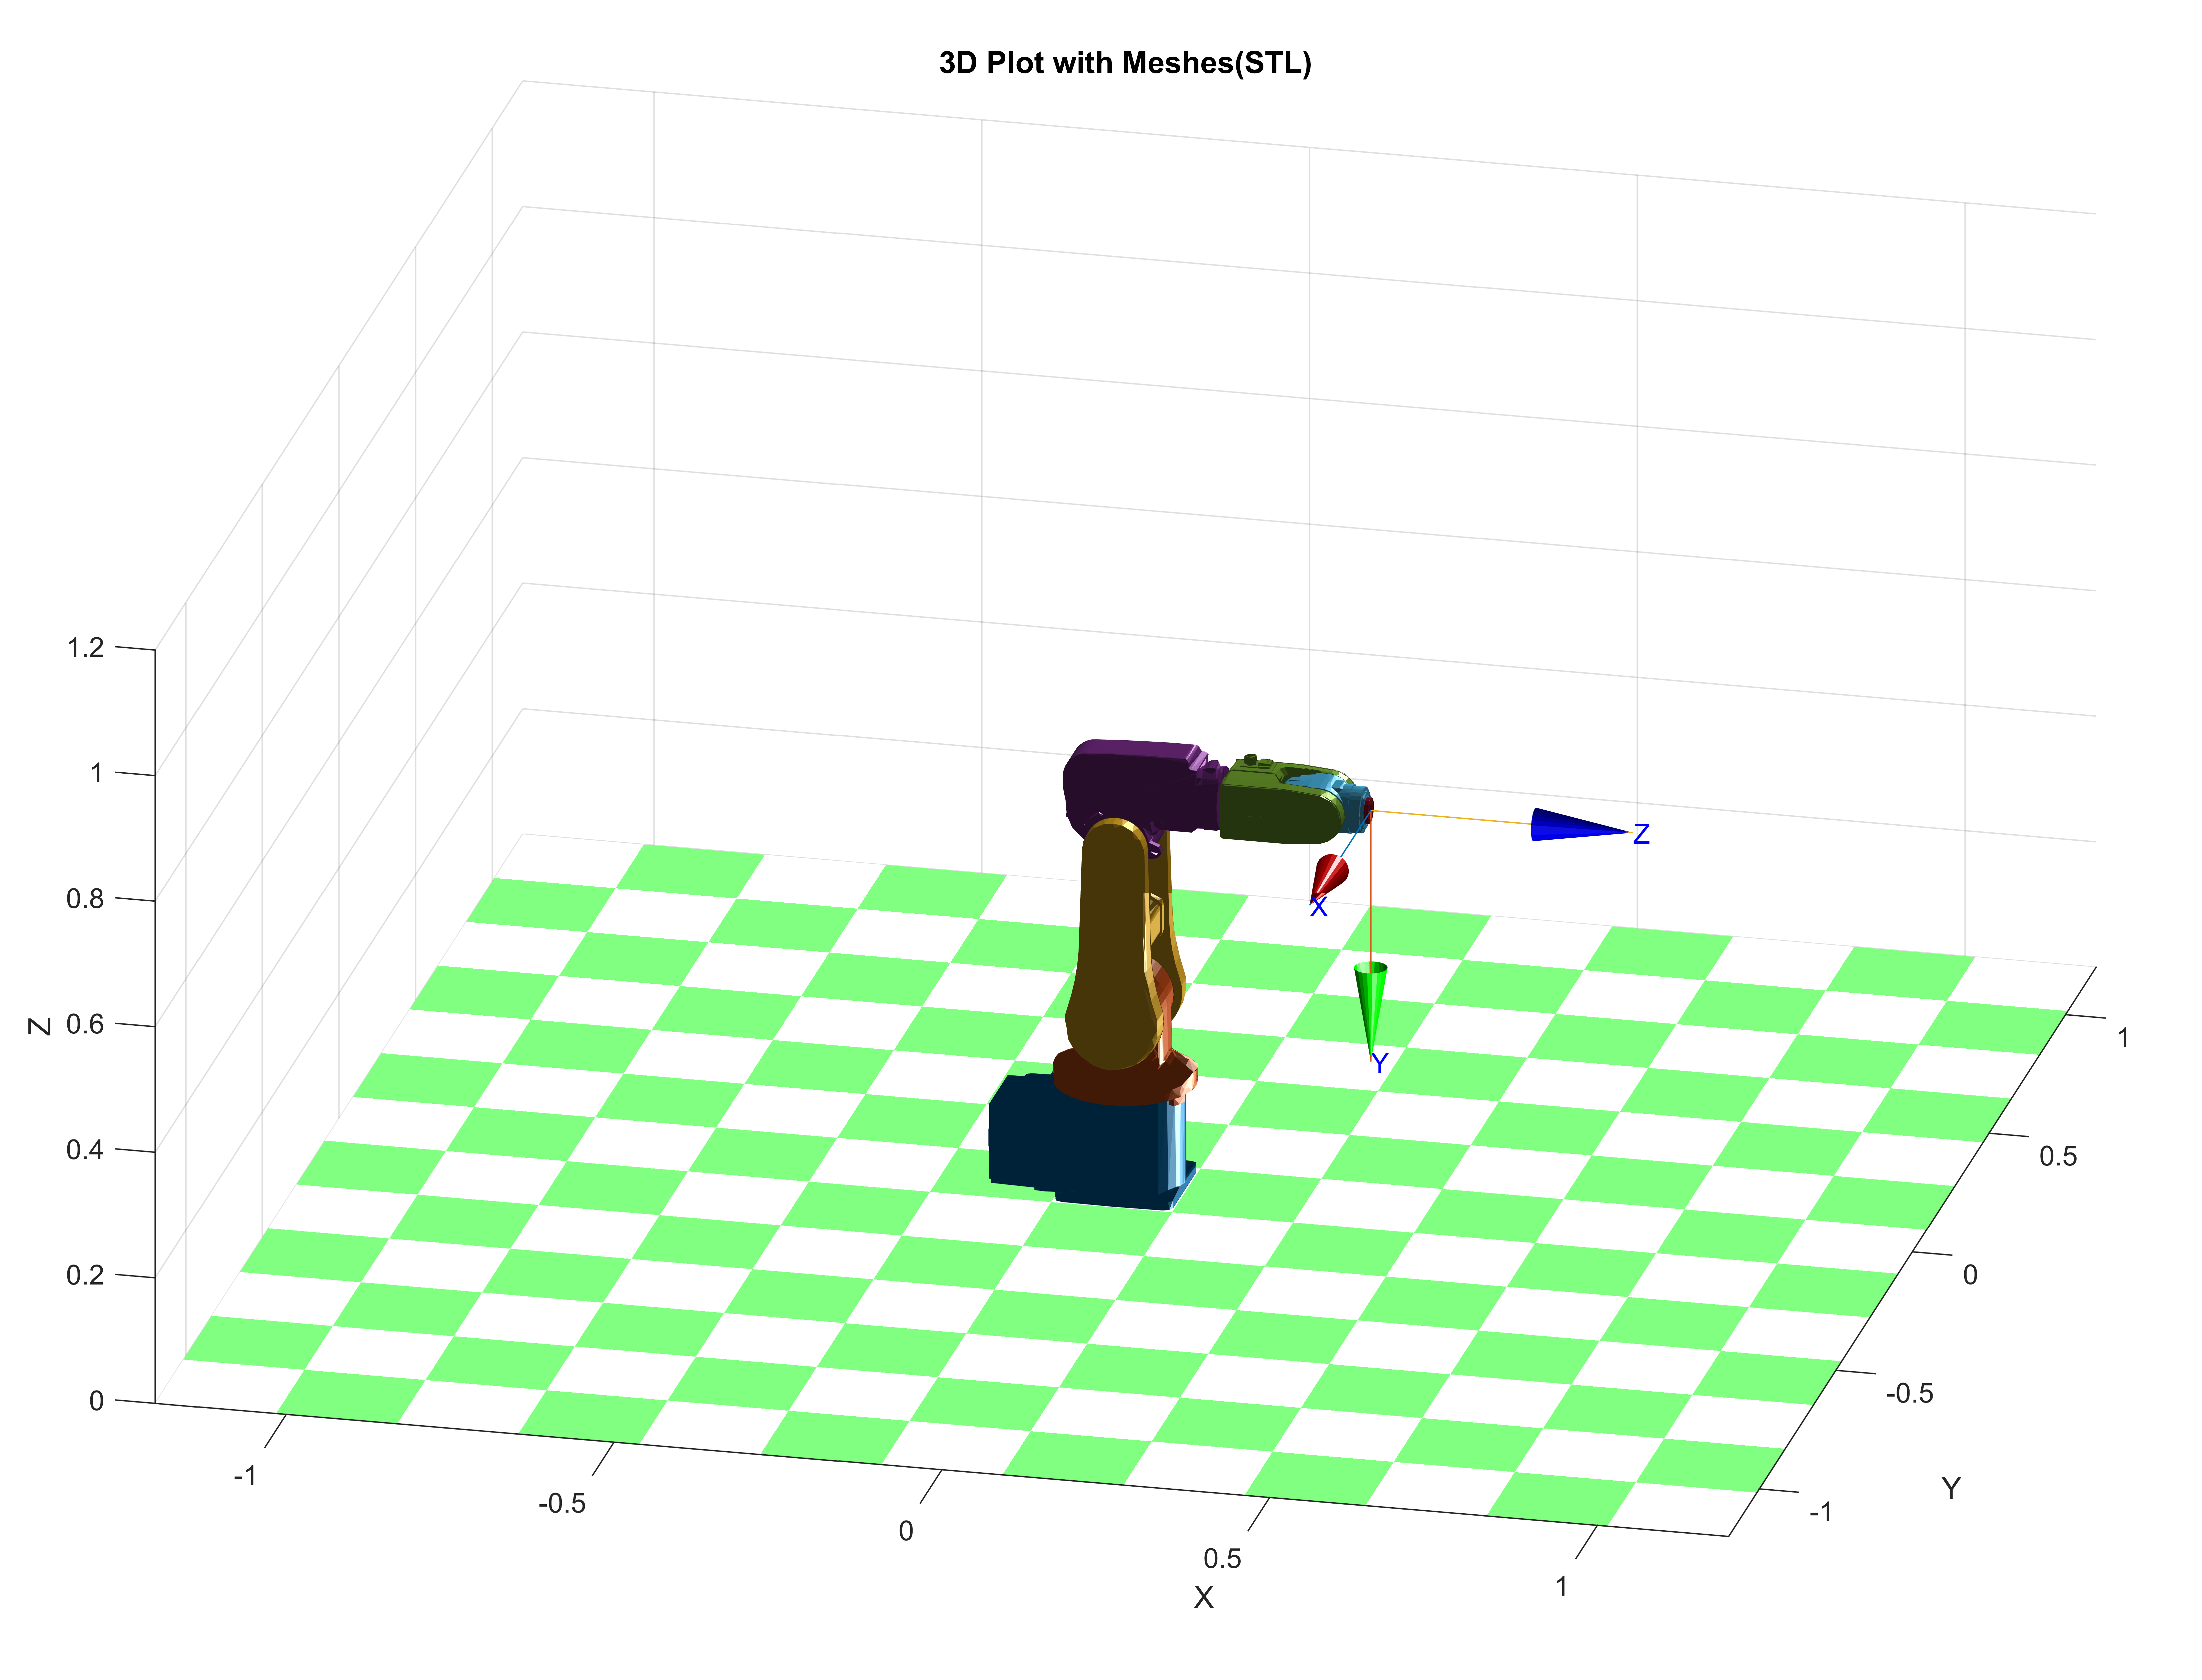
\includegraphics[width=3.6in ]{pics/3d stl.png}
  \caption{3D CAD Model Visualization on RTB}
  \label{3d}
\end{figure}



\subsection{Challenges encountered during 3D model animation}
After successfully importing the 3D model of the robot into MATLAB, we tried to
move the same way as the physical robot in the pick and place task. The image
coordinates were to be obtained from the Image Recognition code and then input
into the inverse kinematics solution. These inputs are three coordinates which is
the image x, y and its orientation. 

\noindent Unfortunately, this posed a challenge as our inverse kinematics solution failed to address this 
matter. To generate the appropriate joint angles, the inverse kinematics solution
required the image / object's x, y and z coordinates in 3d vector matrix as well
as its orientation (px, py and pz). The inverse kinematics solution totally failed
to address this issue and thus we could not animate the robot as based on the 
image coordinates. A suggestion was put that the image coordinates to be converted
to 3d vector format and since the z coordinate is already known, then this would 
be input to the inverse kinematic solution. Further research and understanding needs to be done in 
this area and appropriate solution needs to be done especially when calculating 
inverse of a six degrees of freedom robot using the analytical way. 





\section{Conclusion}
This project successfully demonstrates a robust method for integrating \texttt{MATLAB\textsuperscript{\textregistered}} and \texttt{RAPID} for pick and place operations using socket communication. The \texttt{RAPID} program efficiently handles the data received from \texttt{MATLAB\textsuperscript{\textregistered}}, sorts the objects based on a property value, and performs the pick and place operations to stack it at the \texttt{stackPoint} to form a pyramid structure. The
integration between \texttt{MATLAB\textsuperscript{\textregistered}} and the \texttt{ABB} robot controller through socket communication enables efficient and precise control of the robot arm for pick and place tasks based on real-time data from image processing. This setup can be adapted and extended for various industrial applications involving robotic automation. 
By implementing the kinematic decoupling approach, the inverse kinematics problem for the ABB IRB 120 robot can be solved, making it able to control of the robot's end-effector position and orientation.





\section*{Appendix}
\large\href{https://studentsswinburneedu-my.sharepoint.com/:f:/g/personal/101229220_students_swinburne_edu_my/EtwPYa2U7ctPskWgIqP-EhEBreegVWK0ACHmneuZSLz_TQ?e=V1dBor}{Link to Code files}



\clearpage
\phantomsection  % Helps with proper hyperref linking
% References 
\bibliographystyle{ieeetr}
\bibliography{references}




\end{document}


